\documentclass[12pt, a4paper, oneside]{report}

% ==========================================
% ENCODING & FONTS
% ==========================================
\usepackage[utf8]{inputenc}
\usepackage[T1]{fontenc}
\usepackage{lmodern}
\usepackage{microtype}           % Improved justification & kerning
\usepackage{tabularx}
\usepackage{ragged2e}
\usepackage{microtype} % Improves the justification appearance
% ==========================================
% MATHEMATICS
% ==========================================
\usepackage{amsmath, amssymb, amsthm}
\usepackage{mathtools}           % Extends amsmath (e.g. \coloneqq, dcases)
\usepackage{bm}                  % Bold math symbols: \bm{\alpha}
\usepackage{cases}               % Numbered cases environment

% ==========================================
% LAYOUT & SPACING
% ==========================================
\usepackage{geometry}
\usepackage{setspace}
\usepackage{emptypage}           % Suppresses headers/footers on blank pages
\usepackage{parskip}             % Space between paragraphs instead of indent
                                 % Remove if your department requires indented paragraph
% ==========================================
% HEADERS & FOOTERS
% ==========================================
\usepackage{fancyhdr}

% ==========================================
% HEADINGS
% ==========================================
\usepackage{titlesec}

% ==========================================
% TABLE OF CONTENTS
% ==========================================
\usepackage{tocloft}

% ==========================================
% FIGURES & TABLES
% ==========================================
\usepackage{graphicx}
\usepackage{float}               % [H] placement specifier
\usepackage{booktabs}            % \toprule, \midrule, \bottomrule
\usepackage{array}               % Extended column types in tables
\usepackage{caption}
\usepackage{subcaption}          % Subfigures

% ==========================================
% LISTS
% ==========================================
\usepackage{enumitem}

% ==========================================
% COLOUR
% ==========================================
\usepackage[dvipsnames]{xcolor}

% ==========================================
% HYPERLINKS (load last among most packages)
% ==========================================
\usepackage{hyperref}

% ==========================================
% REFERENCES & BIBLIOGRAPHY
% ==========================================
\usepackage{cite}                % Sorted & compressed numeric citations [1,3-5]
% \usepackage[numbers]{natbib}   % Uncomment for natbib instead of cite

% ==========================================
% CONFIGURATION & VARIABLES
% ==========================================

% --- 1. Document Metadata ---
\newcommand{\reporttype}{Final Year Project Report}
\newcommand{\projecttitle}{Numerical Solutions of Partial Differential Equations with Applications in Engineering and Finance}
\newcommand{\degreename}{Bachelor of Science in Mathematics (2022-2026)}
\newcommand{\supervisorname}{Dr. Kamran Usman}
\newcommand{\studentA}{Javaria Safdar   (222145)}
\newcommand{\studentB}{Nadia Ali Kazmi  (222149)}
\newcommand{\studentC}{Qurat Ul Ain Ali (222159)}
\newcommand{\departmentname}{Department of Mathematics}
\newcommand{\universityname}{Air University, Islamabad}
\newcommand{\projectyear}{2026}
\newcommand{\logofile}{media1/media/image1.jpeg}

% --- 2. Mathematical Variables ---
\newcommand{\temp}{T}             % Temperature
\newcommand{\disp}{u}             % PDE unknown / displacement
\newcommand{\density}{\rho}       % Density
\newcommand{\specheat}{c}         % Specific heat
\newcommand{\thermcond}{k}        % Thermal conductivity
\newcommand{\thermdiff}{\alpha}   % Thermal diffusivity
\newcommand{\tension}{\mathcal{T}}% Tension (distinct glyph from temperature T)
\newcommand{\wavespeed}{c}        % Wave speed
\newcommand{\heatflow}{Q}         % Heat flow

% --- 3. Calculus & Operator Macros ---
% Partial derivatives — display-size fractions
\newcommand{\pd}[2]{\dfrac{\partial #1}{\partial #2}}
\newcommand{\pdd}[2]{\dfrac{\partial^2 #1}{\partial #2^2}}
\newcommand{\pdmix}[3]{\dfrac{\partial^2 #1}{\partial #2\,\partial #3}}
% Ordinary derivatives
\newcommand{\od}[2]{\dfrac{d #1}{d #2}}
\newcommand{\odd}[2]{\dfrac{d^2 #1}{d #2^2}}
% Operators
\newcommand{\laplacian}{\nabla^2}
\newcommand{\grad}{\nabla}
\newcommand{\divop}{\nabla\cdot}

% --- 4. Formatting Macro: in-section named heading ---
% Replaces scattered \vspace + \noindent\textbf{\underline{...}} throughout the document.
% Usage: \subhead{Fourier's Law of Heat Conduction}
\newcommand{\subhead}[1]{%
  \par\vspace{0.55cm}%
  \noindent\textbf{\underline{#1}}%
  \par\vspace{0.15cm}%
  \noindent\ignorespaces
}

% --- 5. Utility Macros ---
\newcommand{\eqnote}[1]{\quad\text{\small(#1)}}   % inline equation label
\newcommand{\Real}{\mathbb{R}}                      % Real numbers
\newcommand{\Nat}{\mathbb{N}}                       % Natural numbers
\newcommand{\abs}[1]{\left\lvert #1 \right\rvert}  % Absolute value
\newcommand{\norm}[1]{\left\lVert #1 \right\rVert} % Norm
\newcommand{\inner}[2]{\left\langle #1,\, #2 \right\rangle} % Inner product

% ==========================================
% PAGE GEOMETRY
% ==========================================
\geometry{
    a4paper,
    left   = 1.0in,   % wider left margin for binding
    right  = 1.0in,
    top    = 1.0in,
    bottom = 1.0in,
    headheight = 15pt
}

\onehalfspacing

% ==========================================
% HEADER / FOOTER (fancyhdr)
% ==========================================
\pagestyle{fancy}
\fancyhf{}
\fancyhead[L]{\small\nouppercase{\leftmark}}   % chapter name on left
\fancyhead[R]{\small\thepage}                  % page number on right
\renewcommand{\headrulewidth}{0.4pt}
\fancypagestyle{plain}{%                        % for chapter-opening pages
    \fancyhf{}
    \fancyfoot[C]{\small\thepage}
    \renewcommand{\headrulewidth}{0pt}
}

% ==========================================
% CHAPTER & SECTION HEADINGS (titlesec)
% ==========================================
\titleformat{\chapter}[display]
  {\normalfont\Large\bfseries\centering}
  {\large\scshape\chaptername\ \thechapter}
  {10pt}
  {\LARGE\bfseries}
\titlespacing*{\chapter}{0pt}{28pt}{18pt}

\titleformat{\section}
  {\normalfont\large\bfseries}
  {\thesection}{1em}{}
\titlespacing*{\section}{0pt}{14pt}{5pt}

\titleformat{\subsection}
  {\normalfont\normalsize\bfseries}
  {\thesubsection}{1em}{}
\titlespacing*{\subsection}{0pt}{10pt}{4pt}

\titleformat{\subsubsection}
  {\normalfont\normalsize\itshape}
  {\thesubsubsection}{1em}{}
\titlespacing*{\subsubsection}{0pt}{8pt}{3pt}

% ==========================================
% TABLE OF CONTENTS STYLING (tocloft)
% ==========================================
\renewcommand{\cftchapfont}{\bfseries}
\renewcommand{\cftchappagefont}{\bfseries}
\renewcommand{\cftsecfont}{\normalfont}
\setlength{\cftbeforechapskip}{6pt}
\setlength{\cftbeforesecskip}{2pt}

% ==========================================
% CAPTION STYLING
% ==========================================
\captionsetup{
    font       = small,
    labelfont  = bf,
    labelsep   = period,
    format     = plain,
    justification = centering
}

% ==========================================
% LIST SETTINGS (enumitem)
% ==========================================
\setlist[enumerate]{itemsep=3pt, topsep=5pt, parsep=0pt}
\setlist[itemize]  {itemsep=3pt, topsep=5pt, parsep=0pt}

% ==========================================
% THEOREM / DEFINITION ENVIRONMENTS
% ==========================================
\newtheorem{theorem}{Theorem}[chapter]
\newtheorem{lemma}[theorem]{Lemma}
\newtheorem{corollary}[theorem]{Corollary}
\newtheorem{proposition}[theorem]{Proposition}

\theoremstyle{definition}
\newtheorem{definition}{Definition}[chapter]
\newtheorem{example}{Example}[chapter]
\newtheorem{algorithm}{Algorithm}[chapter]

\theoremstyle{remark}
\newtheorem{remark}{Remark}[chapter]
\newtheorem{note}{Note}[chapter]

% ==========================================
% HYPERREF SETUP (always configure after load)
% ==========================================
\hypersetup{
    colorlinks  = true,
    linkcolor   = black,
    citecolor   = black,
    urlcolor    = NavyBlue,
    pdftitle    = {\projecttitle},
    pdfauthor   = {\studentA, \studentB, \studentC},
    pdfsubject  = {Mathematics Thesis},
    pdfkeywords = {PDEs, Numerical Methods, Finite Difference, Heat Equation, Wave Equation}
}

% ==========================================
% BEGIN DOCUMENT
% ==========================================
\begin{document}

% ------------------------------------------
% TITLE PAGE
% ------------------------------------------
\begin{titlepage}
    \centering
    \vspace*{0.5in}

    % {\Large\bfseries \reporttype}\\[1.5cm]

    {\LARGE\bfseries \projecttitle}\\[1.5cm]


    \begin{figure}[H]
        \centering
        
\includegraphics[width=2.75in, height=2.0in]{media1/media/image1.jpeg}
    \end{figure}

    % {\large\bfseries Compiled By}
    \vspace{0.5cm}

    {\large \studentA}\\
    {\large \studentB}\\
    {\large \studentC}\\[1.5cm]

    \vspace{0.2cm}
    {\large\bfseries \degreename}\\[1.5cm]

    {\large\bfseries Project Supervisor}\\[0.2cm]
    {\large \supervisorname}\\[1.5cm]


    \vfill

    {\large\bfseries \departmentname}\\
    {\large\bfseries \universityname}\\
    {\large\bfseries \projectyear}
\end{titlepage}

% ------------------------------------------
% FRONTMATTER
% ------------------------------------------
\pagenumbering{roman}
\pagestyle{plain}    % No chapter header on roman-numbered pages
\chapter*{Abstract}
% \addcontentsline{toc}{chapter}{Abstract}

This research paper presents the mathmatical aspect of the differential equation, its classification, derivation and application of it in engineering and finance. Moving pass just the basic types, this study looks at how to formulate the main partial differential equations, specifically the heat, wave, Laplace and Black-Scholes equations. It does that by linking them to ideas from the branches of thermodynamics, mechanics, and stochastic calculus.Since exact analytical solutions of complex real world boundary conditions is very difficult, and sometimes impossible, to find, more emphasis is paid to numerical methods in this investigation.The finite difference method is heavily emphasized in this study and the different configurations of this method (explicit, implicit, and Crank-Nicolson) are examined. The central theme of this research is to examine the application of these computational techniques in various applications such as modelling thermal conduction and wave propagation in engineering and simulating asset volatility and pricing of complex derivatives in quantitative finance. In addition, it examines a critical analysis of numerical stability, consistency and convergence criteria, which will be explored through a Von-Neumann stability analysis, to ensure a reduction in truncation errors and computational drift.The main point of this work is to link the abstract mathematical concepts with their applications. It provides algorithms that are stable and efficient, which lead to better prediction accuracy and efficiency in engineering simulations, and financial forecasting models.

\clearpage
\thispagestyle{plain}



\vfill % <--- Dynamically pushes the title down

\begin{center}
    % --- Main Title ---
    {\Large \textbf{Numerical Solutions of Partial Differential Equations with Applications in Engineering and Finance}}
    
    \vfill % <--- Dynamically separates sections
    
    % --- Submitted By Section ---
    {\large \textbf{\textit{Submitted By}}}
    
    \vspace{0.4cm}
    
    \textbf{JAVARIA SAFDAR (222145)}
    
    \vspace{0.2cm}
    
    \textbf{NADIA ALI KAZMI (222149)}
    
    \vspace{0.2cm}

    \textbf{QURAT UL AIN ALI (222159)}

    \vspace{0.2cm}
    
    \textbf{BS MATHEMATICS (2022-2026)}
    
    \vfill % <--- Dynamically separates sections
    
    % --- Supervisor Section ---
    \textbf{Project Supervisor:}
    
    \vspace{1.5cm} % Fixed space just for the signature
    
    \rule{8cm}{0.5pt}
    
    \vspace{0.2cm}
    
    \textbf{DR. KAMRAN USMAN} \\
    \textbf{(Associate Professor)}
    
    \vfill % <--- Dynamically separates sections
    
    % --- Head of Department Section ---
    \textbf{Head Of Department:}
    
    \vspace{1.5cm} % Fixed space just for the signature
    
    \rule{8cm}{0.5pt}
    
    \vspace{0.2cm}
    
    \textbf{DR. SALEEM ULLAH} \\
    \textbf{(Chair Department)}
    
\end{center}

\vspace{1cm} % Bottom buffer so it doesn't crowd the page number
\clearpage

\newpage
\clearpage
\thispagestyle{plain} 

\begin{center}
    \vspace*{1cm}
    {\LARGE \textbf{Acknowledgements}}
    \vspace{1cm}
\end{center}

\begin{center}
    \textit{``In the name of Allah, the Most Gracious, the Most Merciful.''}
\end{center}
\vspace{0.5cm}

All praise and thanks to Allah SWT who showered us with countless blessings and guidance to complete this Final Year Project successfully. 

We are greatly indebted to our official supervisor, \textbf{Dr. Kamran Usman} who has provided formal support and supervision. We are particularly grateful to our co-supervisor, Dr Waqas Sarwar Abbasi, for such outstanding guidance. His tireless meetings, steadfast encouragement and interaction were instrumental to the discipline and quality of this research. 

Thanks are due also to \textbf{Dr. Saleem Ullah} (Chairperson Math Department, Air University, Islamabad) and the honorable faculty of the department who provided a wonderful stimulating and supportive academic environment. More importantly, the successful completion of this project is the result of a variety of joint commitment, cooperation and collaboration between the members of our group.

Most, especially, we thank our parents and families. Their unconditional love, encouragement and constant belief in our capability have been our greatest support in our academic career.

\newpage

% Auto-generated Table of Contents, Figures, and Tables
\tableofcontents
% \listoffigures
% \listoftables
\clearpage

% ------------------------------------------
% MAIN CONTENT
% ------------------------------------------
\pagenumbering{arabic}
\newpage
% ==========================================
\chapter{Introduction}
% ==========================================



\section{Overview}

This research does a detailed investigation of differential equations, with a main focus on PDES and their important part in modeling complex things across physical and financial domains. It starts by introducing the fundamental concepts and classifications of differential equations, providing a solid groundwork for the subsequent analyses.

It is noted that second-order linear partial differential equations have three categories: elliptic, parabolic and hyperbolic, each with unique analysis properties and applications \cite{evans2010}. The classical governing equations, such as the heat and wave equations are then formally derived and the heat equation is derived directly from the basic laws of physics and shown to be relevant from a theoretical perspective. Furthermore, the study demonstrates the interdisciplinary nature of mathematics in the context of mathematical finance, by investigating the derivation of the Black–Scholes equation \cite{black1973}.

Since closed form solutions don't always exist, the study ends with the presentation of the numerical solution methods, especially finite difference methods, as practical tools for solving problems involving complex differential equations from real life applications \cite{leveque2007}. In the future, this research will be continued by combining theory and solution aspects on an applied level, which will provide valuable insights and methodologies for engineering, physics and financial mathematics and so contribute to academic research and to problem solving in practice.

\section{Literature Review}

Differential equations are the most basic instruments in applied mathematics that are used to describe physical, biological, and economic processes. They began their study from classical mechanics and astronomy, where the early mathematicians, such as Newton and Leibniz, developed differential calculus to describe motion and change \cite{boyer1991}. Initially sufficient was the number of ODEs to model time dependent systems, but the representation of spatially distributed phenomenons called for the development of PDEs.

Classical applied math literature has well developed theory of PDEs. Second order linear partial differential equations are typically classified according to the discriminant of the principal part as being either elliptic, parabolic or hyperbolic. This classification provides a qualitative insight into the behavior of the solution and its smoothness and speed of propagation, and its dependence on the initial or boundary conditions \cite{evans2010}. The Laplace equation is a special case of an elliptic equation, which are usually linked to "steady state" phenomena, whereas the heat equation is a special case of a parabolic equation, which are usually linked to "diffusion" phenomena. Hyperbolic equations, such as the wave equation, describe wave propagation processes and dynamic systems in which signals propagate at a finite velocity speed \cite{strauss2007}.

Since applied mathematics and mathematical physics are dominated by physical problems, deriving governing PDE's from physical principles has been a central issue. Fourier's law of heat conduction and the conservation of energy leads to the heat equation, which is the basis of thermal analysis in engineering applications of the equation \cite{haberman2012}. Likewise, Newton's second law is used to derive the wave equation for elastic strings or membranes to describe their vibrations and wave motion, etc. \cite{haberman2012}. These derivations are used to make a direct connection between the mathematical models and the physical laws they represent.

PDEs are not only applicable in physical sciences, but also have numerous applications in financial mathematics. The Black--Scholes equation \cite{black1973} is a stochastic calculus model, derived with no-arbitrage principles, describing the price evolution of financial derivatives. This equation showed that new applied mathematical methods based on PDE theory could be successfully extended to financial markets, thus expanding the realms of applied mathematics. It has been further stressed that models based on PDE are essential in quantitative finance \cite{shreve2004} in later studies.

There are analytical solutions even for problems with simplified assumptions for a limited class of problems, even if they are theoretically important. This constraint has spurred much research in numerical solution methods. One of the most popular numerical methods is the finite difference methods (FDMs) due to its simplicity, efficiency and easy implementation \cite{leveque2007}. These computational methods were devised to approximate the space and time into small steps, make the complex differential equations into simple algebra equations that can be solved. For the solution of PDEs in science and engineering, a wide variety of finite difference schemes have been established through rigorous studies related to stability, convergence and accuracy, which were reported in the literature \cite{strikwerda2004}.

The literature reviewed confirms that indeed differential equations serve an important linkage between mathematics and practical problems. But there remains, nevertheless, a great need for educating in the integrated approach of theoretical classification, physical derivation and numerical approximation of PDEs, all under a single umbrella.

\section{Motivation}

The partial differential equations (PDEs) play a central role in modeling phenomena from various science areas of physics, engineering, and finance, which motivates the study of this project. The PDEs are also fundamental in applied mathematics and are important for providing a unified math description of a system that evolves in space and time \cite{evans2010}.

Although much work is available on PDE theory, students sometimes have a problem relating the abstract to the physical and financial interpretations of PDEs. Derivations of classical equation from scrap, in particular, are often treated briefly resulting in a less clear concept. The intent of this project is to explore this missing link in integration between the real world and mathematics, presenting detailed derivations of the heat, wave and Black–Scholes equations.The goal of this project is to explore this missing link in connecting the real world and mathematics, by presenting detailed derivations of the heat, wave, and Black-Scholes equations.

Some of the other motives are that exact analytical solutions are limited applicable and real-world problems may involve complex boundary conditions or the problem may be nonlinear or not have an exact solution. Numerical methods provide realistic solutions for approximating a solution with a prescribed level of accuracy, especially finite difference methods \cite{leveque2007}. Familiarity of these procedures is key to realizing the application of mathematical theory to real world problems.

In addition, the financial models like the Black-Scholes equation show the interdisciplinary character of the present-day applied mathematics. It shows the way that PDEs are applied to areas beyond the physical sciences, including economics and finance, as in \cite{black1973}.

In brief, this thesis is inspired by the need for a unified understanding of partial differential equations that combines the theoretic, derivation and numerical solution methods. This approach will develop both the analytical abilities and the skills for advanced study and application to professional practice.

% ==========================================
% CHAPTER SKELETONS FOR PROVIDED TOC
% ==========================================

% ==========================================
This section presents the essential preliminary concepts and standard definitions required for the development of the work undertaken in this report \cite{kreyszig2011, greenberg1998}. It introduces the fundamental theory of differential equations and partial differential equations along with their basic classifications, which serve as the mathmatical groundwork for subsequent modeling and analysis \cite{boyer1991}. The material included here ensures uniformity of notation, conceptual clarity, and a coherent theoretical basis for the derivation of governing equations and the numerical methods discussed in later chapters \cite{leveque2007, strikwerda2004}.

\chapter{Preliminaries}
% ==========================================
\section{Differential Equation}
A differential equation which involves an unknown dependent variable, or more independent variables, and derivatives of the dependent variable with respect to the independent variable(s) \cite{boyce2017, zill2018}.

\vspace{0.5cm}
\noindent \textbf{Examples:}
\begin{enumerate}
    \item $\dfrac{dy}{dx} = 5x^{2}$
    \item $\dfrac{d^{2}\disp}{dx^{2}} - \dfrac{d\disp}{dx} + 6\disp = 0$
    \item $y'' + 3y' + 2y = 0$
    \item $\dfrac{d^{2}x}{dt^{2}} = - 9x$
    \item $\pd{\disp}{y} = - \pd{v}{x}$
\end{enumerate}

\subsection{Order of a Differential Equation}
The highest derivative represents in the equation is the order of differential equation \cite{simmons2016, rainville1964}.

\vspace{0.5cm}
\noindent \textbf{Examples:}
\begin{enumerate}
    \item $\dfrac{dy}{dx} = 3x$ \quad (First order)
    \item $y'' + y = 0$ \quad (Second order)
    \item $y''' + y' = 0$ \quad (Third order)
    \item $x^{4}(y')^{4} + y = 0$ \quad (Fourth order)
\end{enumerate}

\subsection{Degree of a Differential Equation}
The power of the highest derivative is called the degree of a differential equation, provided the equation is polynomial in derivatives \cite{tenenbaum1985}.

\vspace{0.5cm}
\noindent \textbf{Examples:}
\begin{enumerate}
    \item $y' + y = 0$ \quad (First degree)
    \item $(y'')^{2} + y = 0$ \quad (Second degree)
\end{enumerate}

\section{Types of Differential Equations}
\begin{itemize}
    \item Ordinary Differential Equation (ODEs)
    \item Partial Differential Equation (PDEs)
\end{itemize}

\subhead{Ordinary Differential Equation}
An Ordinary Differential Equation (ODE) is a differential equation that involves one independent variable and derivatives with respect to only that variable \cite{coddington1989, arnold1992}.

\vspace{0.5cm}
\noindent \textbf{Examples:}
\begin{enumerate}
    \item $\dfrac{dy}{dx} = 3x$
    \item $y'' + 4y = 0$
    \item $x\dfrac{dy}{dx} + y = x^{2}$
    \item $\dfrac{d^{2}x}{dt^{2}} + 5\dfrac{dx}{dt} + 6x = 0$
\end{enumerate}

\subhead{Homogeneous Differential Equation}
A linear differential equation is homogeneous if the right-hand side is zero \cite{braun1993, edwards2008}.

\vspace{0.5cm}
\noindent \textbf{Examples:}
\begin{enumerate}
    \item $y' + 3y = 0$
    \item $y'' - 4y = 0$
    \item $x^{2}y'' + xy' - y = 0$
    \item $\dfrac{d^{2}x}{dt^{2}} + 5\dfrac{dx}{dt} + 6x = 0$
\end{enumerate}

\subhead{Non-Homogeneous Differential Equation}
A linear differential equation is non-homogeneous if the right-hand side is not zero \cite{ross1984, salas2008}.

\vspace{0.5cm}
\noindent \textbf{Examples:}
\begin{enumerate}
    \item $y' + y = e^{x}$
    \item $y'' + 4y = \sin(x)$
    \item $x^{2}y'' + xy' + y = \ln(x)$
    \item $\dfrac{d^{2}x}{dt^{2}} + 6x = 5\cos(t)$
\end{enumerate}

\subhead{Partial Differential Equations}
A PDE is an equation that involves partial derivatives of a dependent variable with respect to more than one independent variable \cite{evans2010, strauss2007}.

\subhead{Homogeneous PDE}
A PDE is homogeneous if all terms involve $\disp$ or its derivatives. There is no standalone function on the right-hand side \cite{logan2015}.

\vspace{0.5cm}
\noindent \textbf{Examples:}
\begin{enumerate}
    \item $\disp_{t} - \thermcond\disp_{xx} = 0$
    \item $\disp_{xx} + \disp_{yy} = 0$
    \item $\disp_{x} + 2\disp_{y} = 0$
    \item $\disp_{tt} - 3\disp_{xx} = 0$
    \item $x\disp_{x} + y\disp_{y} = 2\disp$
\end{enumerate}

\subhead{Non-Homogeneous PDE}
A PDE is non-homogeneous if it has a non-zero term, such as a function of $x, y, t$ \cite{farlow1993}.

\vspace{0.5cm}
\noindent \textbf{Examples:}
\begin{enumerate}
    \item $\disp_{t} - \thermcond\disp_{xx} = x^{2}$
    \item $\disp_{xx} + \disp_{yy} = \sin(x)$
    \item $\disp_{x} + \disp_{y} = 5$
    \item $\disp_{tt} - \wavespeed^{2}\disp_{xx} = e^{t}$
    \item $\disp_{xx} - \disp_{yy} = 5$
\end{enumerate}

\section{Classification of Second-Order PDEs}
The general form of a second-order linear PDE in two independent variables is:
\begin{equation}
    A\disp_{xx} + B\disp_{xy} + C\disp_{yy} + D\disp_{x} + E\disp_{y} + F\disp = G
\end{equation}

Second-order PDEs are usually divided into three types \cite{courant1962, guenther1996, pinchover2005}:
\begin{itemize}
    \item Elliptic PDEs
    \item Parabolic PDEs
    \item Hyperbolic PDEs
\end{itemize}

The term $\Delta = B^{2} - 4AC$ is called the discriminant \cite{haberman2013}.
\begin{itemize}
    \item An equation is said to be \textbf{hyperbolic} if $B^{2} - 4AC > 0$ at any point $(x, y)$.
    \item An equation is said to be \textbf{parabolic} if $B^{2} - 4AC = 0$ at any point $(x, y)$.
    \item An equation is said to be \textbf{elliptic} if $B^{2} - 4AC < 0$ at any point $(x, y)$.
\end{itemize}

\subhead{Elliptic PDEs}
An elliptic PDE has the characteristic equation with no real roots (discriminant is negative). The equations frequently describe the steady state of some process such as heat distribution equilibrium or electrostatic potential equilibrium \cite{zauderer2006, polyanin2002}. The solutions are usually not discontinuous, and they no longer have a wave-like structure.

General form of a second-order linear elliptic PDE:
\begin{equation}
    A\pdd{\disp}{x} + 2B\pdmix{\disp}{x}{y} + C\pdd{\disp}{y} = f(x,y)
\end{equation}

\vspace{0.5cm}
\noindent \textbf{Example:}\\
The Laplace equation
\begin{equation}
    \laplacian\disp = 0
\end{equation}
that models the distribution of steady state temperature, is elliptic \cite{churchill2008}.

\subhead{Parabolic PDEs}
The characteristic equation of a parabolic PDE is something that has a zero discriminant. The processes represented by these equations are generally time-dependent, and are usually related to diffusion in convection such as steady-state or quasi-steady heat or fluid flow processes, as described. Moreover, parabolic equations are the basic groundwork for stochastic calculus and financial mathematics and play a significant role in the pricing of options, as can be seen in the following texts: \cite{black1973, shreve2004}.

General form of a second-order linear parabolic PDE:
\begin{equation}
    A\pdd{\disp}{x} + 2B\pdmix{\disp}{x}{y} + C\pdd{\disp}{y} = f(x,y)
\end{equation}

\vspace{0.5cm}
\noindent \textbf{Example:}\\
The heat equation
\begin{equation}
    \pd{\temp}{t} = \thermdiff\pdd{\temp}{x}
\end{equation}
where $\thermdiff$ is the thermal diffusivity, it is a parabolic PDE. It represents the change of temperature with respect to time \cite{john1982, haberman2004}.

\subhead{Hyperbolic PDEs}
A hyperbolic PDE is characterized by a discriminant that is positive. These equations typically describe wave phenomena, such as sound waves, light waves, or other dynamic systems that propagate through space and time \cite{smoller1994, myint2007, debnath2012}.

General form of a second-order linear hyperbolic PDE:
\begin{equation}
    A\pdd{\disp}{x} + 2B\pdmix{\disp}{x}{y} + C\pdd{\disp}{y} = f(x,y)
\end{equation}

\vspace{0.5cm}
\noindent \textbf{Example:}\\
The wave equation
\begin{equation}
    \pdd{\disp}{t} = \wavespeed^{2}\laplacian\disp
\end{equation}
which explains the propagation of waves in medium, is hyperbolic \cite{olver2014}.
\chapter{Modelling and Derivation}
% ==========================================

\section{Heat Equation}

The heat equation is derived by observing how and why the temperature changes from place to place and from time to time, and using Fourier's law of heat conduction and principle of conservation of energy. By considering a differential control volume and performing an energy balance, a governing partial differential equation is obtained. The equation can serve as a mathematical model to solve the transient heat transfer problem in solids.

\subhead{Physical Model and Assumptions}
The uniform cross sectional area of the rod is denoted $A$ and the temperature is assumed to vary only along the $x$-axis and with time so that the rod is considered to be \textbf{homogeneous} and \textbf{isotropic}.

Let
\begin{equation*}
    \temp(x,t) = \text{Temperature at position } x \text{ and time } t
\end{equation*}

We supposed:
\begin{enumerate}
    \item Heat transfer occurs \textbf{only in the x-direction} (1D conduction).
    \item The material properties---density $\density$, specific heat $\specheat$, and thermal conductivity $\thermcond$---are constant.
    \item No heat is lost from the lateral surface (perfect insulation on sides).
    \item The rod is sufficiently thin that the temperature is uniform across any cross-section.
\end{enumerate}

\begin{figure}[H]
    \centering
    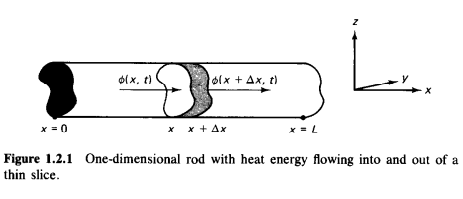
\includegraphics[width=0.7\textwidth]{media1/media/image2.png}
    \caption{Physical model of a one-dimensional rod showing heat energy flow into and out of a thin slice between $x$ and $x + \Delta x$. The heat flux entering at $x$ is denoted by $\phi(x,t)$ and the flux leaving at $x+\Delta x$ by $\phi(x+\Delta x,t)$.}
    \label{fig:heat_flow}
\end{figure}

\subhead{Fourier's Law of Heat Conduction}

According to \textbf{Fourier's Law}, the rate of heat flow $\heatflow_{x}$ (heat energy per unit time) through an area $A$ is proportional to the negative of the temperature gradient:

\begin{equation}
    \heatflow_{x} = - \thermcond A \pd{\temp}{x}
\end{equation}

where:

\noindent \textbf{SI Unit of} $\mathbf{\heatflow_{x}}$\textbf{:}
\begin{itemize}
    \item Heat energy = Joule (J)
    \item Time = second (s)
\end{itemize}

So:
\begin{equation}
    [\heatflow_{x}] = \frac{\text{J}}{\text{s}} = \text{Watt (W)}
\end{equation}

\noindent \textbf{Thermal conductivity $\thermcond$:} This constant tells how easily heat travels through a material. SI Unit of $\thermcond$:
\begin{equation}
    [\thermcond] = \frac{\text{W}}{\text{m}\cdot\text{K}}
\end{equation}

\noindent \textbf{SI units of Area $A$:}
\begin{equation}
    [A] = \text{m}^{2}
\end{equation}

\noindent \textbf{The temperature gradient} $\mathbf{\pd{\temp}{x}}$\textbf{:} This tells \textbf{how fast temperature changes} with distance. If $\temp$ changes rapidly $\rightarrow$ heat flows faster. \textbf{SI Units}:
\begin{itemize}
    \item Temperature = Kelvin (K)
    \item Distance = meter (m)
\end{itemize}

\begin{equation}
    \left[\pd{\temp}{x}\right] = \frac{\text{K}}{\text{m}}
\end{equation}

If temperature decreases along $+x$, the gradient is \textbf{negative.} The negative sign in Fourier's law forces heat to always flow \textbf{from higher temperature $\rightarrow$ lower temperature.}

\subhead{Heat Flow into and out of an Element}

Consider a small element of the rod between $x$ and $x + \Delta x$.

\begin{itemize}
    \item \textbf{Heat entering at $x$:} The heat flowing \textbf{INTO} the left face of the small rod element at position \textbf{$x$} is given by Fourier's law:
          \begin{equation}
              \heatflow_{x} = - \thermcond A \pd{\temp}{x}
          \end{equation}

    \item \textbf{Heat leaving at $x + \Delta x$:} At the right side of the element, the heat flow is \textbf{not exactly the same} because the temperature might change as we move from $\mathbf{x}$ \textbf{to} $\mathbf{x + \Delta x}$. So we evaluate Fourier's Law at $\mathbf{x + \Delta x}$:
\end{itemize}

\begin{equation}
    \heatflow_{x + \Delta x} = - \thermcond A\left( \pd{\temp}{x} \text{ evaluated at } x + \Delta x \right)
\end{equation}

Now we need to express:
\begin{equation*}
    \pd{\temp}{x}(x + \Delta x)
\end{equation*}
using a Taylor expansion. So,
\begin{equation}
    \pd{\temp}{x}(x + \Delta x) = \pd{\temp}{x}(x) + \pdd{\temp}{x}(x)\Delta x
\end{equation}

Substitute this expansion in the equation for $\heatflow_{x + \Delta x}$:
\begin{equation}
    \heatflow_{x + \Delta x} = - \thermcond A\left[ \pd{\temp}{x}(x) + \pdd{\temp}{x}(x)\Delta x \right]
\end{equation}

This is the \textbf{linear approximation} used for small $\Delta x$. Now compute the net heat inflow.

\begin{align*}
    \text{Net heat inflow} & = \text{Heat in} - \text{Heat out}         \\
                           & = \heatflow_{x} - \heatflow_{x + \Delta x}
\end{align*}

\begin{align}
    \heatflow_{x} - \heatflow_{x + \Delta x} & = - \thermcond A \pd{\temp}{x} - \left[ - \thermcond A\left( \pd{\temp}{x}(x) + \pdd{\temp}{x}(x)\Delta x \right) \right] \nonumber \\
                                             & = - \thermcond A \pd{\temp}{x} + \thermcond A \pd{\temp}{x} + \thermcond A\pdd{\temp}{x}\Delta x
\end{align}

Hence, \textbf{net rate of heat flow into the element}:
\begin{equation}
    \heatflow_{x} - \heatflow_{x + \Delta x} = \thermcond A\pdd{\temp}{x}\Delta x
\end{equation}

\subhead{Heat Energy Flow Rate (Storage Term)}

\textbf{Thermal Energy:} Every material contains \textbf{internal thermal energy}. When temperature increases, the internal energy increases. For \textbf{each kilogram of material}, the amount of energy needed to increase temperature by 1 Kelvin is \textbf{specific heat ($\specheat$).}

\textbf{SI units:} Joule per kilogram per kelvin $[\text{J}/(\text{kg}\cdot\text{K})]$.

If temperature changes by some amount $\Delta \temp$, the energy increase per kg is:
\begin{equation*}
    \specheat \times (\text{change in temperature})
\end{equation*}

\noindent \textbf{Mass of element:} We take a very small piece of the rod of cross-sectional area $A$ and length $\Delta x$. So the volume of the element is:
\begin{equation*}
    A \times \Delta x
\end{equation*}

The density $\density$ tells us how much mass is inside one cubic metre. \\
\textbf{SI units:} kilogram per cubic metre ($\text{kg/m}^{3}$).

So,
\begin{equation*}
    \text{Mass of element} = \density \times A \times \Delta x
\end{equation*}

\noindent \textbf{Energy stored in that mass:} Energy stored due to a temperature rise is:
\begin{equation*}
    \density A \Delta x \times \specheat \times (\text{change in temperature})
\end{equation*}

Temperature varies with time $\rightarrow$ so it changes \textbf{per second}. Rate of change of temperature with respect to time, at that location:
\begin{equation}
    \pd{\temp}{t}
\end{equation}
\textbf{SI units:} Kelvin per second (K/s).

So energy change per second (rate of increase of energy) is:
\begin{equation*}
    \density A \Delta x \times \specheat \times \pd{\temp}{t}
\end{equation*}

So, the rate of increase of thermal energy in the element (of volume $A\Delta x$) is:
\begin{equation}
    \text{Rate of energy storage} = \density \specheat A \Delta x \pd{\temp}{t}
\end{equation}

\subhead{Energy Balance}

\textbf{By Conservation of Energy:}\\
Net heat inflow + Heat generated = Rate of increase of energy

\noindent \textbf{Net heat Inflow:}
\begin{equation*}
    = \thermcond A\pdd{\temp}{x}\Delta x
\end{equation*}

\noindent \textbf{Heat generated inside the element:}\\
Let $q'''$ be the internal heat generation per unit volume and Volume of element $A\Delta x$. So heat generated inside element per second:
\begin{equation*}
    q''' \times A\Delta x
\end{equation*}

\noindent \textbf{Rate of increase of stored Thermal Energy:}\\
The rate at which its internal energy changes is:
\begin{equation*}
    \density \specheat A \Delta x \pd{\temp}{t}
\end{equation*}

This comes from the fact:
\begin{itemize}
    \item $\density = \text{density (kg per cubic metre)}$
    \item $A \times \Delta x = \text{volume (cubic metre)} \rightarrow \text{so mass} = \density A\Delta x$
    \item $\specheat = \text{specific heat (J per kg per K)}$
    \item $\pd{\temp}{t} = \text{rate of temperature change (K per second)}$
\end{itemize}

Multiplying the units,
\begin{equation*}
    \text{kg} \times \frac{\text{J}}{\text{kg}\cdot\text{K}} \times \frac{\text{K}}{\text{s}} = \frac{\text{J}}{\text{s}} \text{ (Joule per sec)}
\end{equation*}

This is the \textbf{rate at which thermal energy increases} inside the element.

Now substituting in the equation:
\begin{equation}
    \thermcond A\left( \pdd{\temp}{x} \right)\Delta x + q''' \times A\Delta x = \density \specheat A \Delta x \pd{\temp}{t}
\end{equation}

This is the \textbf{conservation of energy equation} applied to a tiny rod element.

Cancel $A\Delta x$ (since nonzero):
\begin{equation}
    \thermcond\pdd{\temp}{x} + q''' = \density \specheat\pd{\temp}{t}
\end{equation}

Now we have \textbf{no} $\Delta x$, meaning this holds at every point in the rod.

\subhead{General Heat Conduction Equation (1D Transient Form)}

\begin{equation}
    \pd{\temp}{t} = \thermdiff\pdd{\temp}{x} + \frac{q'''}{\density \specheat}
\end{equation}

Where $\thermdiff = \thermcond/\density \specheat$ is called the \textbf{thermal diffusivity} (m\textsuperscript{2}/s).

\subhead{Special Cases}

\noindent \textbf{(a) Steady-State Conduction (no time dependence):}
\begin{equation}
    \pd{\temp}{t} = 0 \implies \frac{d^{2}\temp}{dx^{2}} = - \frac{q'''}{\thermcond}
\end{equation}

\noindent \textbf{(b) No Internal Heat Generation:}
\begin{equation}
    \pd{\temp}{t} = \thermdiff\pdd{\temp}{x}
\end{equation}
or equivalently,
\begin{equation}
    \disp_{t} = \thermdiff \disp_{xx}
\end{equation}
This is the standard one-dimensional transient heat conduction equation.

\subhead{Extension to Two Dimension}

In a 2-D plate, heat flows in both $x$ and $y$ directions. Energy balance in a 2-D control area gives:
\begin{equation}
    \disp_{t} = \thermdiff\left( \disp_{xx} + \disp_{yy} \right)
\end{equation}
This is the 2-Dimensional Heat Equation.

\subhead{Laplace Equation}

At steady state, \textbf{temperature remains constant does not chnge with respect to time}, so:
\begin{equation*}
    \disp_{t} = 0
\end{equation*}

From the 2D heat equation:
\begin{equation}
    \disp_{xx} + \disp_{yy} = 0
\end{equation}

This forms the \textbf{Laplace Equation}. In general:
\begin{equation}
    \laplacian\disp = 0
\end{equation}

% ==========================================
\section{Wave Equation}
% ==========================================

The transverse vibration of a stretched elastic membrane (like a drumhead) is described by the wave equation. It's assumed that the membrane is thin, flexible and is stretched evenly, and that it has small vertical displacements. The derivation is derived from Newton's second law related to a differential membrane element. By analyzing the vertical components of tension forces, the governing partial differential equation is obtained. This equation describes the propagation of wave motion on the membrane.

\subhead{Physical Model: Vibrating Membrane}

We consider a thin, elastic, flexible membrane stretched tightly in the plane.

\noindent Examples:
\begin{itemize}
    \item A drumhead
    \item Thin elastic sheet
    \item Rubber membrane with uniform tension
\end{itemize}

Let:
\begin{itemize}
    \item $\disp(x,y,t)$ = vertical displacement of the membrane
    \item $(x,y)$ = coordinates in the membrane plane
    \item $t$ = time
\end{itemize}

Assumptions:
\begin{itemize}
    \item Displacements are small.
    \item Tension is uniform across the membrane.
    \item Membrane has mass per unit area $\density$.
    \item Only vertical motion is considered.
\end{itemize}

\subhead{Geometry of a Small Rectangular Element}

Consider a small \textbf{rectangular piece} of the membrane surface.

\noindent \textbf{Vertices at} $(x,y), (x + \Delta x,y), (x,y + \Delta y), (x + \Delta x,y + \Delta y)$
\begin{itemize}
    \item Starting corner: $(x,y)$
    \item Move right by a little distance $\Delta x$: $(x + \Delta x,y)$
    \item Move upward by a little distance $\Delta y$: $(x,y + \Delta y)$
    \item Opposite corner: $(x + \Delta x,y + \Delta y)$
\end{itemize}

\noindent \textbf{Area of tiny rectangle is} $\Delta S = \Delta x \, \Delta y$

\noindent \textbf{Tension Force:} Each side of the element is pulled by a tension force tangential to the membrane. Let $\tension$ = tension per unit length (constant). $\tension$ is the \textbf{force per unit length} along an edge. If an edge has length $\Delta y$, the total tension along the edge is:
\begin{equation*}
    \tension \cdot \Delta y
\end{equation*}

\noindent \textbf{Slope of membrane:} The slope of the membrane gives the vertical component of tension. If the membrane surface is described by $\disp(x,y,t)$, and $\disp$ = height above the $xy$-plane, the slope is the derivative of $\disp$. Then:
\begin{itemize}
    \item slope in $x$-direction: $\disp_{x}$
    \item slope in $y$-direction: $\disp_{y}$
\end{itemize}

\noindent \textbf{For small slopes:}
\begin{equation}
    \text{For small angles} \quad \sin\theta \approx \tan\theta \approx \theta
\end{equation}
But,
\begin{equation*}
    \tan\theta_{x} = \disp_{x}
\end{equation*}
So for small angles:
\begin{equation}
    \sin\theta_{x} \approx \disp_{x}
\end{equation}
Same for the $y$-direction:
\begin{equation}
    \sin\theta_{y} \approx \disp_{y}
\end{equation}

The vertical component of tension = $\tension \sin\theta$. Thus,
\begin{equation}
    \tension \sin\theta_{x} \approx \tension(\disp_{x})
\end{equation}

\subhead{Vertical Components of Tension Forces}

\subhead{Left and right edges (parallel to $y$-axis)}

\noindent \textbf{Vertical force on right edge at $(x + \Delta x)$:}
\begin{itemize}
    \item Edge length (in the $y$-direction) = $\Delta y$
    \item Tension per unit length = $\tension$
    \item The slope in the $x$-direction at that edge is $\disp_{x}(x + \Delta x,y,t)$.
\end{itemize}

For \textbf{small slopes}, the vertical component of tension along that edge is $\approx \tension \sin\theta_{x} \approx \tension(\disp_{x})$.\\
So the \textbf{total vertical force on the right edge} is:
\begin{equation*}
    \tension \, \disp_{x}(x + \Delta x,y,t) \, \Delta y
\end{equation*}

Similarly, \textbf{vertical force on left edge at $x$} is:
\begin{equation*}
    \tension \, \disp_{x}(x,y,t) \, \Delta y
\end{equation*}

\noindent \textbf{Net vertical force in $x$-direction} = (right edge) $-$ (left edge):
\begin{equation}
    F_{x} = \tension [\disp_{x}(x + \Delta x,y,t) - \disp_{x}(x,y,t)] \Delta y
\end{equation}

\noindent \textbf{Using mean value approximation (Taylor series):} We need to express $\disp_{x}(x + \Delta x) - \disp_{x}(x)$ in terms of the derivative at $x$. Use Taylor expansion about $x$:
\begin{equation*}
    \disp_{x}(x + \Delta x,y,t) = \disp_{x}(x,y,t) + \disp_{xx}(x,y,t)\Delta x + \mathcal{O}(\Delta x^{2})
\end{equation*}

For a small element, we \textbf{neglect the higher order term} $\mathcal{O}(\Delta x^{2})$, and we get:
\begin{equation}
    \disp_{x}(x + \Delta x,y,t) - \disp_{x}(x,y,t) \approx \disp_{xx}(x,y,t)\Delta x
\end{equation}

Substituting back into the equation for $F_{x}$:
\begin{equation*}
    F_{x} \approx \tension \left[ \disp_{xx}(x,y,t) \Delta x \right] \Delta y = \tension \, \disp_{xx}(x,y,t) \, \Delta x \Delta y
\end{equation*}

Thus, the $x$-direction force becomes:
\begin{equation}
    F_{x} = \tension \, \disp_{xx} \, \Delta x \Delta y
\end{equation}

\subhead{Top and bottom edges (parallel to $x$-axis)}

\noindent \textbf{Vertical force on top edge at $(y + \Delta y)$:}
\begin{itemize}
    \item Edge length (in the $x$-direction) = $\Delta x$
    \item Tension per unit length = $\tension$
    \item The slope in the $y$-direction at that edge is $\disp_{y}(x,y + \Delta y)$.
\end{itemize}

For \textbf{small slopes}, the vertical component of tension along that edge is $\approx \tension \sin\theta_{y} \approx \tension(\disp_{y})$.\\
So the \textbf{total vertical force on the top edge} is:
\begin{equation*}
    \tension [\disp_{y}(x,y + \Delta y,t)] \Delta x
\end{equation*}

Similarly, \textbf{vertical force on bottom edge at $y$} is:
\begin{equation*}
    \tension \, \disp_{y}(x,y,t) \, \Delta x
\end{equation*}

\noindent \textbf{Net vertical force in $y$-direction} = (top edge) $-$ (bottom edge):
\begin{equation}
    F_{y} = \tension [\disp_{y}(x,y + \Delta y,t) - \disp_{y}(x,y,t)] \Delta x
\end{equation}

\noindent \textbf{Using mean value approximation (Taylor series):} We need to express $\disp_{y}(y + \Delta y) - \disp_{y}(y)$ in terms of the derivative at $y$. Use Taylor expansion about $y$:
\begin{equation*}
    \disp_{y}(x,y + \Delta y,t) = \disp_{y}(x,y,t) + \disp_{yy}(x,y,t)\Delta y + \mathcal{O}(\Delta y^{2})
\end{equation*}

For a small element, we \textbf{neglect the higher order term} $\mathcal{O}(\Delta y^{2})$, and we get:
\begin{equation}
    \disp_{y}(x,y + \Delta y,t) - \disp_{y}(x,y,t) \approx \disp_{yy}(x,y,t)\Delta y
\end{equation}

Substituting back into the equation for $F_{y}$:
\begin{equation*}
    \tension \left[ \disp_{y}(x,y + \Delta y,t) - \disp_{y}(x,y,t) \right] \Delta x \approx \tension \disp_{yy} \, \Delta y \Delta x
\end{equation*}

Thus, the $y$-direction force becomes:
\begin{equation}
    F_{y} = \tension \, \disp_{yy} \, \Delta x \Delta y
\end{equation}

\subhead{Total Vertical Force}

Adding the force equations:
\begin{equation}
    F_{\text{vertical}} = \tension(\disp_{xx} + \disp_{yy}) \Delta x \Delta y
\end{equation}

\subhead{Apply Newton's Law}

By Newton's 2nd law ($F = ma$) with:
\begin{itemize}
    \item Mass of the element $m = \density \Delta x \Delta y$
    \item Vertical acceleration $a = \disp_{tt}(x,y,t)$
\end{itemize}
So we get:
\begin{equation}
    \tension(\disp_{xx} + \disp_{yy})\Delta x \Delta y = \density \Delta x \Delta y \, \disp_{tt}
\end{equation}

Cancel $\Delta x \Delta y$:
\begin{equation*}
    \tension(\disp_{xx} + \disp_{yy}) = \density \disp_{tt}
\end{equation*}
\begin{equation}
    \disp_{tt} = \frac{\tension}{\density}(\disp_{xx} + \disp_{yy})
\end{equation}

\subhead{Wave Speed}

Let:
\begin{equation*}
    \wavespeed = \sqrt{\frac{\tension}{\density}} \implies \wavespeed^{2} = \frac{\tension}{\density}
\end{equation*}

\noindent \textbf{SI units:}
$\tension = \frac{\text{N}}{\text{m}} = \text{kg}\cdot\text{s}^{-2}$ and $\density = \text{kg}\cdot\text{m}^{-2}$. Therefore:
\begin{equation*}
    \wavespeed^{2} = \text{m}^{2}\cdot\text{s}^{-2}
\end{equation*}

Hence the 2-D wave equation is:
\begin{equation}
    \mathbf{\disp_{tt} = \wavespeed^{2}\left( \disp_{xx} + \disp_{yy} \right)}
\end{equation}
or equivalently:
\begin{equation}
    \disp_{tt} = \wavespeed^{2}\laplacian\disp
\end{equation}
where $\laplacian\disp = \disp_{xx} + \disp_{yy}$.

This is the classical PDE for vibrating membranes (drumheads, elastic sheets).

\subhead{Laplace Equation}

If the membrane reaches a \textbf{steady-state configuration}, the shape of the surface no longer changes with time. Therefore,
\begin{equation}
    \disp_{tt} = 0
\end{equation}

Substituting into the wave equation:
\begin{equation*}
    0 = \wavespeed^{2}(\disp_{xx} + \disp_{yy})
\end{equation*}

Dividing by $\wavespeed^{2}$ gives the \textbf{Laplace equation}:
\begin{equation}
    \disp_{xx} + \disp_{yy} = 0
\end{equation}

% ==========================================
\section{Black--Scholes Equation}
% ==========================================

In mathematical finance, the Black–Scholes–Merton partial differential equation tracks derivative price evolution under the Black–Scholes model, and broadly represents similar equations used for diverse option pricing.

\subhead{Formula For Financial Interpretation}

\begin{equation}
    \pd{V}{t} + \frac{1}{2}\pdd{V}{s}\sigma^{2}s^{2} + Rs\pd{V}{s} - RV = 0
\end{equation}

The left-hand side consists of a ``time decay'' term, the change in derivative value with respect to time, called theta, and a term involving the second spatial derivative gamma, the convexity of the derivative value with respect to the underlying value. The right-hand side is the riskless return from a long position in the derivative and a short position consisting of $\pd{V}{s}$ shares of the underlying asset.

\subhead{Derivation}

Major components behind this model are:
\begin{itemize}
    \item Stochastic differential equation.
    \item Ito's Lemma.
    \item Delta Hedge Portfolio.
\end{itemize}

\subhead{Stochastic Differential Equation}

When a variable changes unpredictably over time, it is considered to follow a stochastic process. In financial markets, the efficient market theory suggests that stock prices appear to move randomly. Although there are different views, they generally agree on two main ideas:

\begin{enumerate}
    \item The current stock price reflects all past information.
    \item New information causes the market to react quickly.
\end{enumerate}

Based on these ideas, stock prices are modeled using a Markov process, where only the current value matters for predicting future changes. This leads to the stochastic differential equation that models the stock's value:

\begin{equation}
    \frac{ds}{s} = \mu dt + \sigma dX
\end{equation}

There are two components:
\begin{itemize}
    \item \textbf{Predictable deterministic component ($\mu dt$):} The parameter $\mu$ is drift; it is used to calculate the standard cost of growth of the asset value.
    \item \textbf{Random donations to the return ($\sigma dX$):} Here $\sigma$ is volatility and is used to measure the average deviation of return. The amount $dX$ is a random variable having a normal distribution with mean zero and variance $dt$.
\end{itemize}

\subhead{Ito's Lemma}

We require Ito's lemma, a variation of Taylor's theorem that applies to the variable with random function.

\noindent \textbf{Taylor series:} On an interval $I$, suppose $g$ be a function which is differentiable. Then the Taylor series of $g$ at $x = a$ is:
\begin{equation}
    \sum_{n = 0}^{\infty} \frac{g^{(n)}(a)}{n!}(x - a)^{n}
\end{equation}

Suppose the above series is convergent on $I$, then
\begin{align}
    g(x)        & = g(a) + \sum_{n = 1}^{\infty} \frac{g^{(n)}(a)}{n!}(x - a)^{n} \\
    g(x) - g(a) & = \sum_{n = 1}^{\infty} \frac{g^{(n)}(a)}{n!}(x - a)^{n}
\end{align}

Replacing $x$ with $x + \Delta x$ and $a$ with $x$ we get:
\begin{equation}
    \Delta g = g(x + \Delta x) - g(x) = g'(x)\Delta x + \frac{g''(x)}{2!}(\Delta x)^{2} + \dots
\end{equation}

This connects the tiny modification $\Delta g$ in the function $g$ to the tiny modification $\Delta x$ in $x$. We now move to thinking about what transpired to:
\begin{equation*}
    \frac{ds}{s} = \mu dt + \sigma dX
\end{equation*}

With probability 1, $(dX)^{2} \rightarrow dt$ as $t \rightarrow 0$.

Suppose that $g(y)$ is an asset value function of $V$. If we modify $y$ by some amount $dy$ then:
\begin{equation}
    dg = \frac{dg}{ds}ds + \frac{1}{2}\frac{d^{2}g}{ds^{2}}(ds)^{2} + \dots
\end{equation}

Now $ds = s(\mu dt + \sigma dX)$ and
\begin{equation*}
    (ds)^{2} = s^{2}\left( \mu^{2}(dt)^{2} + 2\mu\sigma dt\, dX + \sigma^{2}(dX)^{2} \right)
\end{equation*}

Now since $(dX)^{2} \rightarrow dt$ as $t \rightarrow 0$, the term $s^{2}\sigma^{2}(dX)^{2}$ becomes $s^{2}\sigma^{2}dt$, which remains for the above terms for $(ds)^{2}$ as $dt$ is very small. So,
\begin{equation*}
    (ds)^{2} \approx s^{2}\sigma^{2}dt
\end{equation*}

As an estimate for $(ds)^{2}$ as $dt \rightarrow 0$, we have:
\begin{equation}
    dg = \frac{dg}{ds}ds + \frac{1}{2}\frac{d^{2}g}{ds^{2}}(s^{2}\sigma^{2}dt)
\end{equation}
\begin{equation*}
    dg = \frac{dg}{ds}(s\mu dt + s\sigma dX) + \frac{1}{2}\frac{d^{2}g}{ds^{2}}(s^{2}\sigma^{2}dt)
\end{equation*}
\begin{equation}
    dg = \sigma s \frac{dg}{ds}dX + \left( \mu s \frac{dg}{ds} + \frac{1}{2}\frac{d^{2}g}{ds^{2}}s^{2}\sigma^{2} \right)dt
\end{equation}

Ito's Lemma explains how a minor change in a function depends on both the random movement of a variable and the regular passage of time. Since a stochastic process has a random part and a deterministic part, Ito's Lemma connects these to show how a function of such a variable changes. For a function with two variables, $g(s,t)$, Ito's Lemma gives:

\begin{equation}
    dg = \sigma s \pd{g}{s}dX + \left( \mu s \pd{g}{s} + \frac{1}{2}\pdd{g}{s}\sigma^{2}s^{2} + \pd{g}{t} \right)dt
\end{equation}

This equation shows how the cost of an option changes over time as a stock price function.

\subhead{Delta Hedge Portfolio}

\begin{equation}
    \Pi = V - \Delta s
\end{equation}

The probability of an option's expiration date is known as the delta hedge. Delta hedging reduces the risk from movements in the underlying asset by adjusting the position using the option's delta. The idea is to keep the portfolio neutral to price changes.

\subhead{The Black-Scholes PDE}

Suppose the price of an option is $V(s,t)$ and the rate of interest be $R$ and $\mu$ (drift) and $\sigma$ (Volatility) as used above. By Ito's Lemma we get:

\begin{equation}
    dV = \sigma s \pd{V}{s}dX + \left( \mu s \pd{V}{s} + \frac{1}{2}\pdd{V}{s}\sigma^{2}s^{2} + \pd{V}{t} \right)dt
\end{equation}

Consider the portfolio having a single option and $-\Delta$ units of the stock. The cost of the portfolio is:
\begin{equation}
    \Pi = V - \Delta s
\end{equation}

So,
\begin{align*}
    d\Pi & = dV - \Delta ds                                                                                                                                  \\
    d\Pi & = \sigma s \pd{V}{s}dX + \left( \mu s \pd{V}{s} + \frac{1}{2}\pdd{V}{s}\sigma^{2}s^{2} + \pd{V}{t} \right)dt - \Delta s\mu dt - \Delta s\sigma dX \\
    d\Pi & = \sigma s\left( \pd{V}{s} - \Delta \right)dX + \left( \mu s \pd{V}{s} + \frac{1}{2}\pdd{V}{s}\sigma^{2}s^{2} + \pd{V}{t} - \Delta s\mu \right)dt
\end{align*}

Choose $\Delta = \pd{V}{s}$ to get:
\begin{equation}
    d\Pi = \left( \frac{1}{2}\pdd{V}{s}\sigma^{2}s^{2} + \pd{V}{t} \right)dt
\end{equation}

So, suppose $\Pi$ was invested in without risk assets it would see a growth of $R\Pi dt$ in the interval length $dt$. Then for a fair value, we have:
\begin{equation}
    R\Pi dt = \left( \frac{1}{2}\pdd{V}{s}\sigma^{2}s^{2} + \pd{V}{t} \right)dt
\end{equation}

Substitute $\Pi = V - \pd{V}{s}s$:
\begin{equation}
    R\left( V - \pd{V}{s}s \right) = \frac{1}{2}\pdd{V}{s}\sigma^{2}s^{2} + \pd{V}{t}
\end{equation}

Rearranging terms gives:
\begin{equation}
    \boxed{ \pd{V}{t} + \frac{1}{2}\pdd{V}{s}\sigma^{2}s^{2} + Rs\pd{V}{s} - RV = 0 }
\end{equation}

The above equation is the \textbf{``Black-Scholes Partial Differential Equation''}.

% ========================================== o
\chapter{Numerical Methods}
% ==========================================
Most Partial Differential Equations (PDEs) do not have analytical solutions. If we cannot find exact solutions we resort to Numerical Methods. Using these methods breaks a domain of continuous problems down into discrete steps and thus calculates for high accuracy of approximation. They are important in fields like engineering, physics and finance, where not all problems have precise solutions and involve problems of a more complex nature.

One such important method for computing derivatives is the Finite Difference Method (FDM). As opposed to solving the calculus directly, FDM numerically approximates these derivatives algebraically using values at certain points on the grid. This change makes it possible to solve the systems of linear or nonlinear algebraic equations, which computers can solve easily, instead of the differential equations.

The basic idea of FDM is to break up the domain into a structured grid or mesh. We then approximate the solution at these particular intersection points by substituting derivatives with finite difference approximations. Commonly resorted are the Forward differences, Backward differences or Central differences depending on the direction of the calculation.

Finite Difference Method (FDM) is one of the most popular techniques for regular and structured domains, with others including Finite Element Method (FEM), Finite Volume Method (FVM), and Spectral Methods. It is popular because it has a quick set-up, is easy to program, and requires minimal computing. The right step size yields excellent balance between speed and accuracy and is thus very useful for time-dependent problems in engineering and finance.

The Finite Difference Method is adopted in this study because of its simplicity, efficiency and its natural suitability for structured grid. FDM approach is suitable for direct discretization of our governing equations and gives us a clear pathway for checking FDM stability, convergence and accuracy. This is extremely suitable for engineering numerical simulation and financial mathematics.
\section{Finite Difference Methods}

The finite difference method (FDM) is a numerical solution to estimate the differentials of a differential equation. This approach is essentially replacing the concept of continuous derivatives with algebraic expressions based on values of the functions over discrete locations. Consequently, it can be solved by numerical methods and the differential equation will become a set of linear or nonlinear algebraic equations.

The approach starts with a discrete set of points (grid) over the space being computed. The values of the functions are estimated at these grid points and the derivatives are substituted with finite difference formulas. Examples of the many finite difference schemes used are:
\begin{itemize}
\item Forward Difference Method
\item Backward Difference Method
\item Central Difference Method
\end{itemize}


% ------------------------------------------
\subsection{Finite Difference Approximations for ODE's}
% ------------------------------------------

The Finite difference methods approximates derivatives using function values at nearby mesh points of a discrete mesh. Assume a smooth function $\disp(x)$ and a uniform mesh with step size $h$. Let grid points be:
\begin{equation*}
    x_{i - 1} = x_{i} - h, \quad \quad x_{i}, \quad \quad x_{i + 1} = x_{i} + h
\end{equation*}

now we derive approximations for the first derivative $\disp'(x)$ and second derivative $\disp''(x)$ using Taylor series expansions.

For a smooth function $\disp(x)$, expand about $x = x_{i}$:
\begin{align}
    \disp_{i + 1} & \equiv \disp(x_{i} + h) = \disp_{i} + h\disp_{i}' + \frac{h^{2}}{2} \disp_{i}'' + \frac{h^{3}}{6} \disp_{i}^{(3)} + \frac{h^{4}}{24}\disp_{i}^{(4)} + \dots \\
    \disp_{i - 1} & \equiv \disp(x_{i} - h) = \disp_{i} - h\disp_{i}' + \frac{h^{2}}{2}\disp_{i}'' - \frac{h^{3}}{6}\disp_{i}^{(3)} + \frac{h^{4}}{24}\disp_{i}^{(4)} - \dots
\end{align}

\subhead{Forward Difference Approximation (1\textsuperscript{st} Derivative)}

The Taylor expansion of $\disp(x_{i} + h)$ about $x$ is:
\begin{equation}
    \disp_{i + 1} \equiv \disp(x_{i} + h) = \disp_{i} + h\disp_{i}' + \frac{h^{2}}{2} \disp_{i}'' + \frac{h^{3}}{6} \disp_{i}^{(3)} + \frac{h^{4}}{24}\disp_{i}^{(4)} + \dots
\end{equation}

Rearranging for the first derivative:
\begin{equation*}
    \disp'(x_{i}) = \frac{\disp_{i + 1} - \disp_{i}}{h} - \frac{h}{2} \disp_{i}'' - \frac{h^{2}}{6} \disp_{i}^{(3)} - \dots
\end{equation*}

Neglecting higher-order terms yields the \textbf{forward difference approximation}:
\begin{equation}
    \disp'(x_{i}) \approx \frac{\disp_{i + 1} - \disp_{i}}{h}
\end{equation}

\textbf{Accuracy:} The leading error term is $- \frac{h}{2} \disp''(x)$, so this approximation is \textbf{first-order accurate, $\mathcal{O}(h)$}.

\subhead{Forward Difference (2\textsuperscript{nd} Derivative)}

We want an approximation of $\disp''(x_{i})$ using $\disp_{i}, \disp_{i + 1}, \disp_{i + 2}$. Use Taylor expansions at $(x_{i} + h)$ and $(x_{i} + 2h)$:
\begin{align}
    \disp_{i + 1} & = \disp(x_{i} + h) = \disp_{i} + h\disp'_{i} + \frac{h^{2}}{2}\disp_{i}'' + \frac{h^{3}}{6}\disp_{i}^{(3)} + \frac{h^{4}}{24}\disp_{i}^{(4)} + \mathcal{O}(h^{5}),                     \\
    \disp_{i + 2} & = \disp(x_{i} + 2h) = \disp_{i} + 2h\disp'_{i} + \frac{(2h)^{2}}{2}\disp''_{i} + \frac{(2h)^{3}}{6}\disp_{i}^{(3)} + \frac{(2h)^{4}}{24}\disp_{i}^{(4)} + \mathcal{O}(h^{5}) \nonumber \\
                  & = \disp_{i} + 2h\disp'_{i} + 2h^{2}\disp''_{i} + \frac{4}{3}h^{3}\disp_{i}^{(3)} + \frac{2}{3}h^{4}\disp_{i}^{(4)} + \mathcal{O}(h^{5}).
\end{align}

Eliminate the first derivative $\disp_{i}'$ by forming a linear combination and take $\disp_{i + 2} - 2\disp_{i + 1} + \disp_{i}$. Compute:
\begin{align*}
    \disp_{i + 2} - 2\disp_{i + 1} + \disp_{i} & = \left( \disp_{i} + 2h^{2}\disp_{i}'' + \frac{4}{3}h^{3}\disp_{i}^{(3)} + \frac{2}{3}h^{4}\disp_{i}^{(4)} \right)                                                                           \\
                                               & \quad - 2\left( h\disp'_{i} + \frac{h^{2}}{2}\disp_{i}'' + \frac{h^{3}}{6}\disp_{i}^{(3)} + \frac{h^{4}}{24}\disp_{i}^{(4)} \right) + (\disp_{i}) + \mathcal{O}(h^{5})                       \\
                                               & = (2h^{2} - h^{2})\disp_{i}'' + \left( \frac{4}{3}h^{3} - \frac{2}{6}h^{3} \right) \disp_{i}^{(3)} + \left( \frac{2}{3}h^{4} - \frac{2}{24}h^{4} \right)\disp_{i}^{(4)} + \mathcal{O}(h^{5}) \\
                                               & = h^{2}\disp_{i}'' + h^{3}\left( \frac{4}{3} - \frac{1}{3} \right) \disp_{i}^{(3)} + h^{4}\left( \frac{2}{3} - \frac{1}{12} \right)\disp_{i}^{(4)} + \mathcal{O}(h^{5})                      \\
                                               & = h^{2}\disp_{i}'' + h^{3}\disp_{i}^{(3)} + \frac{7}{12}h^{4}\disp_{i}^{(4)} + \mathcal{O}(h^{5}).
\end{align*}

Therefore,
\begin{equation}
    \disp_{i}'' = \frac{\disp_{i + 2} - 2\disp_{i + 1} + \disp_{i}}{h^{2}} - h\disp_{i}^{(3)} - \frac{7}{12}h^{2}\disp_{i}^{(4)} + \mathcal{O}(h^{3})
\end{equation}

Dropping higher derivatives yields the forward two-step second derivative:
\begin{equation}
    \disp''_{i} \approx \frac{\disp_{i + 2} - 2\disp_{i + 1} + \disp_{i}}{h^{2}} \quad \text{with leading truncation error } \mathcal{O}(h).
\end{equation}

\subhead{Backward Difference Approximation (1\textsuperscript{st} Derivative)}

Take the Taylor expansion of $\disp(x_{i} - h)$:
\begin{equation}
    \disp_{i - 1} \equiv \disp(x_{i} - h) = \disp_{i} - h\disp_{i}' + \frac{h^{2}}{2}\disp_{i}'' - \frac{h^{3}}{6}\disp_{i}^{(3)} + \frac{h^{4}}{24}\disp_{i}^{(4)} - \dots
\end{equation}

Rearranging:
\begin{equation*}
    \disp'(x_{i}) = \frac{\disp_{i} - \disp_{i - 1}}{h} + \frac{h}{2}\disp_{i}'' - \frac{h^{2}}{6}\disp_{i}^{(3)} + \dots
\end{equation*}

Neglecting smaller terms gives the \textbf{backward difference approximation}:
\begin{equation}
    \disp'(x_{i}) \approx \frac{\disp_{i} - \disp_{i - 1}}{h}
\end{equation}

\textbf{Accuracy:} Error term is again proportional to $h$, so it is \textbf{first-order accurate, $\mathcal{O}(h)$.}

\subhead{Backward Difference (2\textsuperscript{nd} Derivative)}

We want an approximation of $\disp''(x_{i})$ using $\disp_{i}, \disp_{i - 1}, \disp_{i - 2}$. Use Taylor expansions at $(x_{i} - h)$ and $(x_{i} - 2h)$ about $x_{i}$:
\begin{align}
    \disp_{i - 1} & = \disp_{i} - h\disp'_{i} + \frac{h^{2}}{2}\disp''_{i} - \frac{h^{3}}{6}\disp_{i}^{(3)} + \frac{h^{4}}{24}\disp_{i}^{(4)} + \mathcal{O}(h^{5}), \\
    \disp_{i - 2} & = \disp_{i} - 2h\disp'_{i} + 2h^{2}\disp''_{i} - \frac{4}{3}h^{3}\disp_{i}^{(3)} + \frac{2}{3}h^{4}\disp_{i}^{(4)} + \mathcal{O}(h^{5}).
\end{align}

Eliminate the first derivative $\disp_{i}'$ by forming a linear combination. Form $\disp_{i} - 2\disp_{i - 1} + \disp_{i - 2}$ to get:
\begin{equation*}
    \disp_{i} - 2\disp_{i - 1} + \disp_{i - 2} = h^{2}\disp''_{i} - h^{3}\disp_{i}^{(3)} + \frac{7}{12}h^{4}\disp_{i}^{(4)} + \mathcal{O}(h^{5}).
\end{equation*}
\begin{equation}
    \disp''_{i} = \frac{\disp_{i} - 2\disp_{i - 1} + \disp_{i - 2}}{h^{2}} + h \disp_{i}^{(3)} - \frac{7}{12}h^{2}\disp_{i}^{(4)} + \mathcal{O}(h^{3}).
\end{equation}

Dropping higher derivatives, the backward approximation for the second derivative is:
\begin{equation}
    \disp''_{i} \approx \frac{\disp_{i} - 2\disp_{i - 1} + \disp_{i - 2}}{h^{2}} \quad \text{with truncation error } \mathcal{O}(h).
\end{equation}

\subhead{Central Difference Approximation (1\textsuperscript{st} Derivative)}

Using Taylor expansions of $\disp(x_{i} + h)$ and $\disp(x_{i} - h)$:
\begin{align}
    \disp_{i + 1} & \equiv \disp(x_{i} + h) = \disp_{i} + h\disp_{i}' + \frac{h^{2}}{2} \disp_{i}'' + \frac{h^{3}}{6} \disp_{i}^{(3)} + \frac{h^{4}}{24}\disp_{i}^{(4)} + \dots \\
    \disp_{i - 1} & \equiv \disp(x_{i} - h) = \disp_{i} - h\disp_{i}' + \frac{h^{2}}{2}\disp_{i}'' - \frac{h^{3}}{6}\disp_{i}^{(3)} + \frac{h^{4}}{24}\disp_{i}^{(4)} - \dots
\end{align}

Subtracting:
\begin{equation*}
    \disp_{i + 1} - \disp_{i - 1} = 2h\disp_{i}' + \frac{2h^{3}}{6} \disp_{i}^{(3)} + \dots
\end{equation*}

Solving for the derivative:
\begin{equation*}
    \disp'(x_{i}) = \frac{\disp_{i + 1} - \disp_{i - 1}}{2h} - \frac{h^{2}}{6} \disp_{i}^{(3)} - \dots
\end{equation*}

Neglecting higher-order terms yields the \textbf{central difference approximation}:
\begin{equation}
    \disp'(x_{i}) \approx \frac{\disp_{i + 1} - \disp_{i - 1}}{2h}
\end{equation}

\textbf{Accuracy:} The leading error term is proportional to $h^{2}$, making this scheme \textbf{second-order accurate, $\mathcal{O}(h^{2})$}.

\subhead{Central Difference (2\textsuperscript{nd} Derivative)}

Using Taylor expansions of $\disp(x_{i} + h)$ and $\disp(x_{i} - h)$:
\begin{align}
    \disp_{i + 1} & \equiv \disp(x_{i} + h) = \disp_{i} + h\disp_{i}' + \frac{h^{2}}{2} \disp_{i}'' + \frac{h^{3}}{6} \disp_{i}^{(3)} + \frac{h^{4}}{24}\disp_{i}^{(4)} + \dots \\
    \disp_{i - 1} & \equiv \disp(x_{i} - h) = \disp_{i} - h\disp_{i}' + \frac{h^{2}}{2}\disp_{i}'' - \frac{h^{3}}{6}\disp_{i}^{(3)} + \frac{h^{4}}{24}\disp_{i}^{(4)} - \dots
\end{align}

Adding:
\begin{equation*}
    \disp_{i + 1} + \disp_{i - 1} = 2\disp_{i} + h^{2}\disp_{i}'' + \frac{h^{4}}{12}\disp_{i}^{(4)} + \dots
\end{equation*}

Rearranging:
\begin{equation*}
    \disp''(x_{i}) = \frac{\disp_{i + 1} - 2\disp_{i} + \disp_{i - 1}}{h^{2}} - \frac{h^{2}}{12}\disp^{(4)}(x_{i}) - \dots
\end{equation*}

Neglecting smaller terms gives the widely used central second-derivative approximation:
\begin{equation}
    \disp''(x_{i}) \approx \frac{\disp_{i + 1} - 2\disp_{i} + \disp_{i - 1}}{h^{2}}
\end{equation}

\textbf{Accuracy:} This approximation is \textbf{second-order accurate, $\mathcal{O}(h^{2})$}.

% ------------------------------------------
\subsection{Finite Difference Approximations for PDE's}
% ------------------------------------------

The continuous spatial domain is discretized into a finite grid in order to find numerical solutions of partial differential equations. Finite difference formulas are then used to approximate the partial derivatives of the unknown function with respect to spatial variables. Let
\begin{equation*}
    \disp = \disp(x,y)
\end{equation*}
with grid points
\begin{equation*}
    x_{i} = x_{0} + ih, \quad \quad y_{j} = y_{0} + jk
\end{equation*}
And
\begin{equation*}
    \disp_{i,j} = \disp(x_{i},y_{j})
\end{equation*}

\subhead{First Derivatives}

The general finite difference approximations for first-order partial derivatives are given as follows:

\noindent \textbf{Forward difference}
\begin{align}
    \pd{\disp}{x} & \approx \frac{\disp_{i + 1,j} - \disp_{i,j}}{h} \\
    \pd{\disp}{y} & \approx \frac{\disp_{i,j + 1} - \disp_{i,j}}{k}
\end{align}

\noindent \textbf{Backward difference}
\begin{align}
    \pd{\disp}{x} & \approx \frac{\disp_{i,j} - \disp_{i - 1,j}}{h} \\
    \pd{\disp}{y} & \approx \frac{\disp_{i,j} - \disp_{i,j - 1}}{k}
\end{align}

\noindent \textbf{Central difference}
\begin{align}
    \pd{\disp}{x} & \approx \frac{\disp_{i + 1,j} - \disp_{i - 1,j}}{2h} \\
    \pd{\disp}{y} & \approx \frac{\disp_{i,j + 1} - \disp_{i,j - 1}}{2k}
\end{align}

\subhead{Second Derivatives}

The general finite difference approximations for second-order partial derivatives are given as follows:

\noindent \textbf{Forward difference}
\begin{align}
    \pdd{\disp}{x} & \approx \frac{\disp_{i + 2,j} - 2\disp_{i + 1,j} + \disp_{i,j}}{h^{2}} \\
    \pdd{\disp}{y} & \approx \frac{\disp_{i,j + 2} - 2\disp_{i,j + 1} + \disp_{i,j}}{k^{2}}
\end{align}

\noindent \textbf{Backward difference}
\begin{align}
    \pdd{\disp}{x} & \approx \frac{\disp_{i,j} - 2\disp_{i - 1,j} + \disp_{i - 2,j}}{h^{2}} \\
    \pdd{\disp}{y} & \approx \frac{\disp_{i,j} - 2\disp_{i,j - 1} + \disp_{i,j - 2}}{k^{2}}
\end{align}

\noindent \textbf{Central difference}
\begin{align}
    \pdd{\disp}{x} & \approx \frac{\disp_{i + 1,j} - 2\disp_{i,j} + \disp_{i - 1,j}}{h^{2}} \\
    \pdd{\disp}{y} & \approx \frac{\disp_{i,j + 1} - 2\disp_{i,j} + \disp_{i,j - 1}}{k^{2}}
\end{align}

\chapter{Numerical Solutions for Advection or Wave Equation}
% ==========================================

This chapter presents the findings from the numerical techniques used to examine the behavior of the wave equation and the advection equation. The numerical solution of the Advection/Wave Equation using finite difference techniques is the primary topic of this presentation. The behavior of the solutions under various numerical schemes and conditions is examined using these techniques.

The numerical methods discussed in this chapter include:

\begin{itemize}
\item FTCS (Forward Time Centered Space) Method
\item Lax Method
\item Staggered Leapfrog Method
\end{itemize}

These methods are used to both Advection and the Wave Equation to examine several important properties, such as:

\begin{itemize}
\item Stability
\item Accuracy
\item Numerical diffusion
\item Oscillations
\item Convergence behavior
\end{itemize}

The comparison of these methods helps in understanding their strengths as well as some of their limitations, although the performance may vary depending on the problem being considered.

% ==========================================
\section{Advection Equation}
% ==========================================

Advection Equation is the simplest yet very important partial differential equations used for modeling wave propagation and transport phenomena. It describes how a physical quantity is transported with a constant velocity through space and time. Because of its simple mathematical form, it is often used as a basic model for testing and analyzing numerical methods, though the numerical behavior can sometimes become difficult to handle.

The one-dimensional advection equation is:

\begin{equation}
    \pd{\disp}{t} + \wavespeed\pd{\disp}{x} = 0
\end{equation}

Where:
\begin{itemize}
    \item ($\disp(x,t)$) represents the wave amplitude or transported quantity
    \item ($\wavespeed$) is the propagation velocity
    \item ($x$) is the spatial coordinate
    \item ($t$) is time
\end{itemize}

The equation describes the motion of a wave without changing its shape.

\subhead{Physical Interpretation}

The advection equation models pure transport. Examples include:
\begin{itemize}
    \item Motion of water waves
    \item Propagation of signals
    \item Transport of pollutants in air or water
    \item Traffic flow models
    \item Transport of heat by moving fluids
\end{itemize}

If the velocity ($\wavespeed > 0$), the wave moves toward the positive $x$-direction. \\
If the velocity ($\wavespeed < 0$), the wave moves toward the negative $x$-direction.

The shape of the wave ideally remains unchanged during propagation.

\subhead{Gaussian Initial Condition}

To study the propagation of waves, a Gaussian initial pulse is often used. The Gaussian initial condition is:
\begin{equation}
    \disp(x,0) = \frac{1}{\sqrt{2\pi}}e^{\frac{-x^{2}}{2}}
\end{equation}

This represents a smooth bell-shaped pulse centered around the origin. The Gaussian profile is useful because:
\begin{itemize}
    \item it is smooth and continuous
    \item it has finite amplitude
    \item it is mathematically convenient
    \item it clearly shows wave propagation behavior
\end{itemize}

In the advection equation, the Gaussian pulse moves without changing its shape.

\subhead{Similarity Solution Technique for the Advection Equation}

The similarity solution technique is used to reduce a PDE into an ODE.

For the advection equation:
\begin{equation*}
    \pd{\disp}{t} + \wavespeed\pd{\disp}{x} = 0
\end{equation*}

We noticed that solution moves with constant velocity ($\wavespeed$). This recommends that the solution depends on the combination:
\begin{equation}
    \xi = x - \wavespeed t
\end{equation}

Where:
\begin{equation*}
    \disp(x,t) = U(\xi)
\end{equation*}

The variable $\xi$ is known as similarity variable.

\subhead{Derivation of the Similarity Solution}

Assume:
\begin{equation*}
    \disp(x,t) = U(\xi)
\end{equation*}
With
\begin{equation*}
    \xi = x - \wavespeed t
\end{equation*}

Using the chain rule:

\noindent \textbf{Derivative with respect to time:}
\begin{equation*}
    \pd{\disp}{t} = \frac{dU}{d\xi}\pd{\xi}{t}
\end{equation*}
Since:
\begin{equation*}
    \pd{\xi}{t} = - \wavespeed
\end{equation*}
Therefore:
\begin{equation}
    \pd{\disp}{t} = - \wavespeed U'(\xi)
\end{equation}

\noindent \textbf{Derivative with respect to space:}
\begin{equation*}
    \pd{\disp}{x} = \frac{dU}{d\xi}\pd{\xi}{x}
\end{equation*}
Since:
\begin{equation*}
    \pd{\xi}{x} = 1
\end{equation*}
Therefore:
\begin{equation}
    \pd{\disp}{x} = U'(\xi)
\end{equation}


putting into the advection equation:
\begin{equation*}
    - \wavespeed U'(\xi) + \wavespeed U'(\xi) = 0
\end{equation*}
this simplifies to:
\begin{equation*}
    0 = 0
\end{equation*}

It shows that this form of any function :
\begin{equation}
    \disp(x,t) = f(x - \wavespeed t)
\end{equation}
which is the solution of the advection equation.

\subhead{Gaussian Solution of the Advection Equation}

Using the Gaussian initial condition:
\begin{equation*}
    \disp(x,0) = \frac{1}{\sqrt{2\pi}}e^{\frac{-x^{2}}{2}}
\end{equation*}

Replace $x$ by $(x - \wavespeed t)$:
\begin{equation}
    \disp(x,t) = \frac{1}{\sqrt{2\pi}}e^{\frac{-(x - \wavespeed t)^{2}}{2}}
\end{equation}

This shows a Gaussian pulse travels with velocity ($\wavespeed$) without changing its shape.

% ==========================================
\section{Finite Difference Method Approach}
% ==========================================

Analytical solutions are not always applicable for complex PDEs. Numerical methods approximate the solution on discrete mesh points. The domain is divided into small intervals of time and space.

\subhead{Space discretization}
\begin{equation*}
    x_{i} = i\Delta x
\end{equation*}

\subhead{Time discretization}
\begin{equation*}
    t^{n} = n\Delta t
\end{equation*}

The solution's numerical approximation is presented as:
\begin{equation*}
    \disp_{i}^{n} = \disp(x_{i},t^{n})
\end{equation*}

Where:
\begin{itemize}
    \item ($i$)  is for spatial index
    \item ($n$) is for the time level
\end{itemize}

\subhead{Finite Difference Approximations}

Finite difference approximations are used instead of the actual derivatives within the PDE.

\noindent \textbf{Forward Difference in Time:}
\begin{equation}
    \pd{\disp}{t} \approx \frac{\disp_{i}^{n + 1} - \disp_{i}^{n}}{\Delta t}
\end{equation}

\noindent \textbf{Centered Difference in Space:}
\begin{equation}
    \pd{\disp}{x} \approx \frac{\disp_{i + 1}^{n} - \disp_{i - 1}^{n}}{2\Delta x}
\end{equation}

% ==========================================
\section{FTCS Method}
% ==========================================

FTCS means:
\begin{itemize}
    \item Forward Time
    \item Centered Space
\end{itemize}

It uses:
\begin{itemize}
    \item forward difference formula in time
    \item centered difference formula in space
\end{itemize}

Applying these formula approximations to the advection equation:
\begin{equation*}
    \pd{\disp}{t} + \wavespeed\pd{\disp}{x} = 0
\end{equation*}

We obtain:
\begin{equation*}
    \frac{\disp_{i}^{n + 1} - \disp_{i}^{n}}{\Delta t} + \wavespeed\frac{\disp_{i + 1}^{n} - \disp_{i - 1}^{n}}{2\Delta x} = 0
\end{equation*}

Rearranging:
\begin{equation}
    \disp_{i}^{n + 1} = \disp_{i}^{n} - \frac{\wavespeed\Delta t}{2\Delta x}(\disp_{i + 1}^{n} - \disp_{i - 1}^{n})
\end{equation}

\subhead{Properties of FTCS Method}

Advantages:
\begin{itemize}
\item It is simple in implementation.
\item It is an explicit method.
\item Computaionally fast.
\end{itemize}

Disadvantages:
\begin{itemize}
\item It is unstable when used for advection equation.
\item Numerical oscillations increases with time.
\item Errors amplified fastly.
\end{itemize}

FTCS method is unconditionally unstable for advection equation.

\subhead{Instability in FTCS Method}

Instability occurs because centered spatial differences do not provide any numerical damping. Minor errors caused because of:
\begin{itemize}
\item the truncation errors
\item the rounding errors
\item the approximation errors
\end{itemize}
they are just keep growing while the time evolves.

This gives the results in:
\begin{itemize}
\item high oscillations
\item wave getting distorted
\item the solution is diverging
\end{itemize}

\subhead{Numerical Results and Graphical Interpretation: FTCS Method}

In MATLAB we used the finite difference scheme for the FTCS to model the advection equation. The next graphs illustrate the behavior of the FTCS method and its loss of stability during the propagation of the wave.

\noindent \textbf{FTCS Method ($c = 1$)}

This is the graph of the numerical solution of the advection equation using the FTCS method for $c = 1$.

\begin{figure}[H]
\centering
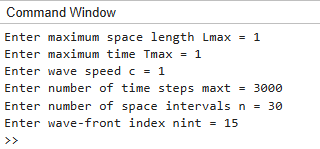
\includegraphics[width=0.45\textwidth]{media2/media/image1.png}
\quad

\includegraphics[width=0.35\textwidth]{media2/media/image2.png}
\caption{MATLAB inputs and the calculated CFL number for the FTCS method at wave speed $c = 1$.}
\label{fig:your_label_name}
\end{figure}

This 3D surface plot (Figure 5.2) displays the propagation of the wave amplitude as it travels both in space and time. In the beginning, the profile of the wave appears as though it's smooth, and looks right; after a time, however, you begin to see these irregular oscillations in the numerical solution. The graph is very exaggerated. The numerical solution cannot maintain the original wave shape, but will simply continue to grow in an uncontrollable manner.

This instability occurs because the linear advection equation is unconditionally unstable when using the FTCS method. Numerical errors are stored and amplified at each step. Because of this:
\begin{itemize}
\item oscillations increase with time goes on,
\item the solution becomes non-physical,
\item and the wave profile can not remains accurate.
\end{itemize}

\begin{figure}[H]
\centering
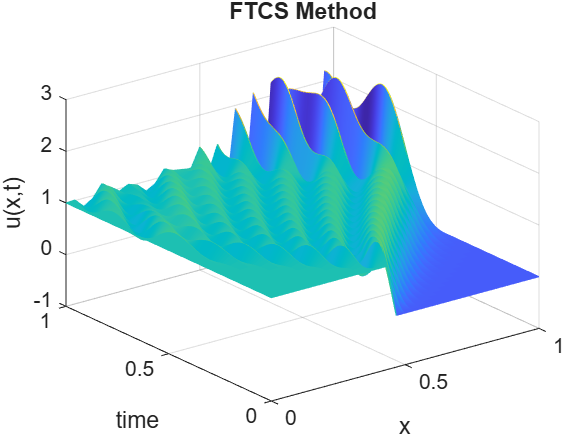
\includegraphics[width=0.45\textwidth]{media2/media/image3.png}
\quad
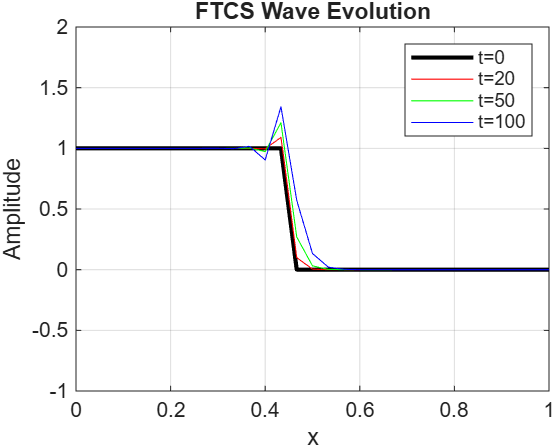
\includegraphics[width=0.45\textwidth]{media2/media/image4.png}
\caption{2D and 3D graphs showing unstable wave propagation and amplitude growth from truncation error with $c = 1$.}
\label{fig:your_label_name}
\end{figure}

The output of the FTCS method is not stable as can be seen in Figure 5.2. The oscillations that you are seeing near the wave front are due to the errors being exaggerated with each truncation. This results in oscillatory non-uniform solutions in the FTCS method of the advection equation.

\noindent \textbf{FTCS Method ($c = 2$)}

The results are from the FTCS method applied to the advection equation using a $c = 2$. In this, these are the graphs that illustrate the effect of increasing the CFL number.

\begin{figure}[H]
\centering
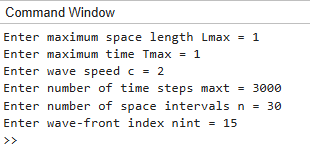
\includegraphics[width=0.45\textwidth]{media2/media/image5.png}
\quad
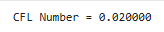
\includegraphics[width=0.35\textwidth]{media2/media/image6.png}
\caption{MATLAB inputs and the calculated CFL number for FTCS with $c = 2$.}
\label{fig:your_label_name}
\end{figure}

\begin{figure}[H]
\centering
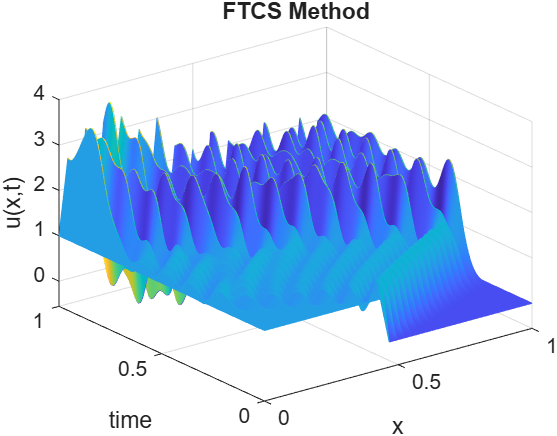
\includegraphics[width=0.7\textwidth]{media2/media/image7.png}
\caption{2D graph of the FTCS method at $c = 2$ with a very small CFL number.}
\label{fig:your_label_name}
\end{figure}

In this case, the small CFL number is illustrated by Figure 5.4. A small CFL number essentially indicates that the time step is much smaller than the spatial step size.

\begin{figure}[H]
\centering
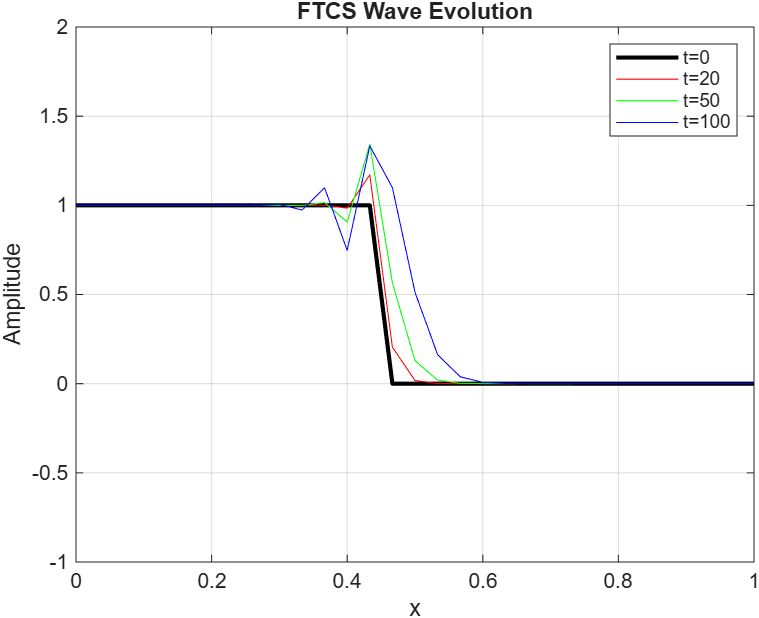
\includegraphics[width=0.7\textwidth]{media2/media/image8.png}
\caption{3D surface plot showing severe oscillations and artificial energy growth for FTCS at $c = 2$.}
\label{fig:your_label_name}
\end{figure}

Bad oscillatory behaviour in the numerical solution can be clearly seen from figure 5.5. Amplitude increases and a very irregular surface develops. The numerical errors are going up pretty crazy as shown on the graph. The FTCS method does not store the original wave energy, but instead increases/artificially amplifies the wave energy.


% ==========================================
\section{Lax Method}
% ==========================================

The Lax Method is used to make FTCS more stable by using the average of nearby points instead of the center point.


The approximation:
\begin{equation*}
\disp_{i}^{n} \rightarrow \frac{1}{2}(\disp_{i + 1}^{n} + \disp_{i - 1}^{n})
\end{equation*}
is used.

If we substitute this into the FTCS scheme, we get:
\begin{equation}
\disp_{i}^{n + 1} = \frac{1}{2}(\disp_{i + 1}^{n} + \disp_{i - 1}^{n}) - \frac{\wavespeed\Delta t}{2\Delta x}(\disp_{i + 1}^{n} - \disp_{i - 1}^{n})
\end{equation}

\subhead{Stability of the Lax Method}

The Lax scheme is conditionally stable. By using von Neumann stability analysis, one obtains the Courant-- Friedrichs--Lewy (CFL) condition:
\begin{equation}
\frac{\wavespeed\Delta t}{\Delta x} \leq 1
\end{equation}

This simply translates to the number's speed needs to be fast enough to follow the true propagation speed.

\subhead{Numerical Diffusion}

Numerical diffusion is an artificial smoothing due to the averaging term. Because of this:
\begin{itemize}
\item the oscillations decreased
\item stability is better
\item wave gets a bit diffused
\end{itemize}

Therefore, LAX method is more stable than the FTCS method but it is simply not as good in keeping the sharp wave fronts.

\subhead{Lax Scheme: Numerical Results and Graphical Interpretation}

The Lax numerical scheme was used to simulate the advection equation. Propagation of the solution is displayed in the following graphs and the stability and diffusive in nature of the method is also indicated:


\noindent \textbf{Lax Method ($c = 1$)}

These graphs represent the numerical solution of the advection equation using the Lax method for $c = 1$.

\begin{figure}[H]
\centering
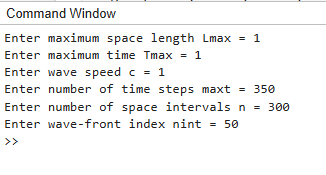
\includegraphics[width=0.45\textwidth]{media2/media/image9.png}
\quad
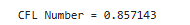
\includegraphics[width=0.35\textwidth]{media2/media/image10.png}
\caption{MATLAB command inputs and the calculated CFL number for the Lax method at $c = 1$.}
\label{fig:your_label_name}
\end{figure}

The surface plot of Figure 5.7 obtained from the Lax method is much smoother than that obtained from the FTCS method. The wave passes consistently through space, with not too bad oscillations.

\begin{figure}[H]
\centering
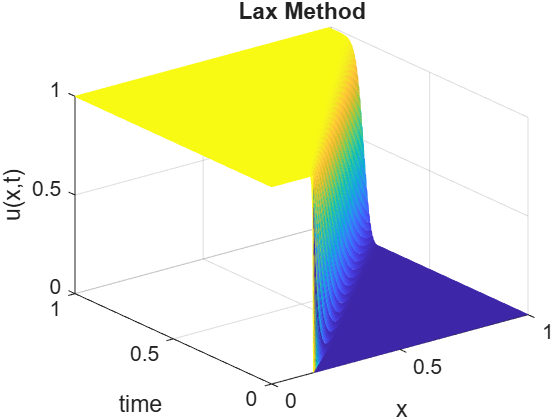
\includegraphics[width=0.45\textwidth]{media2/media/image11.png}
\quad
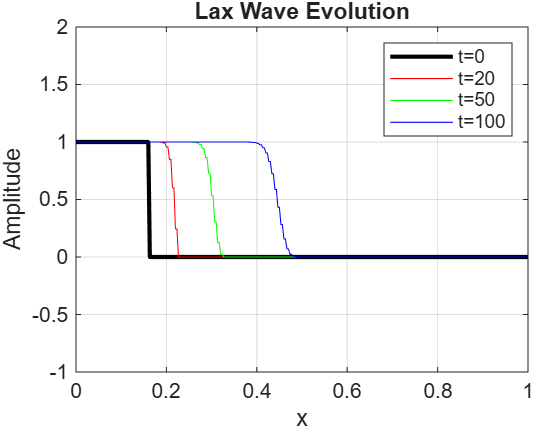
\includegraphics[width=0.45\textwidth]{media2/media/image12.png}
\caption{2D and 3D graphs showing smooth and bounded wave propagation with Lax method at $c = 1$.}
\label{fig:your_label_name}
\end{figure}

It is observed that the wave moves at various time levels as shown in figure 5.7. Does not oscillate strongly and propagates well. Certainly the lax method is more stable than FTCS and the wave front remains in a bounded region.


However, the amplitude of the wave decreases slightly with time. Numerical diffusion is the reason for this.The reason for this is the numerical diffusion which occurs due to the averaging used by the Lax scheme. That method is more stable, but some sharpness and accuracy is lost.

\noindent \textbf{Lax Method ($c = 2$)}

The graphical results presented below have been obtained from the Lax method with a Courant number, $c = 2$.

This plot is for a CFL number larger than one. If its greater than one, it becomes unstable and shows instabilities in the solution.

\begin{figure}[H]
\centering
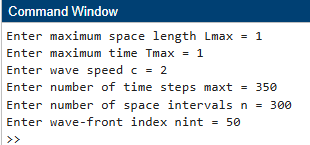
\includegraphics[width=0.45\textwidth]{media2/media/image13.png}
\quad
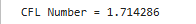
\includegraphics[width=0.35\textwidth]{media2/media/image14.png}
\caption{MATLAB inputs and the calculated CFL number for the Lax method at $c = 2$, showing a CFL violation.}
\label{fig:your_label_name}
\end{figure}

These are big spikes and really large amplitudes in solution figure 5.9. The very large amplitude increase indicates that it's unstable as the CFL criteria was not satisfied. The numerical solution blows up quickly because the time step is too large. This is a graph that illustrates the need for the CFL condition in order to have a stable simulation.

\begin{figure}[H]
\centering
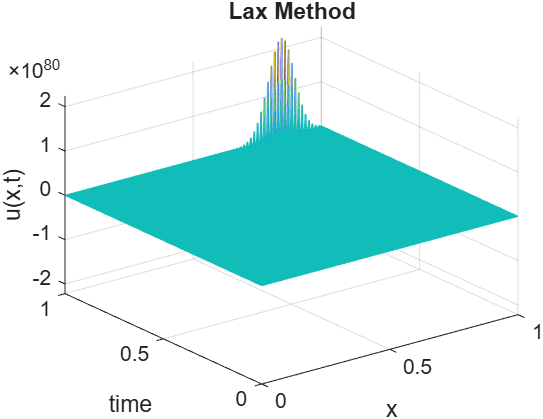
\includegraphics[width=0.7\textwidth]{media2/media/image15.png}
\caption{3D graph showing instability and rapid divergence in the Lax method due to CFL violation at $c = 2$.}
\label{fig:your_label_name}
\end{figure}

As seen in Figure 5.10 the effect of this is that the wave travels more smoothly than FTCS. Although the method remains unchanged, the wave front becomes more and more diffused as the time advances.

This spreading is caused by the numerical diffusion. It eliminates the 'steps' and reduces the 'pointiness' of the wave. The Lax method will provide a stable solution which will also be diffusive.

\begin{figure}[H]
\centering
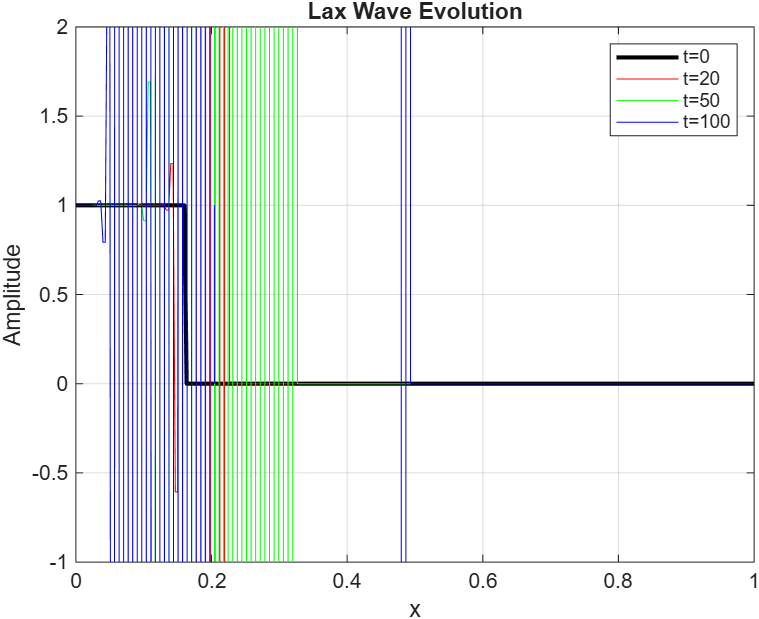
\includegraphics[width=0.8\textwidth]{media2/media/image16.png}
\caption{2D graph showing smoother but spread-out wave propagation for the Lax method at $c = 2$.}
\label{fig:your_label_name}
\end{figure}

% ==========================================
\section{Staggered Leapfrog Method}
% ==========================================

The Leapfrog Method is best for time accuracy and it has less numerical diffusion. It uses centered difference formula in both time and space.

The time derivative is approximated like this:
\begin{equation}
\pd{\disp}{t} \approx \frac{\disp_{i}^{n + 1} - \disp_{i}^{n - 1}}{2\Delta t}
\end{equation}

And the spatial derivative is:
\begin{equation}
\pd{\disp}{x} \approx \frac{\disp_{i + 1}^{n} - \disp_{i - 1}^{n}}{2\Delta x}
\end{equation}

Putting that into the advection equation:
\begin{equation*}
\frac{\disp_{i}^{n + 1} - \disp_{i}^{n - 1}}{2\Delta t} + \wavespeed\frac{\disp_{i + 1}^{n} - \disp_{i - 1}^{n}}{2\Delta x} = 0
\end{equation*}

If you multiply by $2\Delta t$, you get:
\begin{equation}
\disp_{i}^{n + 1} = \disp_{i}^{n - 1} - \frac{\wavespeed\Delta t}{\Delta x}(\disp_{i + 1}^{n} - \disp_{i - 1}^{n})
\end{equation}

\subhead{Properties of the Leapfrog Method}

Advantages:
\begin{itemize}
\item 2nd-order accuracy in time
\item 2nd-order accuracy in space
\item Minimal numerical diffusion
\item Keeps the wave shape better
\end{itemize}

Disadvantages:
\begin{itemize}
\item Might get oscillatory computational modes
\item You need two initial time levels
\item Conditionally stable
\end{itemize}

\subhead{CFL Stability Condition}

The Leapfrog method also needs the CFL condition:
\begin{equation}
\frac{\wavespeed\Delta t}{\Delta x} \leq 1
\end{equation}

If this breaks:
\begin{itemize}
\item the method gets unstable
\item oscillations grow
\item the solution diverges
\end{itemize}

\subhead{Leapfrog Method: Numerical Results and Graphical Interpretation}

We implemented the Leapfrog finite difference method in MATLAB. The graphs below show how accurate and stable the Leapfrog technique is for preserving the wave.

\noindent \textbf{Leapfrog Method ($c = 1$)}

For advection equation, the graphs present the simulation by using the Leapfrog method for $c = 1$.

\begin{figure}[H]
\centering
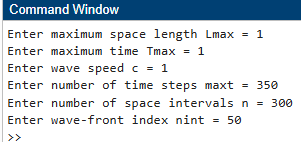
\includegraphics[width=0.45\textwidth]{media2/media/image17.png}
\quad
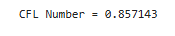
\includegraphics[width=0.35\textwidth]{media2/media/image18.png}
\caption{MATLAB inputs and the calculated CFL number for the Leapfrog method at $c = 1$.}
\label{fig:your_label_name}
\end{figure}

The Leapfrog method is 2nd-order accurate in space and time. Because of that, there's a lot less numerical diffusion compared to the Lax method.

\begin{figure}[H]
\centering
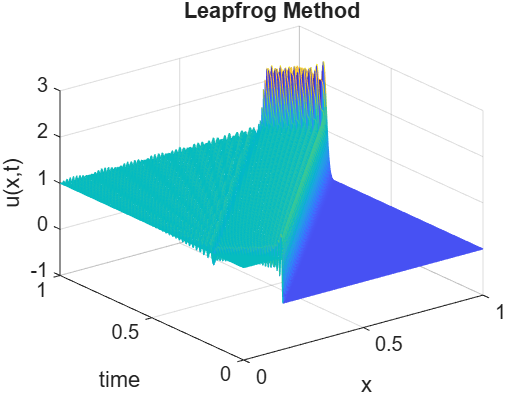
\includegraphics[width=0.45\textwidth]{media2/media/image19.png}
\quad
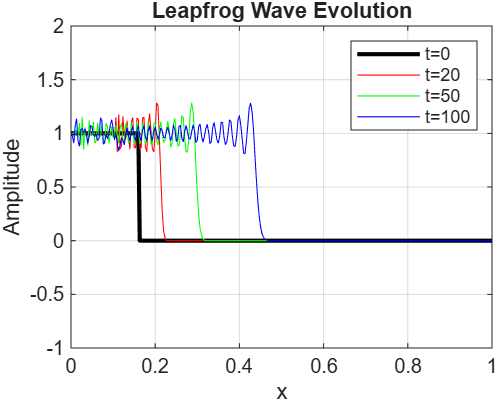
\includegraphics[width=0.45\textwidth]{media2/media/image20.png}
\caption{2D and 3D graphs showing the stability and accuracy of the Leapfrog method at $c = 1$.}
\label{fig:your_label_name}
\end{figure}

Figure 5.12 shows the wave moving at different time levels. The wave keeps its shape way better than the FTCS or Lax methods. Leapfrog is clearly more accurate and stable.

\noindent \textbf{Leapfrog Method ($c = 2$)}

The following graphical results are for the Leapfrog method with a Courant number of $c = 2$.

\begin{figure}[H]
\centering
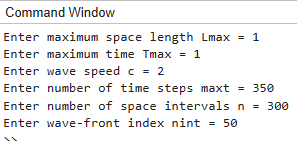
\includegraphics[width=0.45\textwidth]{media2/media/image21.png}
\quad
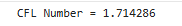
\includegraphics[width=0.35\textwidth]{media2/media/image22.png}
\caption{MATLAB inputs and the calculated CFL number for the Leapfrog method at $c = 2$.}
\label{fig:your_label_name}
\end{figure}

Figure 5.14 shows some big oscillations and weird irregularities in the solution. This instability is because the CFL condition was violated. Numerical errors build up and mess up the wave profile. Even though it's unstable, the solution still keeps more structure than FTCS because the Leapfrog scheme is higher-order accurate.

\begin{figure}
\centering
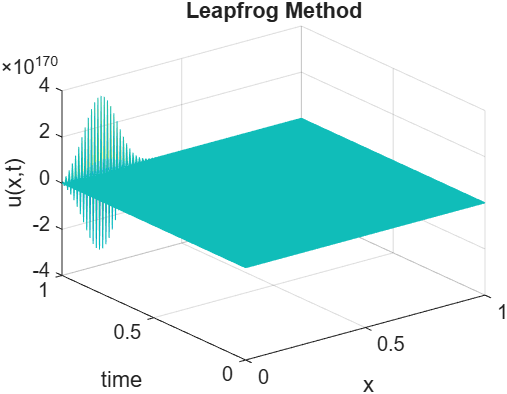
\includegraphics[width=0.7\textwidth]{media2/media/image23.png}
\caption{3D graph showing dispersive oscillations in the Leapfrog method due to a CFL violation at $c = 2$.}
\label{fig:your_label_name}
\end{figure}

\begin{figure}
\centering
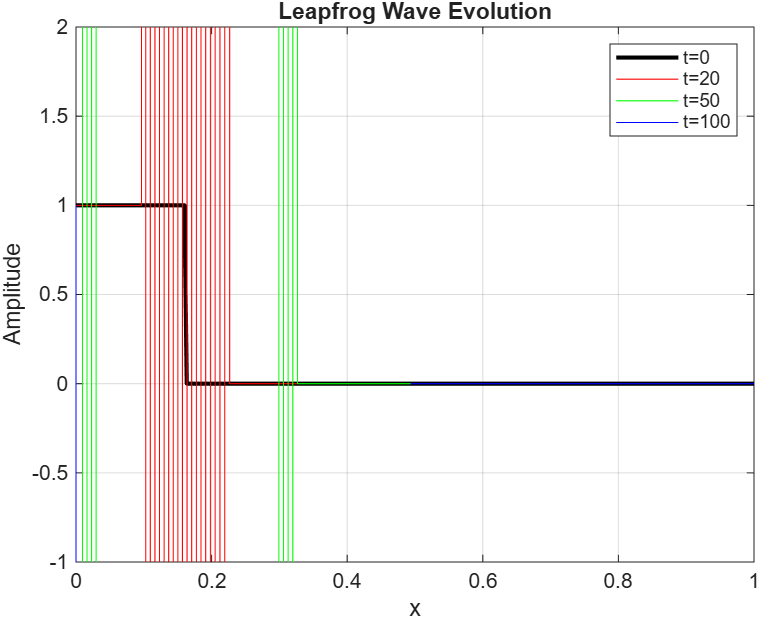
\includegraphics[width=0.7\textwidth]{media2/media/image24.png}
\caption{2D graph showing large dispersive oscillations in the Leapfrog method at $c = 2$, though it still preserves more structure than FTCS.}
\label{fig:your_label_name}
\end{figure}

Figure 5.15 shows that the oscillations are dispersive instead of diffusive. Unlike the Lax method, the Leapfrog scheme doesn't really smooth the solution out.

% ==========================================
\section{Comparison of Numerical Methods}
% ==========================================

\begin{table}[H]
    \centering
    \begin{tabular}{lllc}
        \toprule
        \textbf{Method} & \textbf{Stability}   & \textbf{Accuracy}   & \textbf{Diffusion} \\
        \midrule
        FTCS            & Unstable             & First-order in time & No                 \\
        Lax             & Conditionally Stable & Moderate            & Yes                \\
        Leapfrog        & Conditionally Stable & Second-order        & Very Low           \\
        \bottomrule
    \end{tabular}
    \caption{Comparison of Numerical Methods for advection equation}
\end{table}

\subhead{Comparative Analysis of FTCS, Lax, and Leapfrog Methods By Example}

The following graphs present a comparative analysis of the FTCS, Lax, and Leapfrog methods using the same initial conditions and identical numerical parameters. The results provide a clear comparison of the stability, convergence, and accuracy of the three numerical schemes for solving the advection equation.

For the first example, let's look at the first-order wave equation:
\begin{equation}
\pd{\disp}{t} = -a \pd{\disp}{x} \qquad a > 0 \tag{6-24}
\end{equation}
where $a$ is the speed of sound, which we set to $250 \text{ m/s}$. We'll assume at time $t = 0$, there's a half-sinusoidal disturbance. The initial condition is:
\begin{equation}
    \left.
    \begin{aligned}
        \disp(x,0) & = 0                                                                                   &  & 0 \le x \le 50    \\
        \disp(x,0) & = 100 \left\{ \sin \left[ \pi \left( \frac{x - 50}{60} \right) \right] \right\} \quad &  & 50 \le x \le 110  \\
        \disp(x,0) & = 0                                                                                   &  & 110 \le x \le 400
    \end{aligned}
    \right\} \tag{6-25}
\end{equation}

\begin{figure}[H]
    \centering
    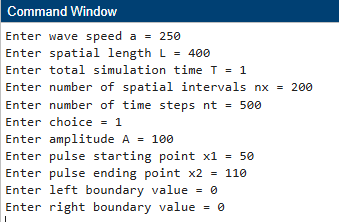
\includegraphics[width=0.5\textwidth]{media2/media/image25.png}
    \caption{Input commands establishing identical initial conditions and numerical parameters for comparing the FTCS, Lax, and Leapfrog methods.}
    \label{fig:your_label_name}
\end{figure}


\subsection{FTCS Method}

\begin{figure}[H]
\centering
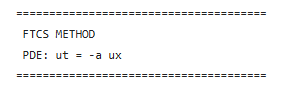
\includegraphics[width=0.45\textwidth]{media2/media/image26.png}
\quad
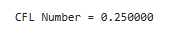
\includegraphics[width=0.35\textwidth]{media2/media/image27.png}
\caption{Output representing the initial wave condition before propagation for the FTCS simulation.}
\label{fig:your_label_name}
\end{figure}

Figure 5.18 shows the starting condition before the wave propagates. The FTCS method starts amplifying errors pretty early on. The wave front loses its smoothness and stability.

\begin{figure}[H]
\centering
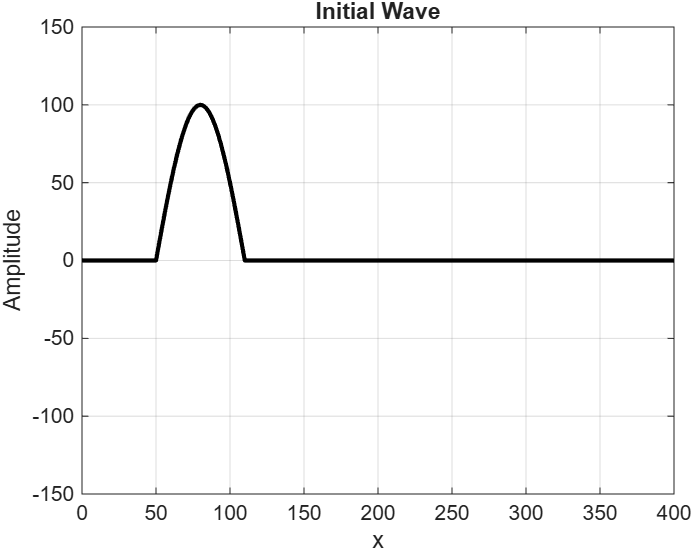
\includegraphics[width=0.7\textwidth]{media2/media/image28.png}
\caption{2D graph of the early FTCS simulation where errors start amplifying.}
\label{fig:your_label_name}
\end{figure}

In Figure 5.19, the FTCS method is already starting to amplify the errors. The wave front isn't smooth anymore.

\begin{figure}[H]
\centering
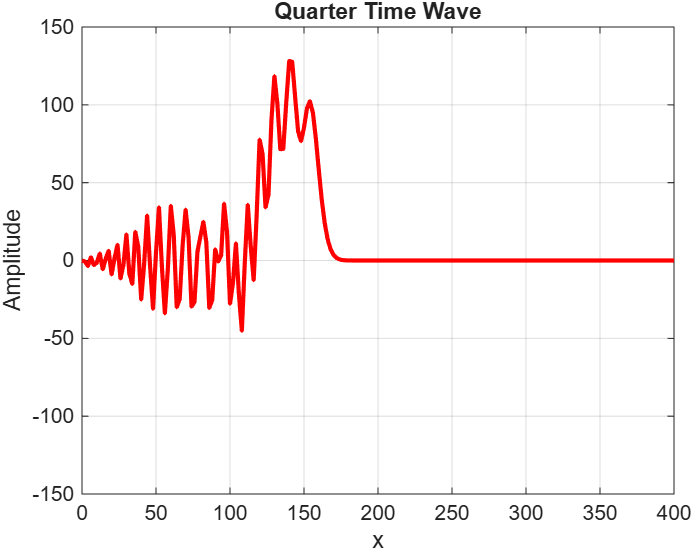
\includegraphics[width=0.7\textwidth]{media2/media/image29.png}
\caption{2D graph of FTCS method at half time, representing distorted wave and strong oscillations.}
\label{fig:your_label_name}
\end{figure}
The oscillations are getting way stronger by the halfway point in Figure 5.20. The profile is pretty distorted and the solution is not reliable anymore.

\begin{figure}[H]
\centering
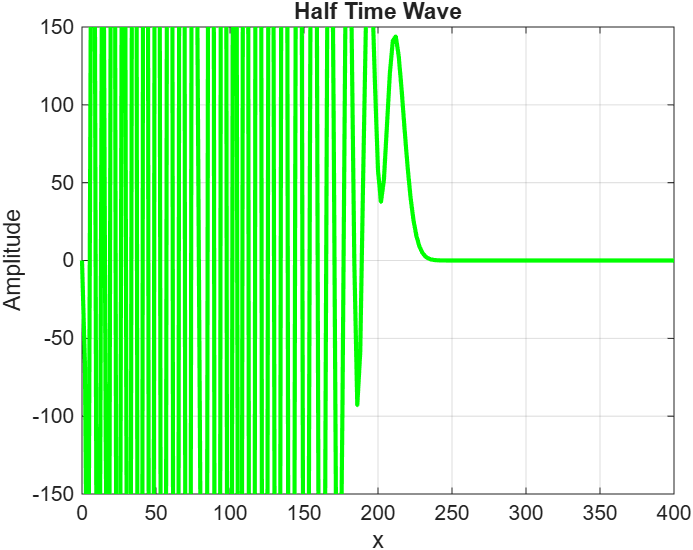
\includegraphics[width=0.8\textwidth]{media2/media/image30.png}
\caption{2D graph comparing initial, quarter, half, and final wave for FTCS.}
\label{fig:your_label_name}
\end{figure}

It compares all the profiles from initial to the end in Figure 5.21. The FTCS method really does not give a good result for long-term wave propagation.

\begin{figure}[H]
\centering
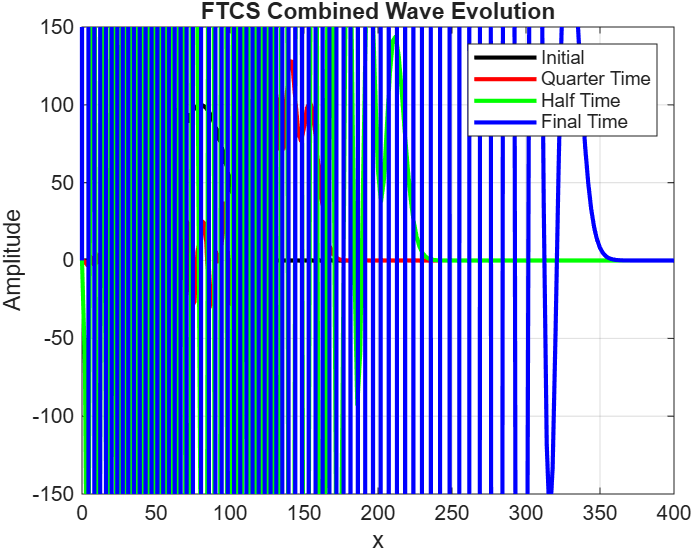
\includegraphics[width=0.8\textwidth]{media2/media/image31.png}

\caption{2D graph showing the uncontrollable amplitude growth for the unstable FTCS method.}
\label{fig:your_label_name}
\end{figure}

\noindent \textbf{Conclusions}

The amplitude just keeps growing and you can't even see the original pulse shape anymore. The FTCS method doesn't work for long-term simulations.

\subsection{Lax Method}

\begin{figure}[H]
\centering
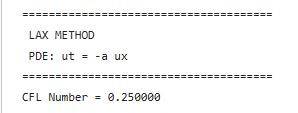
\includegraphics[width=0.45\textwidth]{media2/media/image32.png}
\caption{Output parameters for the Lax method analysis.}
\label{fig:your_label_name}
\end{figure}

\begin{figure}[H]
\centering
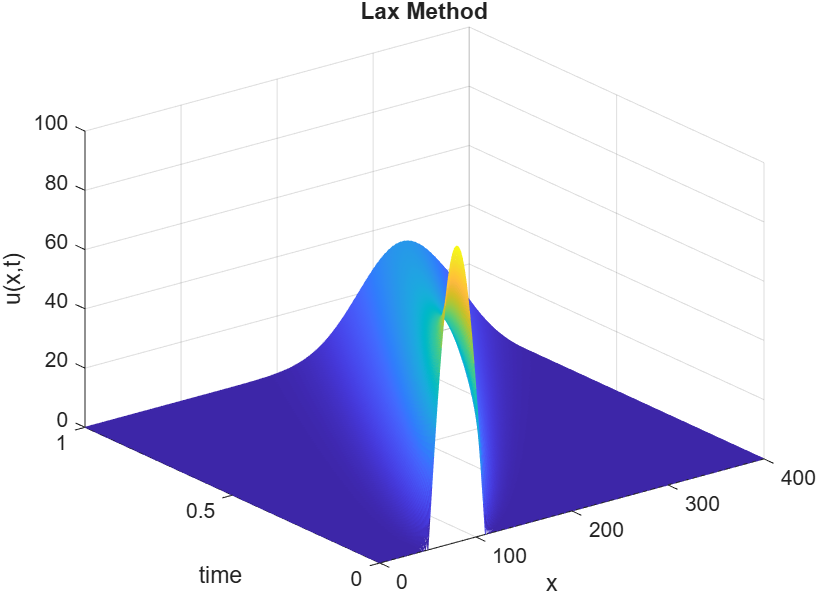
\includegraphics[width=0.8\textwidth]{media2/media/image33.png}
\caption{3D surface plot of the Lax method showing smooth, stable wave propagation.}
\label{fig:your_label_name}
\end{figure}

Figure 5.23 from the Lax method shows smooth and stable wave propagation.

\section{Overall Discussion}

The graphical analysis shows some major differences between FTCS, Lax, and Leapfrog methods.

\subsection*{FTCS Method}
\begin{itemize}
\item It's unstable for the advection equation.
\item It makes growing oscillations.
\item It fails to converge.
\item The solution becomes non-physical.
\end{itemize}

\subsection*{Lax Method}
\begin{itemize}
\item Stable if you follow the CFL condition.
\item Suppresses oscillations.
\item Adds numerical diffusion.
\item The solutions are smoother but not as sharp.
\end{itemize}

\subsection*{Leapfrog Method}
\begin{itemize}
\item It's a higher-order accurate scheme.
\item It keeps the wave shape pretty well.
\item Very little numerical diffusion.
\item Small dispersive oscillations might appear.
\item Overall, it gives the best numerical performance.
\end{itemize}
%%%%%%%%%%%%%%%%%%%%%%%%%%%%%%%%%%%%%%%%%%%%%%%%%%%%%%%%%%%%
% ==========================================
\section{Conclusion}
% ==========================================

Looking at all three methods:

\begin{enumerate}
\item FTCS is unstable, so it's not good for long simulations.
\item Lax is stable, but it's diffusive.
\item Leapfrog is stable, accurate, and preserves the wave structure the best.
\end{enumerate}

As a result, the Leapfrog approach is most appropriate for solving advection/wave equation in this study.

% ==========================================
\section{Sources of Errors in Numerical Methods}
% ==========================================

Numerical methods have errors because we are just approximating the derivatives. The main errors are:
\begin{itemize}
\item truncation error
\item round-off error
\item discretization error
\end{itemize}

\subhead{Consistency}

A method is consistent if the approximation gets closer to the original PDE as:
\begin{equation*}
\Delta x \rightarrow 0 \quad \text{and} \quad \Delta t \rightarrow 0
\end{equation*}

\subhead{Stability}

The method is said to be stable if the errors don't grow uncontrollably while you're calculating. A stable method keeps errors bounded as time goes on.

\subhead{Convergence}

A method converges if the numerical solution gets closer to the real analytical solution as:
\begin{equation*}
\Delta x \rightarrow 0 \quad \text{and} \quad \Delta t \rightarrow 0
\end{equation*}

\subhead{Relationship between Consistency, Convergence and Stability}

According to the Lax Equivalence Theorem:
\begin{equation*}
\text{Consistency} + \text{Stability} = \text{Convergence}
\end{equation*}

This indicates that if a scheme is stable and consistent , it will converge to the correct solution.

% ==========================================
\chapter{Numerical Solutions for Heat or Diffusion Equation}
% ==========================================

\section{Introduction}

The heat equation, often known as the diffusion equation, is a fundamental partial differential equation in applied mathematics, physics, and engineering. It shows how heat is distributed and flows through a material over time. The equation is commonly used in thermal engineering, fluid mechanics, material science, and diffusion processes.

The 1-dimensional heat equation is given by:
\begin{equation}
    \pd{\disp}{t} = D\pdd{\disp}{x}
\end{equation}

Where:
\begin{itemize}
    \item $\disp(x,t)$ represents the wave amplitude or transported quantity.
    \item $c$ is the propagation velocity.
    \item $x$ is the spatial coordinate.
    \item $D$ is the diffusion coefficient or thermal conductivity.
\end{itemize}

The L.H.S of the equation shows the rate of change of temperature with respect to time, while the right-hand side presents the spatial diffusion of heat.

In this chapter, numerical techniques are applied to find the solution of the 1-dimensional heat equation. First, the FTCS explicit finite difference method is derived and implemented. Then, Von Neumann stability analysis is performed to observe the stability behavior of the explicit scheme. Finally, the Crank--Nicolson implicit method is derived, analyzed, and implemented.

% ==========================================
\section{Discretization}
% ==========================================

To numerically solve the heat equation, the continuous space and time domains are discretized into a finite grid.

The spatial domain is divided as:
\begin{equation*}
    x_{i} = i\Delta x
\end{equation*}

where:
\begin{itemize}
    \item $\Delta x$ is the spatial step size,
    \item $i = 0, 1, \dots, n$
\end{itemize}

Similarly, the time domain is discretized as:
\begin{equation*}
    t_{j} = j\Delta t
\end{equation*}

where:
\begin{itemize}
    \item $\Delta t$ is the time step size,
    \item $j = 0, 1, 2, \dots$
\end{itemize}

The numerical approximation of the temperature at the mesh point $(x_{i}, t_{j})$ is represented by:
\begin{equation*}
    \disp_{i}^{j}
\end{equation*}

The finite difference grid consists of neighboring points in both space and time. These neighboring points are used to approximate the derivatives appearing in the PDE.

% ==========================================
\section{FTCS Explicit Method for the Heat Equation}
% ==========================================

The FTCS (Forward Time Centered Space) method is an explicit finite difference scheme used to solve the heat equation.

The method uses:
\begin{itemize}
    \item Forward difference approximation in time,
    \item Central difference approximation in space.
\end{itemize}

\subsection{Forward Difference Approximation in Time}

The 1st-order derivative of time is approximated by using the forward difference formula:
\begin{equation}
    \pd{\disp}{t} \approx \frac{\disp_{i}^{j + 1} - \disp_{i}^{j}}{\Delta t}
\end{equation}
This approximation uses the current time level ($j$) and the next time level ($j + 1$).

\subsection{Central Difference Approximation in Space}

The 2nd-order spatial derivative is calculated by using the central difference formula:
\begin{equation}
    \pdd{\disp}{x} \approx \frac{\disp_{i + 1}^{j} - 2\disp_{i}^{j} + \disp_{i - 1}^{j}}{(\Delta x)^{2}}
\end{equation}
This approximation uses the neighboring spatial points around the central node.

\subsection{Derivation of the FTCS Scheme}

Starting with heat equation:
\begin{equation*}
    \pd{\disp}{t} = D\pdd{\disp}{x}
\end{equation*}

Substituting the finite difference approximations gives:
\begin{equation*}
    \frac{\disp_{i}^{j + 1} - \disp_{i}^{j}}{\Delta t} = D\frac{\disp_{i + 1}^{j} - 2\disp_{i}^{j} + \disp_{i - 1}^{j}}{(\Delta x)^{2}}
\end{equation*}

Multiplying both sides by $\Delta t$:
\begin{equation*}
    \disp_{i}^{j + 1} - \disp_{i}^{j} = \frac{D\Delta t}{(\Delta x)^{2}}\left(\disp_{i + 1}^{j} - 2\disp_{i}^{j} + \disp_{i - 1}^{j}\right)
\end{equation*}

The stability parameter is defined as:
\begin{equation*}
    \alpha = \frac{D\Delta t}{(\Delta x)^{2}}
\end{equation*}

Then the equation becomes:
\begin{equation*}
    \disp_{i}^{j + 1} - \disp_{i}^{j} = \alpha(\disp_{i + 1}^{j} - 2\disp_{i}^{j} + \disp_{i - 1}^{j})
\end{equation*}

Expanding the right-hand side:
\begin{equation*}
    \disp_{i}^{j + 1} = \disp_{i}^{j} + \alpha \disp_{i + 1}^{j} - 2\alpha \disp_{i}^{j} + \alpha \disp_{i - 1}^{j}
\end{equation*}

Grouping terms:
\begin{equation}
    \disp_{i}^{j + 1} = \alpha \disp_{i + 1}^{j} + (1 - 2\alpha)\disp_{i}^{j} + \alpha \disp_{i - 1}^{j}
\end{equation}

This is the FTCS explicit finite difference scheme for the one-dimensional heat equation.

\subsection{Characteristics of the FTCS Method}

FTCS method is known as explicit due to the future value $\disp_{i}^{j + 1}$ is computed directly from the known values at the previous time level.

Advantages of the FTCS method include:
\begin{itemize}
    \item Simple implementation,
    \item Direct computation of future values,
    \item Low computational complexity.
\end{itemize}

However, the scheme is conditionally stable and needs a restriction on the time step size.

% ==========================================
\section{Von Neumann Stability Analysis of the FTCS Scheme}
% ==========================================

The stability of the FTCS method is investigated using the Von Neumann stability analysis. The analysis aims to detect whether numerical mistakes increase or decrease as the calculation progresses over time.

\subsection{Fourier Error Assumption}

\begin{equation*}
    \disp_{i}^{n} = \xi^{n}e^{ikx_{i}}
\end{equation*}

where:
\begin{itemize}
    \item $\xi$ is the amplification factor,
    \item $k$ is the wave number,
    \item $x_{i} = i\Delta x$
\end{itemize}

The stability of the numerical scheme depends on the magnitude of the amplification factor. The method is stable if:
\begin{equation}
    |\xi| \leq 1
\end{equation}

\subsection{Substitution into the FTCS Scheme}

The FTCS scheme is:
\begin{equation*}
    \disp_{i}^{n + 1} = \disp_{i}^{n} + \alpha(\disp_{i + 1}^{n} - 2\disp_{i}^{n} + \disp_{i - 1}^{n})
\end{equation*}

Substitute:
\begin{equation*}
    \disp_{i}^{n} = \xi^{n}e^{ikx_{i}}
\end{equation*}

Then:
\begin{equation*}
    \disp_{i + 1}^{n} = \xi^{n}e^{ik(x_{i} + \Delta x)} = \xi^{n}e^{ikx_{i}}e^{ik\Delta x}
\end{equation*}
and:
\begin{equation*}
    \disp_{i - 1}^{n} = \xi^{n}e^{ik(x_{i} - \Delta x)} = \xi^{n}e^{ikx_{i}}e^{- ik\Delta x}
\end{equation*}

Substituting into the FTCS equation:
\begin{equation*}
    \xi^{n + 1}e^{ikx_{i}} = \xi^{n}e^{ikx_{i}} \left[ 1 + \alpha\left( e^{ik\Delta x} - 2 + e^{- ik\Delta x} \right) \right]
\end{equation*}

Dividing both sides by $\xi^{n}e^{ikx_{i}}$:
\begin{equation*}
    \xi = 1 + \alpha\left( e^{ik\Delta x} - 2 + e^{- ik\Delta x} \right)
\end{equation*}

Using Euler's identity:
\begin{equation*}
    e^{i\theta} + e^{- i\theta} = 2\cos\theta
\end{equation*}
Take $\theta = k\Delta x$. Therefore:
\begin{equation*}
    e^{ik\Delta x} + e^{- ik\Delta x} = 2\cos(k\Delta x)
\end{equation*}

Substitute:
\begin{equation*}
    \xi = 1 + \alpha(2\cos(k\Delta x) - 2)
\end{equation*}

Factor 2:
\begin{equation}
    \xi = 1 + 2\alpha(\cos(k\Delta x) - 1)
\end{equation}

Using the trigonometric identity:
\begin{equation*}
    \cos\theta - 1 = - 2\sin^{2}\left( \frac{\theta}{2} \right)
\end{equation*}

Take $\theta = k\Delta x$. Then:
\begin{equation*}
    \cos(k\Delta x) - 1 = - 2\sin^{2}\left( \frac{k\Delta x}{2} \right)
\end{equation*}

Substitute:
\begin{equation*}
    \xi = 1 + 2\alpha\left[ - 2\sin^{2}\left( \frac{k\Delta x}{2} \right) \right]
\end{equation*}

Simplify:
\begin{equation}
    \xi = 1 - 4\alpha\sin^{2}\left( \frac{k\Delta x}{2} \right)
\end{equation}

Here:
\begin{equation*}
    \alpha = \frac{D\Delta t}{(\Delta x)^{2}}
\end{equation*}

Finally:
\begin{equation}
    \xi = 1 - 4\frac{D\Delta t}{(\Delta x)^{2}}\sin^{2}\left( \frac{k\Delta x}{2} \right)
\end{equation}

\subsection{Stability Condition}

For stability:
\begin{equation*}
    |\xi| \leq 1
\end{equation*}

Since:
\begin{equation*}
    0 \leq \sin^{2}\left( \frac{k\Delta x}{2} \right) \leq 1
\end{equation*}

The most restrictive case occurs when:
\begin{equation*}
    \sin^{2}\left( \frac{k\Delta x}{2} \right) = 1
\end{equation*}

Then:
\begin{equation*}
    \xi_{\min} = 1 - 4\alpha
\end{equation*}

For stability:
\begin{equation*}
    - 1 \leq 1 - 4\alpha \leq 1
\end{equation*}
Focusing on the lower bound:
\begin{equation*}
    - 1 \leq 1 - 4\alpha
\end{equation*}
Subtract 1:
\begin{equation*}
    - 2 \leq - 4\alpha
\end{equation*}
Multiply by $- 1$ (flips inequality):
\begin{equation*}
    2 \geq 4\alpha
\end{equation*}
Divide by 4:
\begin{equation*}
    \alpha \leq \frac{1}{2}
\end{equation*}

Substitute back:
\begin{equation}
    \frac{D\Delta t}{(\Delta x)^{2}} \leq \frac{1}{2}
\end{equation}
Or equivalently:
\begin{equation}
    \frac{2D\Delta t}{(\Delta x)^{2}} \leq 1
\end{equation}

This is the Von Neumann stability condition for the FTCS explicit method.

\subsection{Interpretation of Stability}

If the stability condition is met:
\begin{itemize}
\item The numerical solution stays smooth,
\item Errors decay over time,
\item The solution behaves physically.
\end{itemize}

If the stability condition is violated:
\begin{itemize}
\item Oscillations start appearing,
\item Numerical errors grow really fast,
\item The solution becomes unstable and starts diverging.
\end{itemize}

So, the explicit FTCS method requires a pretty small time step for the computation to remain stable.

\begin{figure}[H]
\centering

\includegraphics[width=0.45\textwidth]{media_missing/media/image1.png}
\quad

\includegraphics[width=0.3\textwidth]{media_missing/media/image2.png}
\caption{FTCS method stability profiles}
\end{figure}

The fig 6.2 graph shows that the FTCS explicit method successfully approximates the heat diffusion process when the stability condition is satisfied.

\begin{figure}[H]
\centering

\includegraphics[width=0.8\textwidth]{media_missing/media/image3.png}
\caption{FTCS explicit method numerical solution representation}
\end{figure}
The 3D surface plot in fig 6.3 verifies that the Explicit FTCS method provides a stable and accurate enough numerical approximation of the heat diffusion equation when the stability criteria is properly met.
\begin{figure}[H]
\centering

\includegraphics[width=0.8\textwidth]{media_missing/media/image4.png}
\caption{Detailed profile of FTCS error amplification}
\end{figure}

Figure 6.4 illustrates the initial development of numerical instability in the Forward-Time Central-Space explicit scheme for 1-dimensional heat equation when the stability criteria is violated.

\begin{figure}[H]
\centering

\includegraphics[width=0.45\textwidth]{media_missing/media/image5.png}
\quad

\includegraphics[width=0.35\textwidth]{media_missing/media/image6.png}
\caption{FTCS instability behavior}
\end{figure}

In fig 6.5 the temperature profile exhibits large oscillations with really high positive and negative values. Instead of showing smooth heat diffusion, the solution fluctuates uncontrollably and deviates from the expected physical behavior.This indicates that numerical errors are being amplified at each time step, causing the solution to diverge rather than converge. The oscillatory pattern confirms the instability of the FTCS scheme when the stability condition is violated.This continuous error growth shows the failure of the conditionally stable FTCS explicit scheme when the step size limits are violated, resulting in a divergent, non-physical wave profile that is completely detached from the true solution.

\begin{figure}[H]
\centering

\includegraphics[width=0.8\textwidth]{media_missing/media/image7.png}
\caption{Long-term divergence in FTCS explicitly computed solution}
\end{figure}

The fig 6.6 3D surface plot shows a rapid growth of the solution magnitude, reaching extremely large values. Such behavior is physically impossible for a heat diffusion problem and clearly indicates numerical blow-up.The sharp spikes and irregular surface demonstrate that the numerical errors dominate the solution as time progresses. Consequently, the computed temperature distribution becomes meaningless and cannot really represent the actual diffusion process.

\begin{figure}[H]
\centering

\includegraphics[width=0.8\textwidth]{media_missing/media/image8.png}
\caption{Final state of numerical errors causing instability}
\end{figure}

% ==========================================
\section{Crank--Nicolson Method}
% ==========================================

The Crank--Nicolson method is an implicit finite difference method that mixes the stability of implicit schemes with second-order accuracy in both time and space.

The method is obtained by averaging the explicit FTCS scheme and the implicit BTCS (Backward Time Centered Space) scheme.
\subsection{BTCS Implicit Scheme}

The BTCS discretization of the heat equation is:
\begin{equation}
    \frac{\disp_{i}^{n + 1} - \disp_{i}^{n}}{\Delta t} = D\frac{\disp_{i + 1}^{n + 1} - 2\disp_{i}^{n + 1} + \disp_{i - 1}^{n + 1}}{(\Delta x)^{2}}
\end{equation}

In this method, all spatial terms are evaluated at the future time level $(n + 1)$.

\subsection{Derivation of the Crank--Nicolson Scheme}

The Crank--Nicolson method averages the explicit FTCS and implicit BTCS schemes.
\begin{equation*}
    CN = \frac{1}{2}(\text{Explicit} + \text{Implicit})
\end{equation*}

Thus:
\begin{equation}
    \frac{\disp_{i}^{n + 1} - \disp_{i}^{n}}{\Delta t} = \frac{D}{2}\left[ \frac{\disp_{i + 1}^{n} - 2\disp_{i}^{n} + \disp_{i - 1}^{n}}{(\Delta x)^{2}} + \frac{\disp_{i + 1}^{n + 1} - 2\disp_{i}^{n + 1} + \disp_{i - 1}^{n + 1}}{(\Delta x)^{2}} \right]
\end{equation}

Taking a common denominator:
\begin{equation*}
    \frac{\disp_{i}^{n + 1} - \disp_{i}^{n}}{\Delta t} = \frac{D}{2(\Delta x)^{2}}\left[ \disp_{i + 1}^{n} - 2\disp_{i}^{n} + \disp_{i - 1}^{n} + \disp_{i + 1}^{n + 1} - 2\disp_{i}^{n + 1} + \disp_{i - 1}^{n + 1} \right]
\end{equation*}

Multiplying by $\Delta t$:
\begin{equation*}
    \disp_{i}^{n + 1} - \disp_{i}^{n} = \frac{D(\Delta t)}{2(\Delta x)^{2}}\left[ \disp_{i + 1}^{n} - 2\disp_{i}^{n} + \disp_{i - 1}^{n} + \disp_{i + 1}^{n + 1} - 2\disp_{i}^{n + 1} + \disp_{i - 1}^{n + 1} \right]
\end{equation*}

Define:
\begin{equation*}
    \alpha = \frac{D\Delta t}{(\Delta x)^{2}}
\end{equation*}

Then:
\begin{equation*}
    \frac{D(\Delta t)}{2(\Delta x)^{2}} = \frac{\alpha}{2}
\end{equation*}

So the equation becomes:
\begin{equation*}
    \disp_{i}^{n + 1} - \disp_{i}^{n} = \frac{\alpha}{2}\left[ \disp_{i + 1}^{n} - 2\disp_{i}^{n} + \disp_{i - 1}^{n} + \disp_{i + 1}^{n + 1} - 2\disp_{i}^{n + 1} + \disp_{i - 1}^{n + 1} \right]
\end{equation*}

Expanding the brackets:
\begin{equation*}
    \disp_{i}^{n + 1} - \disp_{i}^{n} = \frac{\alpha}{2}\disp_{i + 1}^{n} - \alpha \disp_{i}^{n} + \frac{\alpha}{2}\disp_{i - 1}^{n} + \frac{\alpha}{2}\disp_{i + 1}^{n + 1} - \alpha \disp_{i}^{n + 1} + \frac{\alpha}{2}\disp_{i - 1}^{n + 1}
\end{equation*}

Move all future terms to the left-hand side:
\begin{equation*}
    \disp_{i}^{n + 1} + \alpha \disp_{i}^{n + 1} - \frac{\alpha}{2}\disp_{i + 1}^{n + 1} - \frac{\alpha}{2}\disp_{i - 1}^{n + 1} = \disp_{i}^{n} + \frac{\alpha}{2}\disp_{i + 1}^{n} - \alpha \disp_{i}^{n} + \frac{\alpha}{2}\disp_{i - 1}^{n}
\end{equation*}

Grouping terms:
\begin{equation*}
    - \frac{\alpha}{2}\disp_{i - 1}^{n + 1} + (1 + \alpha)\disp_{i}^{n + 1} - \frac{\alpha}{2}\disp_{i + 1}^{n + 1} = \frac{\alpha}{2}\disp_{i - 1}^{n} + (1 - \alpha)\disp_{i}^{n} + \frac{\alpha}{2}\disp_{i + 1}^{n}
\end{equation*}

This is the Crank--Nicolson finite difference equation. After algebra (multiplying by 2):
\begin{equation}
    - \alpha \disp_{i - 1}^{n + 1} + (2 + 2\alpha)\disp_{i}^{n + 1} - \alpha \disp_{i + 1}^{n + 1} = \alpha \disp_{i - 1}^{n} + (2 - 2\alpha)\disp_{i}^{n} + \alpha \disp_{i + 1}^{n}
\end{equation}

This is the main CN algebraic equation.

% ==========================================
\section{Matrix Formulation of the Crank--Nicolson Method}
% ==========================================

Compared to
Compared to the FTCS explicit scheme, the Crank--Nicolson scheme contains unknown future values at neighboring nodes. Therefore, all equations are coupled together and must be solved simultaneously.

Building the matrix:
\begin{equation*}
    M_{l}U^{n + 1} = M_{r}U^{n} + r^{n}
\end{equation*}

Unknown vector:
\begin{equation*}
    U^{n + 1} = \begin{bmatrix}
        \disp_{1}^{n + 1} \\
        \disp_{2}^{n + 1} \\
        \disp_{3}^{n + 1}
    \end{bmatrix}
\end{equation*}

Assume a small grid where $n = 4$. Unknown points:
\begin{equation*}
    \disp_{1}^{n + 1}, \disp_{2}^{n + 1}, \disp_{3}^{n + 1}, \disp_{4}^{n + 1}
\end{equation*}

Boundary values are known:
\begin{equation*}
    \disp_{0} = 0, \quad \disp_{5} = 0
\end{equation*}

\subhead{For $\mathbf{i = 1:}$}
CN formula:
\begin{equation*}
    - \alpha \disp_{0}^{n + 1} + (2 + 2\alpha)\disp_{1}^{n + 1} - \alpha \disp_{2}^{n + 1} = RHS
\end{equation*}
Since $\disp_{0}^{n + 1} = 0$, then:
\begin{equation*}
    (2 + 2\alpha)\disp_{1}^{n + 1} - \alpha \disp_{2}^{n + 1} = RHS
\end{equation*}

\begin{table}[H]
    \centering
    \begin{tabular}{ll}
        \toprule
        \textbf{Unknown}    & \textbf{Coefficient} \\
        \midrule
        $\disp_{1}^{n + 1}$ & $2 + 2\alpha$        \\
        $\disp_{2}^{n + 1}$ & $-\alpha$            \\
        $\disp_{3}^{n + 1}$ & $0$                  \\
        $\disp_{4}^{n + 1}$ & $0$                  \\
        \bottomrule
    \end{tabular}
    \caption{Coefficients for $i=1$}
\end{table}

So the first matrix row is: $\begin{bmatrix} 2 + 2\alpha & -\alpha & 0 & 0 \end{bmatrix}$

\subhead{For $\mathbf{i = 2:}$}
Now:
\begin{equation*}
    - \alpha \disp_{1}^{n + 1} + (2 + 2\alpha)\disp_{2}^{n + 1} - \alpha \disp_{3}^{n + 1} = RHS
\end{equation*}

\begin{table}[H]
    \centering
    \begin{tabular}{ll}
        \toprule
        \textbf{Unknown}    & \textbf{Coefficient} \\
        \midrule
        $\disp_{1}^{n + 1}$ & $-\alpha$            \\
        $\disp_{2}^{n + 1}$ & $2 + 2\alpha$        \\
        $\disp_{3}^{n + 1}$ & $-\alpha$            \\
        $\disp_{4}^{n + 1}$ & $0$                  \\
        \bottomrule
    \end{tabular}
    \caption{Coefficients for $i=2$}
\end{table}

So the row becomes: $\begin{bmatrix} -\alpha & 2 + 2\alpha & -\alpha & 0 \end{bmatrix}$

\subhead{For $\mathbf{i = 3:}$}
So:
\begin{equation*}
    - \alpha \disp_{2}^{n + 1} + (2 + 2\alpha)\disp_{3}^{n + 1} - \alpha \disp_{4}^{n + 1} = RHS
\end{equation*}

\begin{table}[H]
    \centering
    \begin{tabular}{ll}
        \toprule
        \textbf{Unknown}    & \textbf{Coefficient} \\
        \midrule
        $\disp_{1}^{n + 1}$ & $0$                  \\
        $\disp_{2}^{n + 1}$ & $-\alpha$            \\
        $\disp_{3}^{n + 1}$ & $2 + 2\alpha$        \\
        $\disp_{4}^{n + 1}$ & $-\alpha$            \\
        \bottomrule
    \end{tabular}
    \caption{Coefficients for $i=3$}
\end{table}

Row becomes: $\begin{bmatrix} 0 & -\alpha & 2 + 2\alpha & -\alpha \end{bmatrix}$

\subhead{For $\mathbf{i = 4:}$}
\begin{equation*}
    - \alpha \disp_{3}^{n + 1} + (2 + 2\alpha)\disp_{4}^{n + 1} = RHS
\end{equation*}

\begin{table}[H]
    \centering
    \begin{tabular}{ll}
        \toprule
        \textbf{Unknown}    & \textbf{Coefficient} \\
        \midrule
        $\disp_{1}^{n + 1}$ & $0$                  \\
        $\disp_{2}^{n + 1}$ & $0$                  \\
        $\disp_{3}^{n + 1}$ & $-\alpha$            \\
        $\disp_{4}^{n + 1}$ & $2 + 2\alpha$        \\
        \bottomrule
    \end{tabular}
    \caption{Coefficients for $i=4$}
\end{table}

So row becomes: $\begin{bmatrix} 0 & 0 & -\alpha & 2 + 2\alpha \end{bmatrix}$

Left matrix $M_{l}$:
\begin{equation*}
    M_{l} = \begin{bmatrix}
        2 + 2\alpha & -\alpha     & 0           & 0           \\
        -\alpha     & 2 + 2\alpha & -\alpha     & 0           \\
        0           & -\alpha     & 2 + 2\alpha & -\alpha     \\
        0           & 0           & -\alpha     & 2 + 2\alpha
    \end{bmatrix}
\end{equation*}

Right matrix components ($M_{r}$) are constructed from:
\begin{equation*}
    \alpha \disp_{i - 1}^{n} + (2 - 2\alpha)\disp_{i}^{n} + \alpha \disp_{i + 1}^{n}
\end{equation*}

These equations can be written in the form of matrix as:
\begin{equation}
    A U^{n + 1} = B U^{n}
\end{equation}

Where $A$ (using the standard $1+\alpha$ normalization) is:
\begin{equation*}
    A = \begin{bmatrix}
        (1 + \alpha)      & -\frac{\alpha}{2} & 0                 & 0                 \\
        -\frac{\alpha}{2} & (1 + \alpha)      & -\frac{\alpha}{2} & 0                 \\
        0                 & -\frac{\alpha}{2} & (1 + \alpha)      & -\frac{\alpha}{2} \\
        0                 & 0                 & -\frac{\alpha}{2} & (1 + \alpha)
    \end{bmatrix}
\end{equation*}

And $B$ is the corresponding matrix for the known side:
\begin{equation*}
    B = \begin{bmatrix}
        (1 - \alpha)     & \frac{\alpha}{2} & 0                & 0                \\
        \frac{\alpha}{2} & (1 - \alpha)     & \frac{\alpha}{2} & 0                \\
        0                & \frac{\alpha}{2} & (1 - \alpha)     & \frac{\alpha}{2} \\
        0                & 0                & \frac{\alpha}{2} & (1 - \alpha)
    \end{bmatrix}
\end{equation*}

The matrix ($A$) shows the values for coefficients of the future unknown values, while matrix ($B$) contains the values for coefficients of the known previous values.

% ==========================================
\section{Solution Procedure of the Crank--Nicolson Scheme}
% ==========================================

At each time step:
\begin{itemize}
    \item The right-hand side vector is computed: $RHS = BU^{n}$
    \item The matrix equation is solved: $AU^{n + 1} = RHS$
    \item The new temperature vector $U^{n + 1}$ is obtained.
    \item The process is repeated for all time levels.
\end{itemize}

The resulting matrix is tridiagonal because each equation involves only:
\begin{itemize}
    \item the left neighboring node,
    \item the central node,
    \item the right neighboring node.
\end{itemize}

% ==========================================
\section{Stability of the Crank--Nicolson Method}
% ==========================================

Crank--Nicolson method is analyzed using Von Neumann stability analysis.

The amplification factor obtained is:
\begin{equation}
    \xi(k) = \frac{1 - 2\alpha\sin^{2}\left( \frac{k\Delta x}{2} \right)}{1 + 2\alpha\sin^{2}\left( \frac{k\Delta x}{2} \right)}
\end{equation}

Since:
\begin{equation*}
    |\xi| \leq 1
\end{equation*}
for all values of $\Delta t$, the Crank--Nicolson method is unconditionally stable. This is a major advantage over the FTCS explicit scheme.

% ==========================================
\section{Comparison Between FTCS and Crank--Nicolson Methods}
% ==========================================

\begin{table}[H]
    \centering
    \begin{tabular}{lll}
        \toprule
        \textbf{Property}        & \textbf{FTCS Explicit Method} & \textbf{Crank--Nicolson Method} \\
        \midrule
        Time Accuracy            & First Order                   & Second Order                    \\
        Space Accuracy           & Second Order                  & Second Order                    \\
        Stability                & Conditionally Stable          & Unconditionally Stable          \\
        Computational Cost       & Low                           & Higher                          \\
        Matrix Solution Required & No                            & Yes                             \\
        Time Step Restriction    & Yes                           & No                              \\
        \bottomrule
    \end{tabular}
    \caption{Comparison of Heat Equation Methods}
\end{table}

% ==========================================
\section{MATLAB Implementation}
% ==========================================

The FTCS explicit method is implemented directly using nested loops over space and time. The future temperature value is computed explicitly from known previous values.

The Crank--Nicolson method requires construction of tridiagonal matrices and solution of a linear system at each time step. MATLAB efficiently solves the matrix system using the backslash operator:
\begin{equation*}
    U^{n + 1} = A \setminus RHS
\end{equation*}

The MATLAB implementation gives us:
\begin{itemize}
\item Two-dimensional temperature profiles,
\item Three-dimensional mesh plots,
\item Time evolution of heat diffusion.
\end{itemize}

Figure 6.7 shows the initial implementation and how the matrix is set up for the Crank-Nicolson scheme to solve the one-dimensional heat equation. We discretized the system using a spatial grid where the partial differential equation converts into the system of linear equations at every time step. Since the Crank-Nicolson scheme averages the explicit FTCS and the implicit BTCS approximations, you have to build and solve a tridiagonal coefficient matrix at every step. This visual shows the boundary settings and the matrix equation setup, which highlights the coupling between the spatial nodes. This tridiagonal structure gets solved using algorithms like the Thomas algorithm or MATLAB's backslash operator, giving us a stable foundation for these thermal conduction simulations.

\begin{figure}[H]
\centering

\includegraphics[width=0.45\textwidth]{media_missing/media/image9.png}
\quad

\includegraphics[width=0.15\textwidth]{media_missing/media/image10.png}
\caption{Crank-Nicolson method implementation profile}
\end{figure}

The graph in fig 6.8 represents the thermal diffusion process using the second-order Crank-Nicolson implicit method. It shows the temperature distribution along the wire at different time levels. As time goes up, the peak temperature gradually gets lower while keeping a smooth and symmetric shape. This behavior makes sense because heat is diffusing from higher temperature to lower temperature. There aren't any oscillations, which ensures that the Crank–Nicolson scheme is stable and accurate.

\begin{figure}[H]
\centering

\includegraphics[width=0.45\textwidth]{media_missing/media/image11.png}
\quad

\includegraphics[width=0.45\textwidth]{media_missing/media/image12.png}
\caption{Crank-Nicolson wave diffusion}
\end{figure}

The 3d surface plot in fig 6.8 illustrates the progressive change of temperature regarding space and time. The max temperature happens near the center of the wire at the start and it gradually decreases as time goes on. The surface looks smooth, which shows the heat diffusion is stable and the numerical solution remains bounded throughout the whole simulation.

The plot in fig 6.9 displays the time evolution of the heat equation solution using implicit finite difference methods at different time steps.

\begin{figure}[H]
\centering

\includegraphics[width=0.45\textwidth]{media_missing/media/image13.png}
\quad

\includegraphics[width=0.15\textwidth]{media_missing/media/image14.png}
\caption{Crank-Nicolson error and stability profile}
\end{figure}

The graph in fig 6.10 presents temperature profiles at a few time levels we got using the Crank–Nicolson scheme. The temperature decreases uniformly over time while still keeping the overall shape of the solution. This shows the method's ability to make accurate and stable results without introducing those numerical oscillations.

\begin{figure}[H]
\centering

\includegraphics[width=0.6\textwidth]{media_missing/media/image15.png}
\caption{Evolution of solution using Implicit methods}
\end{figure}

The 3D surface mesh plot in fig 6.11 illustrates the evolution of the temperature distribution $T(x,t)$ over the space and time computed via the Crank–Nicolson method. The spatial coordinates run along one axis, while the time progression is on the other axis, with the temperature being the height of the surface. The surface is very smooth, continuous, and has no oscillations, which shows the stability and second-order precision of the implicit scheme. The surface illustrates the rapid smoothing of initial thermal discontinuities and how the heat decays toward steady-state conditions. Since there aren't any numerical oscillations or ripples in the space-time mesh, it confirms that the Crank–Nicolson discretization is robust, making it a good solver for these types of partial differential equations.

\begin{figure}[H]
\centering

\includegraphics[width=0.7\textwidth]{media_missing/media/image16.png}
\caption{Detailed 3D mesh surface for the Crank-Nicolson method}
\end{figure}

%%%%%%%%%%%%%%%%%%%%%%%%%%%%%%%%%%%%%%%%%%%%%%%%%%%%%%%%%%%%%%%%
% ==========================================
\chapter{Numerical Solutions for Black-Scholes Equation}
% ========================================== isko chapter bna dun? yes

The Black--Scholes PDE for a European option is:
\begin{equation}
    \pd{V}{t} + \frac{1}{2}\sigma^{2}S^{2}\pdd{V}{S} + rS\pd{V}{S} - rV = 0
\end{equation}

Where:
\begin{itemize}
    \item $V(S,t) = \text{option value}$
    \item $S = \text{stock price}$
    \item $t = \text{time}$
    \item $r = \text{risk free interest rate}$
    \item $\sigma = \text{volatility}$
\end{itemize}

\subhead{Interpretation of each term:}

\noindent \textbf{1. Time derivative:}
\begin{equation*}
    \pd{V}{t}
\end{equation*}
Represents change in the option value with time. This is time decay.

\noindent \textbf{2. Diffusion term:}
\begin{equation*}
    \frac{1}{2}\sigma^{2}S^{2}\pdd{V}{S}
\end{equation*}
Demonstrates volatility spreading the effect across prices. It smooths discontinuities, like heat diffusion in physics. Higher volatility means more spreading. If payoff is sharp or discontinuous at maturity, diffusion smooths it over time. This is why option value curves become smooth before expiration.

\noindent \textbf{3. Advection Term:}
\begin{equation*}
    rS\pd{V}{S}
\end{equation*}
Represents directional movement, like wind carrying smoke in one direction. This term shifts the option value through time.

\noindent \textbf{4. Reaction term:}
\begin{equation*}
    - rV
\end{equation*}
Represents discounting due to interest rate. Future values are reduced when converted to present value. This compares the equation with physical decay models. The reaction term causes exponential decay similar to radioactive processes.

\subhead{Boundary and initial/final condition}

Black-Scholes equation separately is not sufficient to find the value of an option. Additional information regarding the option contract and market behavior must also be mentioned/specified.

\noindent \textbf{Boundary condition:}
Boundary conditions describe how the option value behaves at intense values of stock price, such as:
\begin{equation*}
    S = 0 \quad \text{and} \quad S \rightarrow \infty
\end{equation*}
These conditions ensure that the mathematical solution stays realistic and stable.

\noindent \textbf{Initial condition:}
Since the Black-Scholes equation is solved backward in time, the known condition is usually the payoff of the option at expiration $T$. Therefore, the final condition is imposed as:
\begin{equation*}
    V(S,T)
\end{equation*}
which represents the payoff function at maturity.

% ------------------------------------------
\section{Payoff at Expiry}
% ------------------------------------------

\subhead{European call option}

The payoff function is:
\begin{equation}
    V(S,T) = \max(S - E,0)
\end{equation}

\noindent \textbf{Interpretation:}
\begin{itemize}
    \item If the stock price $S$ is greater than the strike price $E$, the option holder earns a profit equal to $S - E$.
    \item If $S < E$, the option expires worthless.
\end{itemize}

\noindent \textbf{Graph Behavior:}
The graph remains zero until the strike price and then increases linearly as the stock price rises.

\begin{figure}[H]
    \centering
    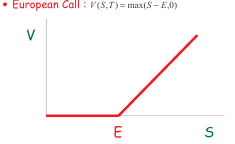
\includegraphics[width=0.4\textwidth]{media2/media/image55.png}
    \caption{Payoff diagram of a European Call option at expiration showing option value $V(S,T)$ as a function of the underlying stock price $S$. The value is zero for stock prices below the strike price $E$, and increases linearly for $S > E$ \cite{bergara2011finite}.}
    \label{fig:your_label_name}
\end{figure}

\subhead{European Put Option}

The payoff function is:
\begin{equation}
    V(S,T) = \max(E - S,0)
\end{equation}

\noindent \textbf{Interpretation:}
\begin{itemize}
    \item If the stock price goes below the strike price, the put option will become profitable.
    \item If the stock price exceeds the strike price, the option expires worthless.
\end{itemize}

\noindent \textbf{Graph Behavior:}
The payoff decreases linearly as the stock price increases and becomes zero after the strike price. These payoff diagrams demonstrate the opposite nature of call and put options.

\begin{figure}[H]
    \centering
    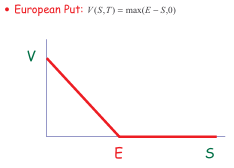
\includegraphics[width=0.4\textwidth]{media2/media/image56.png}
    \caption{Payoff diagram of a European Put option at maturity showing option value $V(S,T)$ as a function of the underlying stock price $S$. The option value decreases linearly for stock prices below the strike price $E$, and is zero for $S > E$ \cite{bergara2011finite}.}
    \label{fig:your_label_name}
\end{figure}

% ------------------------------------------
\subsection{Binary (Digital) Options}
% ------------------------------------------

\begin{figure}[H]
    \centering
    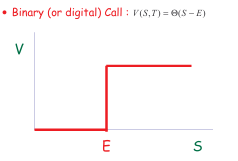
\includegraphics[width=0.4\textwidth]{media2/media/image57.png}
    \caption{Payoff diagram of a Binary (or digital) Call option at expiration showing a step function $V(S,T) = \Theta(S-E)$. The payoff is zero when the asset price $S$ is below the strike price $E$, and jumps discontinuously to a fixed constant value for $S > E$ \cite{bergara2011finite}. }
    \label{fig:your_label_name}
\end{figure}

\subhead{Binary (Digital) call Option}

The payoff is:
\begin{equation}
    V(S,T) = \theta(S - E)
\end{equation}
Where $\theta$ represents the step function.

\noindent \textbf{Interpretation:}
\begin{itemize}
    \item The option pays a fixed amount if the stock price remains below the strike price.
    \item Otherwise, the payoff is zero.
\end{itemize}

\noindent \textbf{Graph Behavior:}
The graph remains constant below the strike price and suddenly drops to zero afterward.

\begin{figure}[H]
    \centering
    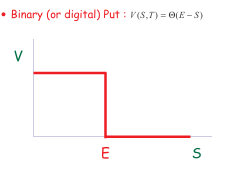
\includegraphics[width=0.4\textwidth]{media2/media/image58.png}
    \caption{Payoff diagram of a Binary (or digital) Put option at expiration showing a step function $V(S,T) = \Theta(E-S)$. The payoff is a fixed constant value when the asset price $S$ is below the strike price $E$, and drops to zero for $S > E$ \cite{bergara2011finite}.}
    \label{fig:your_label_name}
\end{figure}

% ------------------------------------------
\subsection{Bull and Bear Spreads}
% ------------------------------------------

\subhead{Bull spread}

The payoff function for a bull spread is:
\begin{equation}
    V(S,T) = \max\left( S - E_{1},0 \right) - \max\left( S - E_{2},0 \right)
\end{equation}
with $E_{1} < E_{2}$.

\noindent \textbf{Interpretation:}
A bull spread is designed for investors who expect the stock price to rise moderately. The strategy is formed by:
\begin{itemize}
    \item purchasing a call option with strike price $E_{1}$.
    \item Selling another call option with higher strike price $E_{2}$.
\end{itemize}

\noindent \textbf{Payoff Characteristics:}
\begin{itemize}
    \item When $S > E_{1}$, both options expire worthless and the payoff is zero.
    \item Between $E_{1}$ and $E_{2}$, the payoff increases linearly.
    \item After $E_{2}$ the profit becomes constant because gains from the purchased option are offset by losses from the sold option.
\end{itemize}

\noindent \textbf{Financial Significance:}
The bull spread:
\begin{itemize}
    \item limits maximum profit,
    \item reduces trading cost,
    \item and controls downside risk.
\end{itemize}
It is suitable when moderate upward movement in the asset price is expected.

\begin{figure}[H]
    \centering
    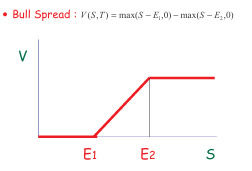
\includegraphics[width=0.45\textwidth]{media2/media/image59.png}
    \caption{Payoff diagram of a Bull Spread strategy at expiration using two strike prices $E_1 < E_2$. The option value is zero for $S \le E_1$, increases linearly between $E_1$ and $E_2$, and reaches a constant maximum profit for $S \ge E_2$ \cite{bergara2011finite}.}
    \label{fig:your_label_name}
\end{figure}

\subhead{Bear Spread}

The payoff function for a bear spread is:
\begin{equation}
    V(S,T) = \max\left( E_{2} - S,0 \right) - \max\left( E_{1} - S,0 \right)
\end{equation}

\noindent \textbf{Interpretation:}
A bear spread is used when an investor expects the stock price to decline moderately. This strategy is formed using put options with different strike prices.

\noindent \textbf{Payoff Characteristics:}
\begin{itemize}
    \item When the stock price is low the payoff is highest .
    \item As stock price rises, the payoff decreases.
\end{itemize}
Beyond the higher strike price, the payoff becomes zero.

\noindent \textbf{Financial Significance:}
The bear spread:
\begin{itemize}
    \item profits from falling prices,
    \item limits losses,
    \item and reduces the initial investment compared with buying a single put option.
\end{itemize}

\begin{figure}[H]
    \centering
    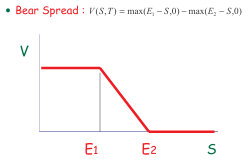
\includegraphics[width=0.45\textwidth]{media2/media/image60.png}
    \caption{Payoff diagram of a Bear Spread strategy at expiration using two strike prices $E_1 < E_2$. The option value is at its maximum constant profit for $S \le E_1$, decreases linearly between $E_1$ and $E_2$, and is zero for $S \ge E_2$ \cite{bergara2011finite}.}
    \label{fig:your_label_name}
\end{figure}

% ------------------------------------------
\subsection{Straddle and Strangle}
% ------------------------------------------

Such approaches are typically employed when investors expect significant price changes but are unsure of the direction of such changes.

\subhead{Straddle}

The straddle consists of:
\begin{itemize}
    \item one call option.
    \item and one put option.
\end{itemize}
With the same strike price $E$.

\noindent \textbf{Payoff Behavior:}
The payoff graph forms a ``V'' shape.
\begin{itemize}
    \item If the stock price moves significantly upward, the call option becomes profitable.
    \item If the stock price falls sharply, the put option becomes profitable.
    \item Maximum loss occurs near the strike price.
\end{itemize}

\noindent \textbf{Financial Interpretation:}
A straddle benefits from:
\begin{itemize}
    \item high market volatility,
    \item Large price movements in either direction.
\end{itemize}
It is commonly used before important market events where large fluctuations are expected.

\begin{figure}[H]
    \centering
    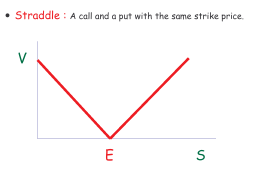
\includegraphics[width=0.45\textwidth]{media2/media/image61.png}
    \caption{Payoff diagram of a Straddle strategy at expiration combining a call and a put with the same strike price $E$. The V-shaped payoff shows higher profits for large asset price movements in either direction, with the minimum value at $S = E$ \cite{bergara2011finite}.}
    \label{fig:your_label_name}
\end{figure}

\subhead{Strangle}

A strangle is similar to a straddle but uses different strike prices:
\begin{itemize}
    \item the put option has a lower strike $E_{1}$.
    \item the call option has a higher strike $E_{2}$.
\end{itemize}

\noindent \textbf{Payoff Behavior:}
The payoff remains near zero between the two strike prices and increases outside this region.

\noindent \textbf{Financial Interpretation:}
Compared with a straddle:
\begin{itemize}
    \item the initial cost is lower,
    \item but larger price movement is required to generate profit.
\end{itemize}
The strategy is appropriate when extreme market volatility is expected.

\begin{figure}[H]
    \centering
    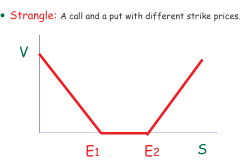
\includegraphics[width=0.45\textwidth]{media2/media/image62.png}
    \caption{Payoff diagram of a Strangle strategy at expiration combining a call and a put with different strike prices $E_1 < E_2$. The payoff is zero in the region $[E_1, E_2]$ and increases linearly outside this interval as price deviates significantly \cite{bergara2011finite}.}
    \label{fig:your_label_name}
\end{figure}

% ------------------------------------------
\subsection{Butterfly and Condor Strategies}
% ------------------------------------------

This page discusses more advanced option combinations used to profit from low volatility and stable market conditions.

\begin{figure}[H]
    \centering
    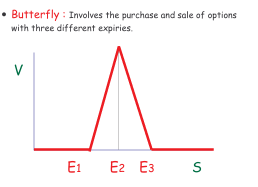
\includegraphics[width=0.45\textwidth]{media2/media/image63.png}
    \caption{Payoff diagram of a Butterfly Spread strategy at expiration using three strike prices $E_1 < E_2 < E_3$. The payoff forms a triangular peak reaching its maximum value at the middle strike price $E_2$, and drops to zero for $S \le E_1$ and $S \ge E_3$ \cite{bergara2011finite}.}
    \label{fig:your_label_name}
\end{figure}

\subhead{Butterfly Spread}

A butterfly strategy combines options with three strike prices:
\begin{equation*}
    E_{1} < E_{2} < E_{3}
\end{equation*}

\noindent \textbf{Payoff Characteristics:}
\begin{itemize}
    \item The payoff reaches its maximum near the middle strike price $E_{2}$.
    \item Losses occur when the stock price moves too far upward or downward.
    \item The graph resembles a tent or triangular peak.
\end{itemize}

The butterfly spread is suitable when:
\begin{itemize}
    \item the investor expects the stock price to remain close to a target value,
    \item and market volatility is expected to remain low.
\end{itemize}

This strategy provides:
\begin{itemize}
    \item limited profit,
    \item limited risk,
    \item and relatively low cost.
\end{itemize}

\subhead{Condor Spread}

The condor spread extends the butterfly strategy by using four strike prices:
\begin{equation*}
    E_{1} < E_{2} < E_{3} < E_{4}
\end{equation*}

\noindent \textbf{Payoff Characteristics:}
\begin{itemize}
    \item The payoff reaches a flat maximum region between the middle strikes.
    \item Profit remains stable over a wider range of prices compared with the butterfly spread.
\end{itemize}

\noindent \textbf{Financial Interpretation:}
The condor strategy:
\begin{itemize}
    \item provides a broader profitable region,
    \item reduces sensitivity to small price changes,
    \item and is useful in stable market environments.
\end{itemize}

\begin{figure}[H]
    \centering
    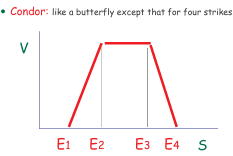
\includegraphics[width=0.45\textwidth]{media2/media/image64.png}
    \caption{Payoff diagram of a Condor Spread strategy at expiration using four strike prices $E_1 < E_2 < E_3 < E_4$. The payoff has a flat maximum region of constant profit between $E_2$ and $E_3$, and drops to zero for $S \le E_1$ and $S \ge E_4$ \cite{bergara2011finite}.}
    \label{fig:your_label_name}
\end{figure}

% ==========================================
\section{Transformation to Constant Coefficient Diffusion Equation}
% ==========================================

The Black--Scholes equation can be simplified mathematically through a change of variables. The evolution converts the Black--Scholes PDE into the standard heat diffusion equation.

The substitution is written as:
\begin{equation}
    V(S,t) = e^{\alpha x + \beta\tau}U(x,\tau)
\end{equation}

Where:
\begin{itemize}
    \item $x = \log S$,
    \item $\tau$ is a transformed time variable.
\end{itemize}

\subhead{Purpose of the Transformation}

The original Black--Scholes model include variable coefficients that complicate analysis and numerical computation.
\begin{equation*}
    \pd{V}{t} + \frac{1}{2}\sigma^{2}S^{2}\pdd{V}{S} + rS\pd{V}{S} - rV = 0
\end{equation*}

After transformation, the PDE becomes:
\begin{equation*}
    \pd{U}{\tau} = \pdd{U}{x}
\end{equation*}
that is the standard heat equation.

\subhead{Reverse the Time Variable}

Define a new time variable:
\begin{equation}
    \tau = T - t
\end{equation}
Where:
\begin{itemize}
    \item $T = \text{maturity time}$,
    \item $\tau = \text{remaining time until expiry}$.
\end{itemize}

Since $\tau = T - t$, then:
\begin{equation*}
    \pd{V}{t} = - \pd{V}{\tau}
\end{equation*}

Substitute into the PDE:
\begin{equation*}
    - \pd{V}{\tau} + \frac{1}{2}\sigma^{2}S^{2}\pdd{V}{S} + rS\pd{V}{S} - rV = 0
\end{equation*}
Rearranging:
\begin{equation}
    \pd{V}{\tau} = \frac{1}{2}\sigma^{2}S^{2}\pdd{V}{S} + rS\pd{V}{S} - rV
\end{equation}

\subhead{Transform the Stock Variable}

Introduce the logarithmic variable:
\begin{equation}
    x = \ln\left( \frac{S}{E} \right)
\end{equation}
Where $E$ is the strike price. Then:
\begin{equation*}
    S = Ee^{x}
\end{equation*}
This transformation simplifies derivatives involving $S^{2}$.

\noindent \textbf{Convert the Derivatives:}
We now express derivatives with respect to $S$ in terms of $x$.

\noindent \textbf{First Derivative:}
Since $x = \ln\left( \frac{S}{E} \right)$, then:
\begin{equation*}
    \frac{dx}{dS} = \frac{1}{S}
\end{equation*}
Now we use the chain rule:
\begin{equation*}
    \pd{V}{S} = \pd{V}{x}\pd{x}{S}
\end{equation*}
Therefore:
\begin{equation}
    \pd{V}{S} = \frac{1}{S}V_{x}
\end{equation}

\noindent \textbf{Second derivative:}
Differentiate again:
\begin{equation*}
    \pdd{V}{S} = \pd{}{S}\left( \frac{1}{S}V_{x} \right)
\end{equation*}
Apply product rule:
\begin{equation*}
    = - \frac{1}{S^{2}}V_{x} + \frac{1}{S}\pd{V_{x}}{S}
\end{equation*}
Using the chain rule again:
\begin{equation*}
    \pd{V_{x}}{S} = \frac{1}{S}V_{xx}
\end{equation*}
Therefore:
\begin{equation*}
    \pdd{V}{S} = - \frac{1}{S^{2}}V_{x} + \frac{1}{S^{2}}V_{xx}
\end{equation*}
Thus:
\begin{equation}
    \pdd{V}{S} = \frac{1}{S^{2}}(V_{xx} - V_{x})
\end{equation}

\subhead{Substitute into the PDE}

Substitute derivatives into:
\begin{equation*}
    \pd{V}{\tau} = \frac{1}{2}\sigma^{2}S^{2}\pdd{V}{S} + rS\pd{V}{S} - rV
\end{equation*}

Using:
\begin{equation*}
    \pdd{V}{S} = \frac{1}{S^{2}}(V_{xx} - V_{x}) \quad \text{and} \quad \pd{V}{S} = \frac{1}{S}V_{x}
\end{equation*}

We obtain:
\begin{equation*}
    V_{\tau} = \frac{1}{2}\sigma^{2}\left( V_{xx} - V_{x} \right) + rV_{x} - rV
\end{equation*}

Expand:
\begin{equation*}
    V_{\tau} = \frac{1}{2}\sigma^{2}V_{xx} - \frac{1}{2}\sigma^{2}V_{x} + rV_{x} - rV
\end{equation*}

Combine the $V_{x}$ terms:
\begin{equation}
    V_{\tau} = \frac{1}{2}\sigma^{2}V_{xx} + \left( r - \frac{1}{2}\sigma^{2} \right)V_{x} - rV
\end{equation}

\subhead{Remove First Derivative and Reaction Terms}

We now transform: $V(x,\tau) = e^{\alpha x + \beta\tau}U(x,\tau)$

\noindent \textbf{Compute Derivatives:}

\noindent Time Derivative:
\begin{equation*}
    V_{\tau} = e^{\alpha x + \beta\tau}(U_{\tau} + \beta U)
\end{equation*}
\noindent First Space Derivative:
\begin{equation*}
    V_{x} = e^{\alpha x + \beta\tau}(U_{x} + \alpha U)
\end{equation*}
\noindent Second Space Derivative:
\begin{equation*}
    V_{xx} = e^{\alpha x + \beta\tau}(U_{xx} + 2\alpha U_{x} + \alpha^{2}U)
\end{equation*}

\noindent \textbf{Substitute again:}
Substitute into:
\begin{equation*}
    V_{\tau} = \frac{1}{2}\sigma^{2}V_{xx} + \left( r - \frac{1}{2}\sigma^{2} \right)V_{x} - rV
\end{equation*}

Factor out $e^{\alpha x + \beta\tau}$. After substitution:
\begin{equation*}
    U_{\tau} + \beta U = \frac{1}{2}\sigma^{2}\left( U_{xx} + 2\alpha U_{x} + \alpha^{2}U \right) + \left( r - \frac{1}{2}\sigma^{2} \right)\left( U_{x} + \alpha U \right) - rU
\end{equation*}

Expand:
\begin{equation*}
    U_{\tau} + \beta U = \frac{1}{2}\sigma^{2}U_{xx} + \sigma^{2}\alpha U_{x} + \frac{1}{2}\sigma^{2}\alpha^{2}U + \left( r - \frac{1}{2}\sigma^{2} \right)U_{x} + \alpha\left( r - \frac{1}{2}\sigma^{2} \right)U - rU
\end{equation*}

\noindent \textbf{Eliminate the $U_{x}$ term:}
Coefficient of $U_{x}$:
\begin{equation*}
    \sigma^{2}\alpha + r - \frac{1}{2}\sigma^{2}
\end{equation*}
Set equal to zero:
\begin{equation*}
    \sigma^{2}\alpha + r - \frac{1}{2}\sigma^{2} = 0
\end{equation*}
Solve for $\alpha$:
\begin{equation}
    \alpha = \frac{1}{2} - \frac{r}{\sigma^{2}}
\end{equation}

\noindent \textbf{Eliminate the $U$ term:}
Coefficient of $U$:
\begin{equation*}
    \frac{1}{2}\sigma^{2}\alpha^{2} + \alpha\left( r - \frac{1}{2}\sigma^{2} \right) - r - \beta = 0
\end{equation*}

Choose $\beta$ so it equals zero. After simplification:
\begin{equation}
    \beta = -\frac{1}{2}\sigma^{2}\left( \frac{r}{\sigma^{2}} + \frac{1}{2} \right)^{2}
\end{equation}

\noindent \textbf{Final Simplified Equation:}
The PDE reduces to:
\begin{equation}
    U_{\tau} = \frac{1}{2}\sigma^{2}U_{xx}
\end{equation}
This is the classical heat diffusion equation.

\subhead{Solve the Heat Equation}

The solution is the Gaussian kernel:
\begin{equation}
    U(x,\tau) = \frac{1}{\sqrt{2\pi\sigma^{2}\tau}}\int_{- \infty}^{\infty}e^{- \frac{(x - y)^{2}}{2\sigma^{2}\tau}}f(y)dy
\end{equation}
Where $f(y)$ is the payoff function. This represents diffusion of the payoff through time.

\noindent \textbf{Apply the European Call Payoff:}
For a European call option:
\begin{equation*}
    V(S,T) = \max(S - E,0)
\end{equation*}

Substituting this payoff into the integral solution and simplifying gives the Black--Scholes formula.

\noindent \textbf{Final Black--Scholes Formula:}
The European call price becomes:
\begin{equation}
    C(S,t) = SN(d_{1}) - Ee^{- r(T - t)}N(d_{2})
\end{equation}
Where:
\begin{align}
    d_{1} &= \frac{\ln\left( \frac{S}{E} \right) + \left( r + \frac{1}{2}\sigma^{2} \right)(T - t)}{\sigma\sqrt{T - t}} \\
    d_{2} &= d_{1} - \sigma\sqrt{T - t}
\end{align}

\noindent \textbf{European Put Formula:}
Similarly:
\begin{equation}
    P(S,t) = Ee^{- r(T - t)}N( - d_{2}) - SN( - d_{1})
\end{equation}

% ==========================================
\section{Extensions of the Black--Scholes Equation}
% ==========================================

This portion represents several important extensions of standard Black--Scholes model. These extensions allow the pricing framework to be applied to a greater variety of financial derivatives and more realistic market conditions. By modifying the original Black--Scholes partial differential equation (PDE), the model can incorporate dividends, foreign exchange markets, commodities, futures contracts, stochastic interest rates, and other complex financial instruments.

\subhead{I. Options on Dividend-Paying Equities}

In the standard Black--Scholes model, the underlying asset is assumed not to pay dividends. However, many real-world stocks distribute dividends continuously over time. Let $D$ denote the constant dividend yield.

The modified Black--Scholes equation becomes:
\begin{equation}
    \pd{V}{t} + \frac{1}{2}\sigma^{2}S^{2}\pdd{V}{S} + (r - D)S\pd{V}{S} - rV = 0
\end{equation}

\noindent \textbf{Interpretation:}
The dividend yield reduces the effective growth rate of the stock price because part of the asset value is distributed to shareholders. Consequently, dividend payments decreases the prices of call option and increase the put option prices relative to the standard model.

\subhead{II. Currency Options}

Currency options are options written on foreign exchange rates. In this case, holding foreign currency generates interest at the foreign risk-free interest rate $r_{f}$.

The governing PDE becomes:
\begin{equation}
    \pd{V}{t} + \frac{1}{2}\sigma^{2}S^{2}\pdd{V}{S} + \left( r - r_{f} \right)S\pd{V}{S} - rV = 0
\end{equation}

\noindent \textbf{Interpretation:}
The foreign interest rate acts similarly to a dividend yield because investors holding foreign currency receive interest payments. Therefore, the pricing structure resembles the dividend-paying equity model.

\subhead{III. Commodity Options}

Commodity options differ from stock options because commodities involve storage expenses and carrying costs. These additional costs are represented by the parameter $q$, known as the cost of carry.

The modified PDE is:
\begin{equation}
    \pd{V}{t} + \frac{1}{2}\sigma^{2}S^{2}\pdd{V}{S} + (r + q)S\pd{V}{S} - rV = 0
\end{equation}

\noindent \textbf{Interpretation:}
The cost of carry increases the effective growth rate of the commodity price. This extension is commonly used in pricing options on oil, gold, agricultural products, and other physical commodities.

\subhead{IV. Options on Futures}

Options can also be written on futures contracts rather than directly on the spot asset price. The futures price $F$ for a non-dividend-paying asset is related to the spot price by:
\begin{equation*}
    F = e^{r(T - t)}S
\end{equation*}

Using this transformation, the Black--Scholes equation reduces to:
\begin{equation}
    \pd{U}{t} + \frac{1}{2}\sigma^{2}F^{2}\pdd{U}{F} - rU = 0
\end{equation}

\noindent \textbf{Interpretation:}
Since futures contracts already incorporate financing effects, the drift term disappears from the equation, simplifying the pricing model.

\subhead{V. Options on Time-Dependent Parameters}

The standard Black-Scholes model suppose constant volatility and interest rates. In practice, however, these parameters often vary with time.

The generalized PDE becomes:
\begin{equation}
    \pd{V}{t} + \frac{1}{2}\sigma(t)^{2}S^{2}\pdd{V}{S} + \left[ r(t) - D(t) \right] S\pd{V}{S} - r(t)V = 0
\end{equation}

\noindent \textbf{Interpretation:}
This extension makes financial markets more realistic by enabling:
\begin{itemize}
    \item volatility to change over time,
    \item interest rates to fluctuate,
    \item and dividend yields to vary.
\end{itemize}
Such models are widely used in practical financial engineering.

\subhead{VI. Power Options}

Power options are exotic derivatives whose payoff depends on the asset price raised to a power $\alpha$. If:
\begin{equation*}
    P = S^{\alpha}
\end{equation*}

Then the corresponding PDE becomes:
\begin{equation}
    \pd{V}{t} + \frac{1}{2}\alpha^{2}\sigma^{2}P^{2}\pdd{V}{P} + \alpha\left[ \frac{1}{2}\sigma^{2}(\alpha - 1) + r \right] P\pd{V}{P} - rV = 0
\end{equation}

\noindent \textbf{Interpretation:}
Power options magnify the effect of price movements through the exponent $\alpha$. They are used in specialized financial products and structured derivatives.

\subhead{VII. Two-Factor Options}

In some advanced financial models, both the asset price and the interest rate are treated as stochastic variables.

The interest rate process is assumed to satisfy:
\begin{equation*}
    dr = u(r,t)dt + w(r,t)dX
\end{equation*}

Under this assumption, the option value satisfies a two-factor PDE:
\begin{equation}
    \pd{V}{t} + \frac{1}{2}\sigma^{2}S^{2}\pdd{V}{S} + \frac{1}{2}w^{2}\pdd{V}{r} + rS\pd{V}{S} + (\mu - \lambda w)\pd{V}{r} - rV = 0
\end{equation}

\noindent \textbf{Interpretation:}
This model incorporates uncertainty in both:
\begin{itemize}
    \item asset prices,
    \item and interest rates.
\end{itemize}
Such equations are important in pricing interest-rate-sensitive derivatives and fixed-income securities.

\subhead{VIII. Early Exercise Options}

American and Bermudan options allow exercise before maturity, unlike European options which can only be exercised at expiration.

\noindent \textbf{Interpretation:}
For early exercise options:
\begin{itemize}
    \item the exercise boundary is unknown,
    \item the pricing problem becomes more complex,
    \item and free-boundary methods are usually required.
\end{itemize}

The valuation of these options often involves numerical methods such as:
\begin{itemize}
    \item finite difference methods,
    \item binomial trees,
    \item and variational inequality techniques.
\end{itemize}

% ==========================================
\section{Finite Difference Methods for the Black--Scholes Equation}
% ==========================================

The Black--Scholes PDE can be solved numerically using finite difference methods. Numerical approximation techniques are crucial in computational finance because many financial derivatives lack closed-form analytical answers. The continuous Black-Scholes PDE is transformed into a discrete algebraic problem that can be solved on a computing grid using the finite difference method.

\subhead{Introduction to the Black--Scholes Equation}

The Black--Scholes PDE for a European option is:
\begin{equation}
    \pd{V}{t} + \frac{1}{2}\sigma^{2}S^{2}\pdd{V}{S} + rS\pd{V}{S} - rV = 0
\end{equation}

Where:
\begin{itemize}
    \item $V(S,t) = \text{option value}$
    \item $S = \text{stock price}$
    \item $t = \text{time}$
    \item $r = \text{risk free interest rate}$
    \item $\sigma = \text{volatility}$
\end{itemize}

\subhead{Error Analysis}

Finite difference approximations replace derivatives with algebraic formulas. This introduces truncation errors. For example:
\begin{equation*}
    \mathcal{O}(\Delta t, \Delta S^{2})
\end{equation*}

Means:
\begin{itemize}
    \item First-order accuracy in time.
    \item Second-order accuracy in space.
\end{itemize}

\subhead{Stability Restrictions}

Some numerical methods become unstable if:
\begin{itemize}
    \item Time step becomes too large
    \item Grid spacing becomes inappropriate
\end{itemize}

An unstable method produces:
\begin{itemize}
    \item Oscillations
    \item Diverging solutions
    \item Numerical explosion
\end{itemize}

Explicit schemes are conditionally stable. Implicit schemes are usually unconditionally stable.

\subhead{Computational Speed}

Large numerical grids create:
\begin{itemize}
    \item Large matrices
    \item Many calculations
    \item High memory requirements
\end{itemize}

Efficient numerical schemes are essential in financial engineering.

\subhead{Flexibility of the Method}

Financial models frequently change because of:
\begin{itemize}
    \item American options
    \item Barrier options
    \item Dividend payments
    \item Free boundaries
    \item Variable volatility
\end{itemize}

A good numerical method should adapt easily.

% ==========================================
\subsection{Explicit Finite Difference Method}
% ==========================================

\noindent \textbf{PDE:}
Start with the simplified form (like the heat equation after transformation):
\begin{equation}
    \pd{V}{t} = \pdd{V}{S}
\end{equation}

\noindent \textbf{Grid Definition:}
Define:
\begin{equation*}
    S_{n} = n\Delta S \quad \text{and} \quad t_{m} = m\Delta t
\end{equation*}

Where:
\begin{itemize}
    \item $n = \text{spatial index}$
    \item $m = \text{time index}$
\end{itemize}

Approximate solution:
\begin{equation*}
    V_{n}^{m} \approx V(S_{n},t_{m})
\end{equation*}

\noindent \textbf{Forward Difference in Time:}
Approximate the time derivative:
\begin{equation}
    \pd{V}{t} \approx \frac{V_{n}^{m + 1} - V_{n}^{m}}{\Delta t}
\end{equation}
This is first-order accurate.

\noindent \textbf{Central Difference in Space:}
Approximate the second derivative:
\begin{equation}
    \pdd{V}{S} \approx \frac{V_{n + 1}^{m} - 2V_{n}^{m} + V_{n - 1}^{m}}{\Delta S^{2}}
\end{equation}
This is second-order accurate.

Substitute both approximations:
\begin{equation*}
    \frac{V_{n}^{m + 1} - V_{n}^{m}}{\Delta t} = \frac{V_{n + 1}^{m} - 2V_{n}^{m} + V_{n - 1}^{m}}{\Delta S^{2}}
\end{equation*}

Multiply by $\Delta t$:
\begin{equation*}
    V_{n}^{m + 1} = V_{n}^{m} + \frac{\Delta t}{\Delta S^{2}}\left( V_{n + 1}^{m} - 2V_{n}^{m} + V_{n - 1}^{m} \right)
\end{equation*}

Define:
\begin{equation*}
    \lambda = \frac{\Delta t}{\Delta S^{2}}
\end{equation*}

Then:
\begin{equation}
    V_{n}^{m + 1} = \lambda V_{n + 1}^{m} + (1 - 2\lambda)V_{n}^{m} + \lambda V_{n - 1}^{m}
\end{equation}

\subhead{Properties of Explicit Method}

\begin{table}[H]
    \centering
    \begin{tabular}{ll}
        \toprule
        \textbf{Property} & \textbf{Description} \\
        \midrule
        Time Accuracy & First-order \\
        Space Accuracy & Second-order \\
        Stability & Conditional \\
        Complexity & Simple \\
        Speed & Fast per step \\
        \bottomrule
    \end{tabular}
    \caption{Properties of the Explicit Method}
\end{table}

\subhead{Stability Condition}

Explicit schemes require:
\begin{equation*}
    \lambda \leq \frac{1}{2}
\end{equation*}
Which means:
\begin{equation}
    \frac{\Delta t}{\Delta S^{2}} \leq \frac{1}{2}
\end{equation}
Therefore, small time steps are necessary.

% ==========================================
\subsection{Fully Implicit Method}
% ==========================================

In the fully implicit method all spatial derivatives are computed at the new time level $m + 1$.

\subhead{Grid Discretization}

The computational region is divided into stock price intervals and time intervals.
Define:
\begin{align*}
    S_{i} &= i\Delta S, \quad i = 0,1,\dots,M \\
    t_{j} &= j\Delta t, \quad j = 0,1,\dots,N
\end{align*}

The numerical approximation is:
\begin{equation*}
    V_{i,j} \approx V(S_{i},t_{j})
\end{equation*}

\noindent \textbf{Backward Difference Time Derivative:}
For the implicit method:
\begin{equation}
    \pd{V}{t} \approx \frac{V_{i,j + 1} - V_{i,j}}{\Delta t}
\end{equation}

\noindent \textbf{Central difference Second Spatial Derivative:}
\begin{equation}
    \pdd{V}{S} \approx \frac{V_{i + 1,j + 1} - 2V_{i,j + 1} + V_{i - 1,j + 1}}{\Delta S^{2}}
\end{equation}

\noindent \textbf{Central difference First Spatial Derivative:}
\begin{equation}
    \pd{V}{S} \approx \frac{V_{i + 1,j + 1} - V_{i - 1,j + 1}}{2\Delta S}
\end{equation}

Substitute finite differences into the PDE:
\begin{equation*}
    \frac{V_{i,j + 1} - V_{i,j}}{\Delta t} + \frac{1}{2}\sigma^{2}S_{i}^{2}\frac{V_{i + 1,j + 1} - 2V_{i,j + 1} + V_{i - 1,j + 1}}{\Delta S^{2}} + rS_{i}\frac{V_{i + 1,j + 1} - V_{i - 1,j + 1}}{2\Delta S} - rV_{i,j + 1} = 0
\end{equation*}

\subhead{Introduce Mesh Ratios}

Define:
\begin{equation*}
    v_{1} = \frac{\Delta t}{\Delta S^{2}} \quad \text{and} \quad v_{2} = \frac{\Delta t}{\Delta S}
\end{equation*}

Collect coefficients of $V_{i - 1,j + 1}$, $V_{i,j + 1}$, and $V_{i + 1,j + 1}$. Then:
\begin{equation}
    - A_{i}V_{i - 1,j + 1} + \left( 1 + B_{i} \right)V_{i,j + 1} - C_{i}V_{i + 1,j + 1} = V_{i,j}
\end{equation}

Where:
\begin{align}
    A_{i} &= \frac{1}{2}v_{1}\sigma^{2}i^{2} - \frac{1}{2}v_{2}ri \\
    B_{i} &= v_{1}\sigma^{2}i^{2} + r\Delta t \\
    C_{i} &= \frac{1}{2}v_{1}\sigma^{2}i^{2} + \frac{1}{2}v_{2}ri
\end{align}

\subhead{Matrix Form}

The implicit method generates a tridiagonal matrix system:
\begin{equation}
    M V^{j + 1} = V^{j}
\end{equation}

Where:
\begin{itemize}
    \item $M$ is a tridiagonal coefficient matrix,
    \item $V^{j}$ is the known vector at the current time level,
    \item $V^{j + 1}$ is the unknown vector at the next time level.
\end{itemize}

\subhead{Local Truncation Error}

The scheme has error:
\begin{equation*}
    \mathcal{O}(\Delta t, \Delta S^{2})
\end{equation*}
Meaning:
\begin{itemize}
    \item First-order accurate in time.
    \item Second-order accurate in space.
\end{itemize}

\subhead{Stability of the Implicit Method}

The implicit method is:
\begin{itemize}
    \item Unconditionally stable.
    \item Much more reliable than the explicit method.
\end{itemize}
This means large time steps may be used safely.

\subhead{Properties of Implicit Method}

\begin{table}[H]
    \centering
    \begin{tabular}{ll}
        \toprule
        \textbf{Property} & \textbf{Description} \\
        \midrule
        Stability & Unconditionally stable \\
        Time Accuracy & First-order \\
        Space Accuracy & Second-order \\
        Complexity & Requires matrix solution \\
        \bottomrule
    \end{tabular}
    \caption{Properties of the Implicit Method}
\end{table}

% ==========================================
\subsection{Numerical Implementation}
% ==========================================

The Black--Scholes partial differential equation was solved numerically using two finite difference schemes:
\begin{itemize}
    \item Explicit Method
    \item Fully Implicit Method
\end{itemize}

MATLAB programs were developed for each numerical scheme in order to approximate the value of a European Call Option under different computational mesh sizes. The numerical results were analyzed through both two-dimensional and three-dimensional graphical representations.

\subhead{Explicit Method --- Graph Interpretation}

\begin{figure}[H]
    \centering
    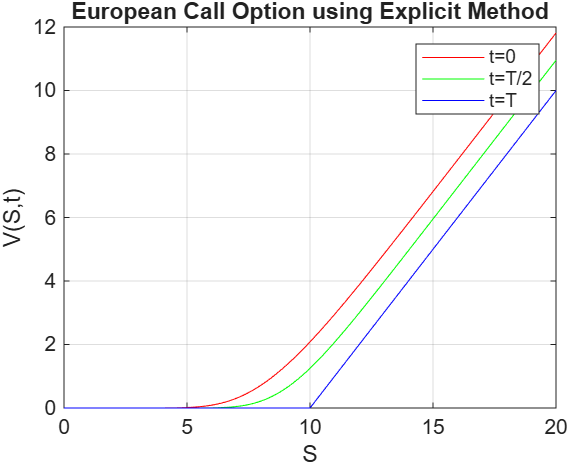
\includegraphics[width=0.7\textwidth]{media2/media/image65.png}
    \caption{Numerical solution for a European Call option valued using the Explicit Finite Difference Method at different times $t=0$, $t=T/2$, and $t=T$. The sharp payoff corner at maturity ($t=T$) at strike price $E=10$ becomes progressively smoother due to diffusion as time moves backward to $t=0$.}
    \label{fig:your_label_name}
\end{figure}

The fig 7.11 results indicate that:
\begin{itemize}
    \item the option value increases as the stock price increases,
    \item the option value approaches zero for very small stock prices,
    \item and the curves become smoother as the solution moves backward in time.
\end{itemize}

The graph also demonstrates the diffusion behavior of the Black--Scholes equation.

\subhead{3D Surface Interpretation}

The surface 7.12 shows that:
\begin{itemize}
    \item the option value rises continuously with stock price,
    \item the option value changes smoothly over time,
    \item and numerically the solution stays stable for sufficiently fine meshes.
\end{itemize}

Explicit Method produces accurate solutions when the stability condition is satisfied.

\begin{figure}[H]
    \centering
    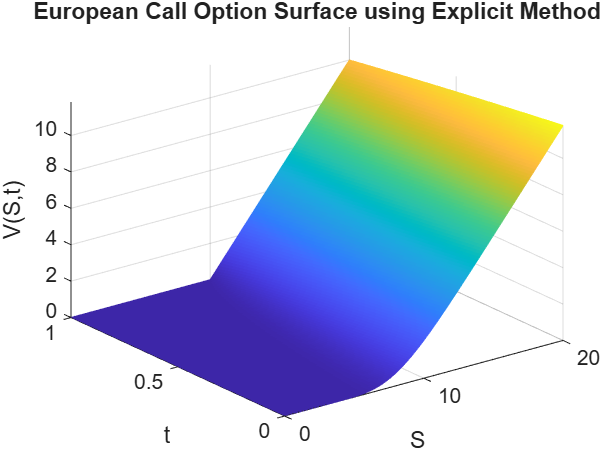
\includegraphics[width=0.7\textwidth]{media2/media/image66.png}
    \caption{Three-dimensional option price surface $V(S,t)$ for a European Call option computed via the Explicit Finite Difference Method over stock price $S \in [0, 20]$ and time $t \in [0, 1]$. The smooth surface demonstrates stable option price evolution over the domain when the stability condition is met.}
    \label{fig:your_label_name}
\end{figure}

\subhead{Fully Implicit Method --- Graph Interpretation}

The Fully Implicit Finite Difference Method was employed to solve the Black--Scholes equation numerically. This method is unconditionally stable and allows us to use  the larger time step sizes.
The graphical results show that:
\begin{itemize}
    \item the option value increases monotonically with stock price,
    \item the numerical solution remains smooth throughout the computational domain,
    \item and no oscillatory behavior is observed.
\end{itemize}


\begin{figure}[H]
    \centering
    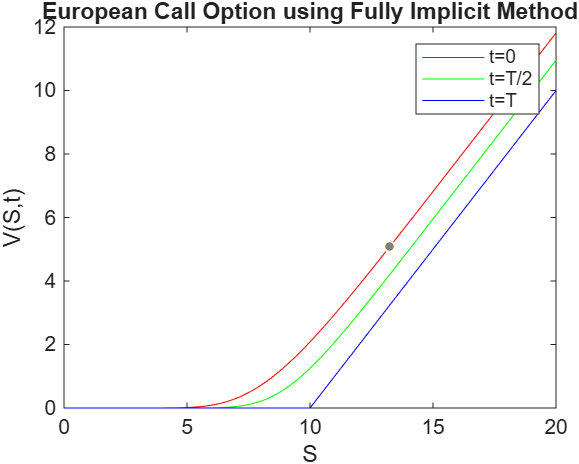
\includegraphics[width=0.7\textwidth]{media2/media/image67.png}
    \caption{Numerical solution for a European Call option valued using the Fully Implicit Method at different times $t=0$, $t=T/2$, and $t=T$ with a strike price $E=10$. The unconditionally stable scheme successfully traces the smooth option value over the asset price domain without oscillations.}
    \label{fig:your_label_name}
\end{figure}

By comparing with Explicit Method, the Fully Implicit Method produces slightly smoother curves because of its diffusive numerical nature.

\subhead{3D Surface}
In fig 7.14 the surface indicates that:
\begin{itemize}
    \item the method remains numerically stable even for coarse meshes,
    \item the option value evolves continuously,
    \item and the numerical damping effect slightly smooths the option surface.
\end{itemize}

The Fully Implicit Method is particularly suitable for large-scale computations due to its unconditional stability.

\begin{figure}[H]
    \centering
    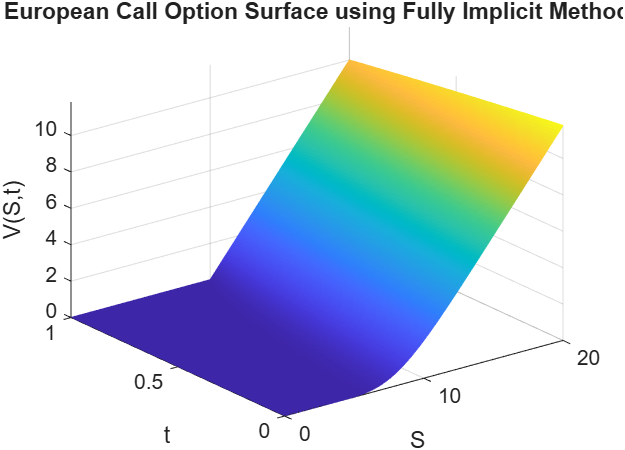
\includegraphics[width=0.8\textwidth]{media2/media/image68.png}
    \caption{Three-dimensional option price surface $V(S,t)$ for a European Call option computed via the Fully Implicit Finite Difference Method over stock price $S \in [0, 20]$ and time $t \in [0, 1]$. The smooth option surface reflects the highly stable, dampening behavior of the implicit approach.}
    \label{fig:your_label_name}
\end{figure}


% ==========================================
\subsection{Derivation of Crank--Nicolson Method}
% ==========================================

The Crank--Nicolson method averages:
\begin{itemize}
    \item Explicit scheme.
    \item Implicit scheme.
\end{itemize}
Thus, it is more accurate.

General weighted form:
\begin{equation}
    \frac{V_{n}^{m + 1} - V_{n}^{m}}{\Delta t} = (1 - \theta)\frac{V_{n + 1}^{m} - 2V_{n}^{m} + V_{n - 1}^{m}}{\Delta S^{2}} + \theta\frac{V_{n + 1}^{m + 1} - 2V_{n}^{m + 1} + V_{n - 1}^{m + 1}}{\Delta S^{2}}
\end{equation}

\subhead{Special Values of Theta}

\begin{table}[H]
    \centering
    \begin{tabular}{ll}
        \toprule
        \textbf{Value of $\theta$} & \textbf{Method} \\
        \midrule
        0 & Explicit \\
        1 & Fully implicit \\
        $1/2$ & Crank-Nicolson \\
        \bottomrule
    \end{tabular}
    \caption{Theta values and corresponding methods}
\end{table}

For $\theta = \frac{1}{2}$, we obtain:
\begin{equation}
    \frac{V_{n}^{m + 1} - V_{n}^{m}}{\Delta t} = \frac{1}{2}\left[ \frac{V_{n + 1}^{m} - 2V_{n}^{m} + V_{n - 1}^{m}}{\Delta S^{2}} + \frac{V_{n + 1}^{m + 1} - 2V_{n}^{m + 1} + V_{n - 1}^{m + 1}}{\Delta S^{2}} \right]
\end{equation}

\subhead{Average Explicit and Implicit Terms}

The PDE is evaluated half at:
\begin{itemize}
    \item Time level $j$.
    \item Time level $j + 1$.
\end{itemize}

The scheme becomes:
\begin{equation*}
    \frac{V_{i,j + 1} - V_{i,j}}{\Delta t} = \frac{1}{2}(LV^{j + 1} + LV^{j})
\end{equation*}
Where $L$ is the Black-Scholes differential operator.

Substitute Finite Differences. After substitution:
\begin{equation}
    - A_{i}V_{i - 1,j + 1} + \left( 1 + B_{i} \right)V_{i,j + 1} - C_{i}V_{i + 1,j + 1} = A_{i}V_{i - 1,j} + \left( 1 - B_{i} \right)V_{i,j} + C_{i}V_{i + 1,j}
\end{equation}

Where:
\begin{align}
    A_{i} &= \frac{1}{4}v_{1}\sigma^{2}i^{2} - \frac{1}{4}v_{2}ri \\
    B_{i} &= \frac{1}{2}v_{1}\sigma^{2}i^{2} + \frac{1}{2}r\Delta t \\
    C_{i} &= \frac{1}{4}v_{1}\sigma^{2}i^{2} + \frac{1}{4}v_{2}ri
\end{align}

\subhead{Matrix Form of Crank--Nicolson Scheme}

The system becomes:
\begin{equation}
    M V^{j + 1} = M^{*}V^{j} + r^{j}
\end{equation}

Where:
\begin{itemize}
    \item $M$ and $M^{*}$ are tridiagonal matrices.
    \item $r^{j}$ contains boundary terms.
\end{itemize}

\subhead{Accuracy of Crank--Nicolson Method}

The truncation error is:
\begin{equation*}
    \mathcal{O}(\Delta t^{2}, \Delta S^{2})
\end{equation*}
Thus it is second-order accurate in time and space.

\subhead{Boundary Conditions}

\noindent \textbf{European Call Option:}

At maturity:
\begin{equation*}
    V(S,T) = \max(S - E,0)
\end{equation*}

Lower Boundary: At $S = 0$:
\begin{equation*}
    V(0,t) = 0
\end{equation*}

Upper Boundary: For large stock prices:
\begin{equation*}
    V(S,t) \approx S - Ee^{- r(T - t)}
\end{equation*}

\subhead{Crank--Nicolson Method --- Graph Interpretation}

Crank--Nicolson Method was implemented as combining the Explicit and Fully Implicit finite difference schemes. This method provides both high accuracy and unconditional stability.

In fig 7.15 the results demonstrate that:
\begin{itemize}
    \item the option value rises with increasing stock price,
    \item the numerical curves remain smooth and stable,
    \item and the approximation near the strike price is more accurate than the Fully Implicit Method.
\end{itemize}

Because the Crank--Nicolson Method is second-order accurate in time, the obtained solution is generally more precise.

\begin{figure}[H]
    \centering
    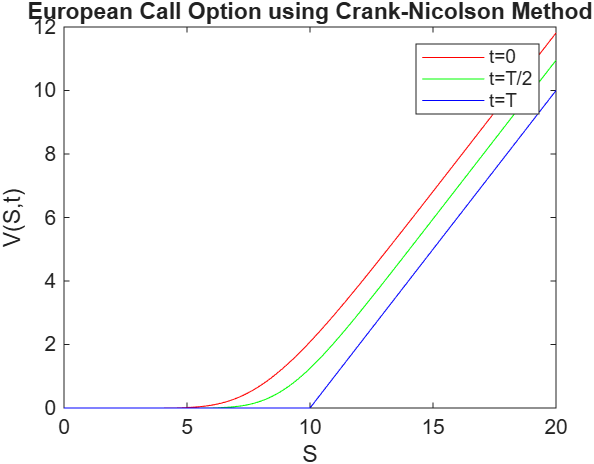
\includegraphics[width=0.8\textwidth]{media2/media/image69.png}
    \caption{Numerical solution for a European Call option valued using the Crank-Nicolson Method at different times $t=0$, $t=T/2$, and $t=T$ with a strike price $E=10$. This second-order accurate method combines high accuracy and unconditional stability for precise option pricing.}
    \label{fig:your_label_name}
\end{figure}

\subhead{3D Surface}

\begin{figure}[H]
    \centering
    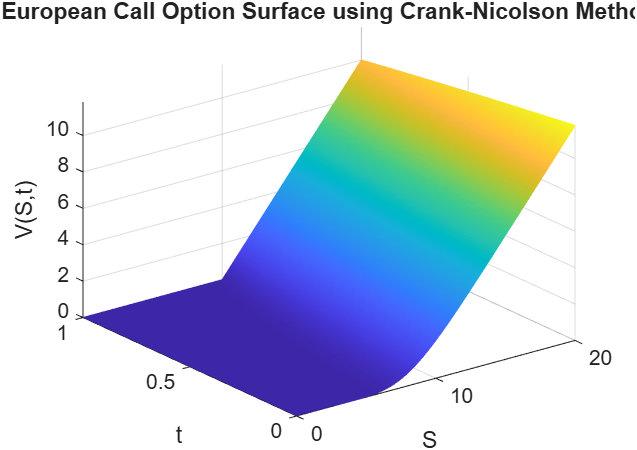
\includegraphics[width=0.8\textwidth]{media2/media/image70.png}
    \caption{Three-dimensional option price surface $V(S,t)$ for a European Call option computed via the Crank-Nicolson Finite Difference Method over stock price $S \in [0, 20]$ and time $t \in [0, 1]$. The surface demonstrates second-order temporal and spatial accuracy and superior resolution near the strike price.}
    \label{fig:your_label_name}
\end{figure}

In fig 7.16 the graphical results indicate:
\begin{itemize}
    \item smooth propagation of the numerical solution,
    \item reduced numerical diffusion,
    \item and accurate approximation of the option price surface.
\end{itemize}

The Crank--Nicolson Method provides a balance between stability and accuracy and is therefore widely used in computational finance.

\subhead{Conclusions}

Although Explicit, Fully Implicit, and Crank--Nicolson methods converge to nearly identical solutions for sufficiently fine grids, their numerical properties differ significantly. The Explicit scheme is conditionally stable and needs very small time steps, whereas the Fully Implicit and Crank--Nicolson schemes are unconditionally stable. Furthermore, the Crank--Nicolson scheme provides higher temporal accuracy and reduced numerical diffusion, making it the most commonly used schemes in computational finance.

% ==========================================
\subsection{Three Time-Level Methods}
% ==========================================

Traditional schemes use two time levels. Three-time-level methods use:
\begin{itemize}
    \item Previous time level
    \item Current time level
    \item Future time level
\end{itemize}
This can improve accuracy.

\subhead{Central Difference in Time}

Approximation:
\begin{equation}
    \frac{V_{n}^{m + 1} - V_{n}^{m - 1}}{2\Delta t} = \frac{V_{n + 1}^{m} - 2V_{n}^{m} + V_{n - 1}^{m}}{\Delta S^{2}}
\end{equation}
This is called the leapfrog method.

Rearrangement: Multiply by $2\Delta t$:
\begin{equation*}
    V_{n}^{m + 1} = V_{n}^{m - 1} + 2\lambda(V_{n + 1}^{m} - 2V_{n}^{m} + V_{n - 1}^{m})
\end{equation*}
Or:
\begin{equation}
    V_{n}^{m + 1} = (1 - 4\lambda)V_{n}^{m} + 2\lambda\left( V_{n + 1}^{m} + V_{n - 1}^{m} \right) + V_{n}^{m - 1}
\end{equation}

\noindent \textbf{Stability Issue:} This scheme is unstable for all time steps. Therefore it is generally not suitable.

\subhead{Dufort--Frankel Method}

To stabilize the method, replace:
\begin{equation*}
    2V_{n}^{m}
\end{equation*}
With:
\begin{equation*}
    V_{n}^{m + 1} + V_{n}^{m - 1}
\end{equation*}

Then:
\begin{equation*}
    \frac{V_{n}^{m + 1} - V_{n}^{m - 1}}{2\Delta t} = \frac{V_{n + 1}^{m} - (V_{n}^{m + 1} + V_{n}^{m - 1}) + V_{n - 1}^{m}}{\Delta S^{2}}
\end{equation*}

Rearrangement of Dufort--Frankel Scheme: Multiply by $2\Delta t$:
\begin{equation*}
    V_{n}^{m + 1} - V_{n}^{m - 1} = 2\lambda\left[ V_{n + 1}^{m} - (V_{n}^{m + 1} + V_{n}^{m - 1}) + V_{n - 1}^{m} \right]
\end{equation*}

Collect terms containing $V_{n}^{m + 1}$:
\begin{equation*}
    (1 + 2\lambda)V_{n}^{m + 1} = 2\lambda\left( V_{n + 1}^{m} + V_{n - 1}^{m} \right) + (1 - 2\lambda)V_{n}^{m - 1}
\end{equation*}

Finally:
\begin{equation}
    V_{n}^{m + 1} = \frac{2\lambda}{1 + 2\lambda}\left( V_{n + 1}^{m} + V_{n - 1}^{m} \right) + \frac{1 - 2\lambda}{1 + 2\lambda}V_{n}^{m - 1}
\end{equation}

\subhead{Properties of Dufort--Frankel Method}

\begin{table}[H]
    \centering
    \begin{tabular}{ll}
        \toprule
        \textbf{Property} & \textbf{Description} \\
        \midrule
        Stability & Unconditionally stable \\
        Accuracy & Lower than Crank--Nicolson \\
        Time Level & Three \\
        \bottomrule
    \end{tabular}
    \caption{Properties of the Dufort-Frankel Method}
\end{table}

\subhead{Richardson Extrapolation}

Richardson extrapolation improves accuracy by combining two numerical solutions.

Suppose:
\begin{align*}
    V_{1} &= V_{\text{exact}} + \epsilon_{1}\Delta t_{1} + \epsilon_{2}\Delta S_{1}^{2} + \dots \\
    V_{2} &= V_{\text{exact}} + \epsilon_{1}\Delta t_{2} + \epsilon_{2}\Delta S_{2}^{2} + \dots
\end{align*}

Choose:
\begin{equation*}
    \frac{\Delta t_{1}}{\Delta S_{1}^{2}} = \frac{\Delta t_{2}}{\Delta S_{2}^{2}}
\end{equation*}
Then eliminate leading-order errors.

The improved approximation becomes:
\begin{equation}
    V_{\text{new}} = \frac{\Delta S_{2}^{2}V_{1} - \Delta S_{1}^{2}V_{2}}{\Delta S_{2}^{2} - \Delta S_{1}^{2}}
\end{equation}
This produces higher accuracy.

% ==========================================
\subsection{Free Boundary Problems --- American Options}
% ==========================================

American options satisfy:
\begin{equation}
    \mathbf{V(S,t) \geq \text{payoff}(S)}
\end{equation}
Because early exercise is allowed. This creates a free-boundary problem. The early exercise boundary is unknown.

\subhead{Payoff Function}

For a call option:
\begin{equation*}
    \text{payoff}(S) = \max(S - E,0)
\end{equation*}
For a put option:
\begin{equation*}
    \text{payoff}(S) = \max(E - S,0)
\end{equation*}

\subhead{Explicit Method for American Options}

Suppose explicit finite difference gives:
\begin{equation*}
    V_{n}^{m + 1} = A_{n}V_{n - 1}^{m} + B_{n}V_{n}^{m} + C_{n}V_{n + 1}^{m}
\end{equation*}

After computing this value, compare with the payoff. Final American option value:
\begin{equation}
    V_{n}^{m + 1} = \max(V_{n}^{m + 1}, \text{payoff}_{n})
\end{equation}

Thus:
\begin{itemize}
    \item If continuation value is better, keep PDE value
    \item Otherwise exercise immediately
\end{itemize}

\subhead{Interpretation of Graph}


The figure 7.17 presents a comparative analysis of the European and American call option prices evaluated today, plotted against their intrinsic payoff at maturity with a strike price of $E=10$. The green curve represents the piecewise linear payoff function at expiration, which remains zero for stock prices below the strike price and rises linearly thereafter. The blue curve illustrates the European call option price, which increases smoothly due to the diffusive behavior of the Black--Scholes operator but remains unconstrained by the payoff today. In contrast, the red curve depicts the American call option price today, computed by solving the free-boundary problem using finite differences. Because American options allow early exercise at any time, the option value is bounded below by the payoff, creating a free boundary. The American price curve is higher than its European counterpart, reflecting the premium of early-exercise flexibility.

\begin{figure}[H]
    \centering
    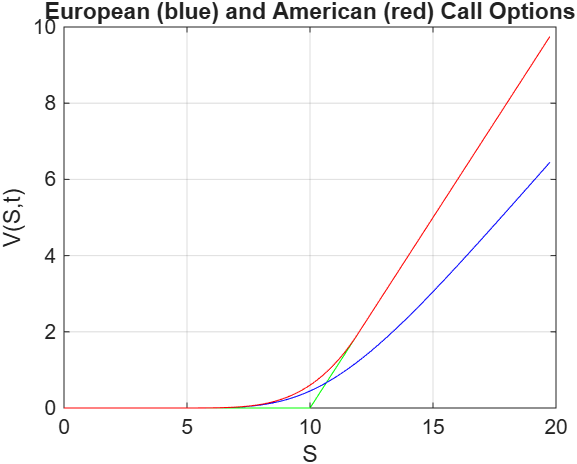
\includegraphics[width=0.8\textwidth]{media2/media/image71.png}
    \caption{Comparison of European (blue) and American (red) Call option prices today against the payoff at maturity (green) with strike price $E=10$. The American option price is higher than the European counterpart due to the added flexibility of early exercise.}
    \label{fig:your_label_name}
\end{figure}


% ==========================================
\chapter{Conclusion}
\label{ch:conclusion}
This research has presented a detailed investigation of the mathematical modeling, physical derivation and numerical approximation of partial differential equations, with applications in both engineering and quantitative finance. The study attempts to establish a connection between physical conservation laws, stochastic processes and finite difference methods, so that theoretical concepts can be linked with practical computational applications. Throughout this work, it was observed that analytical methods are very useful, however they also possess certain limitations, specially when dealing with complicated real-world problems. Therefore, numerical techniques become an essential tool for obtaining approximate but reliable solutions.

In the first part of this study, several governing equations were derived from basic physical principles and stochastic modeling approaches. The 1-dimensional transient heat equation was derived using Fourier's law of heat conduction together with the conservation of energy principle for a homogeneous and isotropic medium. Afterwards, this formulation was extended to two-dimensional systems to obtain a more general diffusion model. In a similar way, the wave equation was derived using Newtonian mechanics in order to describe the spatial and temporal behavior of transverse vibrations in an elastic string under tension.

Aside from traditional engineering applications, this study also explored financial mathematics through the derivation of the Black-Scholes partial differential equation. The derivation depends on stochastic calculus, Ito's lemma and the no-arbitrage principle. Black-Scholes model shows how PDE theory is not limited to physics only, but also it can be applied in finance by transforming the random movement of asset prices into a deterministic boundary value problem. This connection between mathematics, physics and finance is quite interesting and demonstrates the broad applicability of partial differential equations.

Since exact analytical solutions aren't always available and are often restricted by boundary conditions or domain geometry, the second part of this research focused on finite difference methods (FDMs). Different numerical schemes were examined for hyperbolic equations, particularly the advection and wave equations. The results showed that there’s an important trade-off between stability, accuracy and numerical dissipation.

The Forward in Time Central in Space scheme was found to be unconditionally unstable for the pure advection equation, making it unsuitable for long-time simulations. Although the method is easy to implement, its numerical solution becomes unstable very quickly. On the other hand, the Lax--Friedrichs method improved the stability of the solution, but introduced numerical diffusion which gradually reduced the wave amplitude and smoothed the wave profile. The Staggered Leapfrog method, however, provided much better results. It remained stable under the CFL condition and preserved the wave shape more effectively, while maintaining higher accuracy and lower numerical diffusion.

The Crank--Nicolson implicit approach and the FTCS explicit scheme were compared for parabolic diffusion problems. Since solving a set of equations is not necessary, the explicit technique is computationally easy. Nevertheless, it is conditionally stable and has to meet the Von Neumann stability criterion, $r = \alpha \Delta t / (\Delta x)^2 \le 0.5$.
This restriction often requires very small time steps, which increases the total computational time. In contrast, the Crank--Nicolson method is unconditionally stable and second-order accurate in both space and time. Although each time step requires solving a tridiagonal system of equations, the method allows larger time steps and therefore becomes more efficient for long-time diffusion simulations, even though the implementation is slightly more complicated.

The finite difference techniques developed in this research were also applied to solve the Black--Scholes PDE for pricing financial derivatives. Explicit and fully implicit schemes were implemented in MATLAB for pricing European call options. The explicit scheme produced accurate option prices when the mesh size and time step were chosen carefully, while the fully implicit method provided unconditional stability, although with a slight numerical damping effect. Among these methods, the Crank--Nicolson scheme gave the most balanced performance by providing second-order temporal accuracy and improved resolution near the strike price, where the payoff function is not smooth.

Furthermore, the research also considered American options, which can be exercised before maturity. This early exercise feature introduces a free-boundary problem where the option value must satisfy the inequality $V(S,t) \ge \max(S-E, 0)$.
By incorporating this constraint into the explicit finite difference formulation, the early exercise boundary was tracked at every time step. This result shows that numerical methods can be adapted to solve more complicated financial problems as well, although the implementation becomes somewhat challenging.

In conclusion, this thesis demonstrates that different numerical schemes may converge to similar solutions when very fine grids are used, but their stability, diffusion and dispersion properties differ significantly. Therefore, selecting an appropriate numerical method depends not only on accuracy requirements but also on computational cost and the nature of the problem itself. In some cases a simpler method may be sufficient, while for more demanding applications a more stable and accurate scheme becomes necessary.

\section{Future Directions}

While this research has provided a strong theoretical and computational basis for solving partial differential equations in engineering and finance, there are still many directions in which this work can be extended further.

\subsection{Advanced Financial Modeling and Stochastic Volatility}

The Black--Scholes model is most important model in financial mathematics, but it assumes constant volatility and log-normal asset returns. In reality, market volatility changes with time and market conditions. Thus, future work may investigate stochastic volatility models, especially Heston model, in which volatility itself behaves as a stochastic process. In addition, jump-diffusion models such as the Merton model can also be explored to describe sudden market changes and discontinuous price movements.

Moreover, the numerical techniques established in this study may be extended to more complicated derivatives, such as Asian, Barrier and Basket options. Solving these higher-dimensional and path-dependent problems is more difficult, and may require advanced methods such as Alternating Direction Implicit (ADI) schemes or operator splitting approaches to reduce computational complexity.

\subsection{Advanced Discretization Frameworks and Complex Geometries}

The finite difference methods used in this study are quite efficient for regular and structured grids. However, their application becomes difficult when the geometry of the domain is irregular or complicated. Therefore, future investigations may focus on the Finite Element Method (FEM) and the Finite Volume Method (FVM), which are more suitable for handling complex geometries and non-uniform meshes.

In addition, Spectral Methods may also be considered for problems requiring very high accuracy and fast convergence. These methods are especially useful for smooth problems involving wave propagation, although their implementation can sometimes become mathematically involved.

\subsection{Non-linear PDEs and Multi-Physics Systems}

The present study mainly focused on linear second-order partial differential equations. Future research may extend these ideas to non-linear equations such as Burgers' equation, the Korteweg--de Vries (KdV) equation and the Navier--Stokes equations. These equations have important applications in fluid dynamics, shock waves and soliton theory.

Furthermore, multi-physics systems may also be investigated by coupling different physical models together. For example, heat and wave equations can be solved simultaneously to study thermo-mechanical effects in materials subjected to vibrations and thermal loading. Such models are more realistic, though they are also more computationally demanding.

\subsection{High-Performance Computing and Machine Learning}

As numerical models become larger and more complex, the computational cost increases rapidly. Future work may therefore focus on parallel computing techniques and GPU acceleration using frameworks such as CUDA or OpenCL. These technologies can considerably reduce the computation time for large-scale simulations.

Another promising direction is the use of Physics-Informed Neural Networks (PINNs). Unlike traditional mesh-based methods, PINNs incorporate the governing differential equations directly into the neural network training process and provide a continuous approximation of the solution. Comparing the accuracy and computational efficiency of PINNs with classical finite difference and Crank--Nicolson methods would be an interesting extension of this research, and may provide new possibilities for solving complex mathematical models in future studies.

% ==========================================
% BIBLIOGRAPHY
% ==========================================
\addcontentsline{toc}{chapter}{References}
\bibliographystyle{unsrt} % Changed from 'plain' to 'unsrt'
\bibliography{references}
%%ho gya hay sahiii, bas aik word change karna tha
\end{document}